% Copyright (c) 2026 by C. Klukas.
% Licensed under the MIT License. See LICENSE for details.
%
% Paglets, the C++ edition: the paper. Chapters are in chapters/; code
% excerpts and result tables between `% snippet:` and `% results:` markers
% are generated by paglets-docs-sync from the sources (see the Makefile).

% Copyright (c) 2026 by C. Klukas.
% Licensed under the MIT License. See LICENSE for details.
%
% The preamble of paglets-cpp.tex, shared with tools/check-chapter.sh.

\documentclass[11pt,a4paper]{article}

\usepackage[T1]{fontenc}
\usepackage[utf8]{inputenc}
\usepackage{libertinus}
\usepackage{microtype}
\usepackage[a4paper,margin=26mm,headheight=22pt]{geometry}
\usepackage{amsmath}
\usepackage{amssymb}
\usepackage{booktabs}
\usepackage{caption}
\usepackage{enumitem}
\usepackage{fancyhdr}
\usepackage{float}
\usepackage{graphicx}
\usepackage{needspace}
\usepackage{xcolor}
\usepackage{tikz}
\usepackage{listings}
\usepackage{titlesec}
\usepackage{appendix}
\usepackage{hyperref}
\usepackage{url}
\usetikzlibrary{arrows.meta,fit,positioning,shapes.misc,calc,decorations.pathreplacing}

\definecolor{pagletsBlue}{HTML}{1F5A85}
\definecolor{pagletsInk}{HTML}{1F2933}
\definecolor{pagletsMuted}{HTML}{5F6B76}
\definecolor{pagletsRule}{HTML}{B8C7D3}
\definecolor{pagletsCode}{HTML}{F6F8FA}
\definecolor{pagletsGreen}{HTML}{1B7F4B}
\definecolor{pagletsAmber}{HTML}{A86400}
\definecolor{pagletsRed}{HTML}{C0352B}

\hypersetup{
  colorlinks=true,
  linkcolor=pagletsBlue,
  citecolor=pagletsBlue,
  urlcolor=pagletsBlue,
  pdftitle={Paglets: Mobile Agents as Migrating WebAssembly Instances},
  pdfauthor={Christian Klukas}
}

\AtBeginDocument{\color{pagletsInk}}

\titleformat{\section}
  {\Large\bfseries\color{pagletsBlue}}
  {\thesection}{0.75em}{}
\titleformat{\subsection}
  {\large\bfseries\color{pagletsBlue!85!black}}
  {\thesubsection}{0.65em}{}
\titleformat{\subsubsection}
  {\normalsize\bfseries\color{pagletsBlue!75!black}}
  {\thesubsubsection}{0.6em}{}
\titlespacing*{\section}{0pt}{2.6ex plus 0.6ex minus 0.2ex}{1.2ex}
\titlespacing*{\subsection}{0pt}{2.0ex plus 0.4ex minus 0.2ex}{0.8ex}
\titlespacing*{\subsubsection}{0pt}{1.6ex plus 0.3ex minus 0.2ex}{0.6ex}

\captionsetup{
  font=small,
  labelfont={bf,color=pagletsBlue},
  labelsep=period
}

\setlist{itemsep=0.25em,topsep=0.45em}
\renewcommand{\arraystretch}{1.05}

\pagestyle{fancy}
\fancyhf{}
\fancyhead[L]{\small\textsc{Paglets: the C++ edition}}
\fancyhead[R]{\small\thepage}
\renewcommand{\headrulewidth}{0.25pt}
\renewcommand{\headrule}{\hbox to\headwidth{\color{pagletsRule}\leaders\hrule height \headrulewidth\hfill}}
\renewcommand{\footrulewidth}{0pt}

\renewenvironment{abstract}
  {\begin{center}\begin{minipage}{0.92\linewidth}\small\noindent\textbf{Abstract.}\quad}
  {\end{minipage}\end{center}\vspace{0.6em}}

% -- code -----------------------------------------------------------------
% paglets-docs-sync renders snippets as lstlisting blocks of these styles,
% and puts the source path into a caption with \src.
\newcommand{\src}[1]{{\normalfont\footnotesize\color{pagletsMuted}(\texttt{#1})}}
\newcommand{\code}[1]{\texttt{#1}}

\lstdefinestyle{paglets-base}{
  basicstyle=\footnotesize\ttfamily,
  keywordstyle=\color{pagletsBlue},
  commentstyle=\color{pagletsMuted}\itshape,
  stringstyle=\color{green!35!black},
  showstringspaces=false,
  breaklines=true,
  breakatwhitespace=true,
  backgroundcolor=\color{pagletsCode},
  frame=single,
  framerule=0.3pt,
  rulecolor=\color{pagletsRule},
  columns=fullflexible,
  keepspaces=true,
  tabsize=4,
  captionpos=b,
  aboveskip=0.8em,
  belowskip=0.6em,
  xleftmargin=0.2em,
  xrightmargin=0.2em
}
\lstdefinestyle{paglets-cpp}{
  style=paglets-base,
  language=C++,
  morekeywords={override,final,constexpr,consteval,nullptr,noexcept,co_await,co_return,requires,concept,
                int8_t,int16_t,int32_t,int64_t,uint8_t,uint16_t,uint32_t,uint64_t,size_t,
                string,string_view,vector,optional,expected,unique_ptr,shared_ptr,function}
}
\lstdefinestyle{paglets-cmake}{style=paglets-base,language=[Visual]Basic,keywords={}}
\lstdefinestyle{paglets-bash}{style=paglets-base,language=bash}
\lstdefinestyle{paglets-json}{style=paglets-base,language={},keywords={}}
\lstdefinestyle{paglets-yaml}{style=paglets-base,language={},keywords={}}
\lstdefinestyle{paglets-text}{style=paglets-base,language={},keywords={}}
\lstset{style=paglets-cpp}
\renewcommand{\lstlistingname}{Listing}

% -- figures --------------------------------------------------------------
\tikzset{
  box/.style={draw=pagletsRule,fill=pagletsCode,rounded corners=2pt,line width=0.45pt,align=center,
              inner xsep=7pt,inner ysep=6pt,font=\small},
  plain/.style={draw=pagletsRule,fill=white,rounded corners=2pt,line width=0.45pt,align=center,
                inner xsep=6pt,inner ysep=5pt,font=\small},
  state/.style={draw=pagletsBlue,fill=white,rounded corners=4pt,line width=0.6pt,align=center,
                inner xsep=8pt,inner ysep=6pt,font=\small},
  event/.style={font=\footnotesize\color{pagletsMuted},align=center},
  arrow/.style={-{Latex[length=2.1mm,width=1.6mm]},draw=pagletsBlue,line width=0.55pt},
  both/.style={{Latex[length=2.1mm,width=1.6mm]}-{Latex[length=2.1mm,width=1.6mm]},draw=pagletsBlue,line width=0.55pt},
  dashedarrow/.style={-{Latex[length=2.1mm,width=1.6mm]},draw=pagletsMuted,line width=0.5pt,dashed},
  lifeline/.style={draw=pagletsRule,line width=0.5pt,dashed},
  msg/.style={-{Latex[length=1.9mm,width=1.4mm]},draw=pagletsBlue,line width=0.5pt,font=\footnotesize}
}

\newcommand{\paglets}{Paglets}
\newcommand{\paglet}{paglet}



\title{\color{pagletsBlue}\Large\bfseries Paglets: Mobile Agents as Migrating WebAssembly Instances\\[0.35em]
  \normalsize\normalfont\color{pagletsMuted}State capture between handler calls, migration and replicated execution}
\author{\normalsize Christian Klukas}
\date{\normalsize October 2026 \quad\textcolor{pagletsMuted}{(paglets/cpp 0.2.0)}}

\begin{document}

\maketitle
\thispagestyle{fancy}

% Copyright (c) 2026 by C. Klukas.
% Licensed under the MIT License. See LICENSE for details.

\begin{abstract}
To be written.
\end{abstract}


\section{Introduction}\label{sec:introduction}
% Copyright (c) 2026 by C. Klukas.
% Licensed under the MIT License. See LICENSE for details.

\subsection{Mobile agents, again}\label{sec:introduction-agents}

A mobile agent is a program that moves itself, with its state, to the
machine where the data or the resource is, works there, and moves on.
The case for it was made in the 1990s: fewer round trips over slow
links, work that continues while the client is disconnected, services
that are extended by code that arrives rather than by code that is
installed \cite{lange1999seven,harrison1995mobileAgents}. Aglets, the
system that fixed the vocabulary, made agents Java objects with a
lifecycle of creation, cloning, dispatch, deactivation and disposal,
each with a callback, reached through proxies that forward messages to
the agent wherever it is \cite{lange1997aglets,lange1998aglets}.

The first generation had three problems that were design problems, not
accidents. An agent moved as a serialized Java object, so what travelled
was decided by what the author marked serializable, and the classes had
to be present on the destination or fetched from a code base. The Java
virtual machine does not expose the state of a thread, so execution could
not move: the agent's \code{run()} started again from its beginning on
the new host, the weak mobility of Fuggetta et al.\
\cite{fuggetta1998mobility}. And a host ran foreign bytecode inside its
own virtual machine, protected by the Java security model alone, which
was the doubt raised by Harrison, Chess and Kershenbaum before the
systems existed \cite{harrison1995mobileAgents}; the design space of
code shipping, state capture and security is surveyed by Karnik and
Tripathi \cite{karnik1998design}. Serialization that captures too much
or too little, no execution state and no sandbox that one could trust
with a stranger's code: these were the reasons to prefer remote calls,
and remote calls won.

\subsection{What WebAssembly changes}\label{sec:introduction-wasm}

WebAssembly \cite{haas2017wasm} changes the trade-offs of each of the
three. It is a portable binary instruction set with a formal semantics,
compiled from C and C++ by clang and from other languages by their own
toolchains. An instance of a module has one linear memory, a contiguous
array of bytes that only the instance's own code and its host can read
or write, and a set of globals; a C++ program compiled for it keeps its
heap and its shadow stack in that memory. Between two calls into the
instance, the memory and the mutable globals are its complete state, and
the specification defines both without reference to the host, the CPU
or the operating system. The instance is sandboxed by construction: it
reaches the outside only through the functions its host provides as
imports, and a module that imports anything else cannot be
instantiated. Small
runtimes embed in a C program; \paglets{} uses WAMR \cite{wamr}. What
WebAssembly does not give is execution state across a call: a running
function's stack is the runtime's, not the module's. The design of
\paglets{} accepts this and moves agents only between calls.

\subsection{The idea}\label{sec:introduction-idea}

A \paglet{} is a WebAssembly module, named by the SHA-256 hash of its
bytes, together with one instance of it. Its whole state is the
instance's linear memory and exported mutable globals; a \emph{memory
image} of these, the non-zero 64\,KB pages with their hashes and the
globals, is all a host needs to store it, copy it or send it to another
host. A \paglet{} is \emph{created} from a module, with start arguments
and the capabilities its creator passes. It \emph{handles} messages,
requests and timers, one call at a time, through handlers that must
return within a time budget. It is \emph{dispatched} to another host by
a transfer ticket that names a host, a label, a service offer or
\code{any}; the destination fetches the module by hash if it lacks it
and receives the pages it does not hold, and the \paglet{} continues
there with its next message. It is \emph{cloned}, on its host or onto
another one, with a copy of its memory. It is \emph{deactivated} to an
image and \emph{activated} by the next message, timer or wake-up, and
on a host with a state directory it resumes from its last image after
the host restarts. It is
\emph{disposed}, or it ends by a trap. Every transition is a hook the
\paglet{} may implement, and every failure of a transition is a report
it receives as a message. The host that runs it, \code{paglets-host},
keeps the instance in a worker process that the operating system
confines, and belongs to a \emph{mesh}: hosts that share a signed
ledger of members, trusted modules and policy, and nothing else.

\subsection{Design principles}\label{sec:introduction-principles}

Five principles shape the system.

\begin{itemize}
\item \emph{State is the memory image.} No \paglet{} serializes
  anything: a \code{std::vector} in a member moves as the bytes it
  occupies, and nothing in memory can be left behind, because there is
  no list of what to take. The price is a fixed memory limit
  (16\,MB) and images that keep every page that was ever non-zero
  (Sections~\ref{sec:movement} and \ref{sec:discussion}).
\item \emph{Events between handlers.} The host calls into an instance
  from one thread at a time and takes images only between calls. A move,
  a clone or a deactivation requested inside a handler takes effect
  after the handler returns, in a fixed order, and a hook is a call like
  any other. Failures arrive as reports (\code{on\_move\_failed},
  \code{on\_undelivered}, \code{on\_recovered}), not as exceptions
  (Section~\ref{sec:lifecycle}).
\item \emph{Capabilities, not addresses.} A \paglet{} has no address.
  It reaches another \paglet{}, a service or a resource only through a
  capability in a table the host keeps for it: an endpoint, a reply
  capability, a timer, a directory or an artifact. Capabilities move
  with the \paglet{} under a rule per kind, and location records let an
  endpoint find its target after a move (Sections~\ref{sec:model} and
  \ref{sec:communication}).
\item \emph{A signed mesh.} Admins, hosts, owners and signers hold
  Ed25519 keys. Membership, module trust, policy and grants are signed
  records in a grow-only ledger spread by gossip; hosts talk inside
  mutually authenticated, end-to-end encrypted channels; and a
  \paglet{} reaches host resources only through system \paglet{}s, within
  the policy (Section~\ref{sec:mesh}).
\item \emph{Verification in the same code base.} The fault-tolerance
  protocol of zombie \paglet{}s is a pure C++ transition function. The
  guest SDK runs it, an explicit-state model checker in the repository
  explores it, a simulator runs it under time and random faults, and
  live traces are checked against its transition table
  (Section~\ref{sec:zombies}).
\end{itemize}

\subsection{Contributions}\label{sec:introduction-contributions}

\begin{enumerate}
\item A programming model and an ABI (v1, minor version 1.2,
  Appendix~\ref{app:abi}) for mobile agents as WebAssembly instances:
  fourteen imports, six required exports, seven event kinds and three
  reports, covered by 41 conformance tests.
\item A host runtime with sandboxed worker processes on Linux and macOS
  (Windows experimental), whose memory images are independent of the
  CPU and the operating system: one build of the counter module (an
  ABI~v0 build of the feasibility milestone) was moved in four transfers between macOS arm64, Linux arm64 and an x86-64
  build under Rosetta~2 (Section~\ref{sec:evaluation}).
\item A move protocol between hosts that sends only the pages the
  destination lacks (2.2 pages on average on repeated moves of a 4\,MB
  \paglet{}, after 66 on the first), with location records on three
  hosts chosen by consistent hashing, so that endpoints keep working
  across moves (Sections~\ref{sec:movement} and \ref{sec:communication}).
\item A mesh bound only by a signed ledger: four key roles, quorums,
  gossip, Noise channels inside HTTPS, allow/ask/deny policy with
  grants, system \paglet{}s as the only path to resources
  (Section~\ref{sec:mesh}), and relays for hosts without an inbound port
  (Section~\ref{sec:communication-relays}).
\item Zombie \paglet{}s, whose protocol is checked in the repository:
  four invariants and two recoverability goals hold in ten two-replica
  worlds explored completely (up to 22.4 million states), the invariants
  hold to depth 11 in two three-replica worlds, 10\,000 timed runs with
  119\,289 faults show no failure, and a live run with a failure
  schedule on three machines conforms to the specification
  (Section~\ref{sec:zombies}).
\item Tools that stay true to the sources: interface descriptions inside
  the module, a command line and a web UI built from them, and a
  generator that renders the code excerpts and result tables of the
  documentation and of this paper from the sources, checked by a test
  (Section~\ref{sec:tools}).
\item An evaluation on three real machines and in a test suite of 252
  cases run in two modes: request round trips of 1.16--5.16\,ms mean,
  file transfers of 20--40\,MB/s, 100\,000 hexadecimal digits of $\pi$
  in 313\,s on three hosts, and what is not measured
  (Section~\ref{sec:evaluation}).
\end{enumerate}

\subsection{The paper}\label{sec:introduction-outline}

Section~\ref{sec:background} places \paglets{} among Aglets, weak and
strong mobility, process migration, actors and earlier Wasm snapshots,
and names the Python edition of \paglets{}, whose application note
\cite{klukas2026pagletsNote} describes a system that moves a declared
state record between hosts sharing the code; the C++ edition
\cite{pagletsCpp,pagletsCppDocs} keeps its concepts and none of its
formats. Section~\ref{sec:model} defines the model: module and instance,
identity, messages, typed payloads, capabilities and the import set.
Section~\ref{sec:lifecycle} gives the states, the hooks and the order in
which the host runs them. Section~\ref{sec:movement} describes the
memory image, what does not move, transfer tickets and the two-host
protocol. Section~\ref{sec:communication} shows how an endpoint reaches
a \paglet{} that has moved. Section~\ref{sec:mesh} describes the ledger,
passports, policy and system \paglet{}s. Section~\ref{sec:zombies}
presents zombie \paglet{}s and what was verified about them.
Section~\ref{sec:tools} covers interface descriptions, the command line,
the web UI and the documentation generator. Section~\ref{sec:evaluation}
reports the measurements, Section~\ref{sec:discussion} the costs and
limits, and Section~\ref{sec:conclusion} concludes. The appendices list
the ABI (\ref{app:abi}), the complete example \paglet{}s
(\ref{app:examples}), the hooks and ordering guarantees
(\ref{app:events}) and how to reproduce the results
(\ref{app:reproduce}).

\section{Background and Related Work}\label{sec:background}
% Copyright (c) 2026 by C. Klukas.
% Licensed under the MIT License. See LICENSE for details.

\paglets{} revisits a programming model from the 1990s with a runtime that
did not exist then. This chapter places it: the Aglets lifecycle it keeps,
the kinds of mobility that mobile-agent systems and process migration
offer, the actor systems that solved placement differently, and
WebAssembly as the unit that moves. It ends with the Python edition of
\paglets{} and what the C++ edition changes.

\subsection{Aglets and the agent lifecycle}\label{sec:background-aglets}

Aglets, developed at IBM's Tokyo Research Laboratory, made mobile agents
Java objects \cite{lange1997aglets,lange1998aglets}. An aglet lives in an
\emph{aglet context}, the execution environment a server such as Tahiti
offers \cite{ferrari2004manual}. Other code never holds the aglet itself;
it holds an \emph{aglet proxy}, which shields the aglet and forwards
messages to it wherever it is. The programming model is a small set of
lifecycle operations with a callback for each \cite{langeOshimaAgletApi}:

\begin{itemize}
\item \emph{creation} and \emph{cloning} (\code{onCreation},
  \code{onClone});
\item \emph{dispatch} to another context and \emph{retraction} back
  from it (\code{onDispatching}, \code{onArrival} and
  \code{onReverting});
\item \emph{deactivation} to secondary storage and \emph{activation}
  from it (\code{onDeactivating}, \code{onActivation});
\item \emph{disposal} (\code{onDisposing});
\item \emph{messages}, handled by \code{handleMessage}, sent through the
  proxy synchronously, as a future or one-way.
\end{itemize}

After creation, cloning, activation or arrival the runtime calls
\code{run()}, the aglet's own thread of control. An aglet moves as a
Java-serialized object over the Agent Transfer Protocol; the thread does
not move, so \code{run()} starts again from its beginning on the new
host. IBM's own researchers had asked in 1995 whether mobile agents are a
good idea at all \cite{harrison1995mobileAgents}; Lange and Oshima later
answered with seven reasons to move computation rather than data
\cite{lange1999seven}. The design space of such systems, from code
shipping to security, is surveyed by Karnik and Tripathi
\cite{karnik1998design}. Aglets was later released as an open-source
project on SourceForge \cite{agletsSourceForge}.

\paglets{} keeps this vocabulary. A \paglet{} is created or cloned,
dispatched, deactivated and activated, disposed; it arrives; it handles
messages; and every Aglets callback except \code{onReverting} has a
counterpart among its hooks: \code{on\_created}, \code{on\_cloned},
\code{on\_dispatching}, \code{on\_arrived}, \code{on\_deactivating},
\code{on\_activated} and \code{on\_disposing}
(Section~\ref{sec:lifecycle}). \paglets{} adds \code{on\_move\_failed},
\code{on\_undelivered} and \code{on\_recovered}, reports for which Aglets
has no callback. Two things differ at this level. There is no
\code{run()}: a \paglet{} has no thread of its own, and all its code runs
in handlers that the host calls one at a time. And there is no retraction
as a named operation: a \paglet{} that should come back is dispatched
again, by itself or by its owner from the command line
(Section~\ref{sec:tools}). The proxy survives as the \emph{endpoint}, a
capability that reaches a \paglet{} wherever it is
(Section~\ref{sec:communication}).

\subsection{Weak and strong mobility}\label{sec:background-mobility}

Fuggetta, Picco and Vigna separate the state of a running program into
its code, its data (the heap and the variables) and its execution state
(the stack and the program counter), and classify mobility by what moves
\cite{fuggetta1998mobility}. \emph{Strong} mobility moves all three: the
program continues on the new host with the statement after the jump.
Agent Tcl does this by capturing the interpreter's state \cite{gray1996agentTcl}.
\emph{Weak} mobility moves code and data only; execution restarts at an
entry point. Java systems on the standard virtual machine are weak,
because the virtual machine does not expose the state of a thread;
Aglets' restart of \code{run()} is the visible consequence.
Table~\ref{tab:mobility-kinds} puts these kinds next to process migration
and the two \paglets{} editions.

\begin{table}[htbp]
\centering\small
\caption{Kinds of mobility by what moves and where execution resumes.}
\label{tab:mobility-kinds}
\begin{tabular}{p{0.19\linewidth}p{0.35\linewidth}p{0.19\linewidth}p{0.15\linewidth}}
\toprule
Kind & What moves & Resumes at & Examples \\
\midrule
Process migration & the address space, registers, kernel state (files, sockets) & the interrupted instruction & CRIU \cite{criu}, the systems in \cite{milojicic2000migration} \\
Strong mobile agents & code, data, interpreter stack and program counter & the statement after the jump & Agent Tcl \cite{gray1996agentTcl} \\
Weak mobile agents & code (or a reference to it) and serialized object fields & \code{run()} & Aglets \cite{lange1998aglets} \\
Explicit state & a declared state record; code installed on every host & a lifecycle hook & \paglets{}, Python edition \cite{klukas2026pagletsNote} \\
Memory image & the module (by hash) and the linear memory with its globals, as bytes & \code{on\_arrived}, then the next handler & \paglets{}/cpp (this paper) \\
\bottomrule
\end{tabular}
\end{table}

In these terms \paglets{}/cpp is weak mobility: a \paglet{} moves only
between two handler calls, when no code of the \paglet{} is running, and
it resumes with the next event or message. What distinguishes it is the
data that moves. It is not a record the author declared, but the whole
linear memory of the WebAssembly instance together with its exported
mutable globals, taken as bytes. The heap, every C++ object, and the
C/C++ shadow stack that the compiler keeps in linear memory are in it.
Nothing in memory is serialized, and nothing in memory can be left
behind, because there is no list of what to take; what lives outside
memory is the subject of Section~\ref{sec:movement}. The Wasm operand
stack and the native call stack hold values only during a call, and at
the moment of the move there is no call. Moving inside a handler would
need the stack as well; the Asyncify transformation
\cite{zakai2019asyncify} and the proposed stack-switching instructions
could provide it, and mid-handler moves are a research item, not a
feature (Section~\ref{sec:discussion}).

\subsection{Process migration and actors}\label{sec:background-actors}

Process migration moves a whole operating-system process: its address
space, registers and, as far as possible, its kernel state
\cite{milojicic2000migration}. CRIU does this on Linux today, as
checkpoint and restore of process trees from user space \cite{criu}. The
unit is transparent to the program, which is its strength, and bound to
one kernel, one architecture and the same installed libraries, which is
its limit. A \paglet{} is a smaller unit with an explicit boundary: the
paglet ABI (Appendix~\ref{app:abi}). What a \paglet{} holds outside its
memory, such as an endpoint to another \paglet{} or a grant for a host
resource, is a capability with a defined mobility rule; the host
re-creates it on the destination or reports it lost
(Section~\ref{sec:movement}). The image is independent of the CPU and
the operating system; the project's feasibility milestone moved images
between macOS and Linux hosts, and between arm64 hosts and an x86-64
build of the host run under Rosetta~2, without translation
(\cite{pagletsCpp}; the milestone record in the repository's planning
documents, and Section~\ref{sec:evaluation}).

The actor model gives the other half of the lineage. An actor handles one
message at a time, creates actors and sends messages to the actors it
knows \cite{hewitt1973actor}. Erlang made this an engineering practice:
isolated processes with their own heaps, message passing as the only
interaction, supervision trees, and the rule that a failed process is
restarted rather than repaired \cite{armstrong2003thesis}. Orleans'
\emph{virtual actors} (grains) remove placement from the programmer: a
grain always exists, the runtime activates it on some server when a
message arrives and deactivates it when idle; its state can be persisted
and reloaded, and in the design as published a grain is never moved as a
running object \cite{bernstein2014orleans}. Later releases added the
migration of an idle activation to another server, its in-memory state
dehydrated on one side and rehydrated on the other
\cite{orleansGrainMigration}.

A \paglet{} is an actor in the first sense: one handler at a time, and
other \paglets{} reachable only through endpoints it was given. It
differs from grains in that placement is a decision of the \paglet{} or
its owner, who name the destination in a transfer ticket (a host, a
label, a service offer or \code{any}; for the last three the host picks a
matching host), not of a scheduler that moves \paglets{} on its own, and
the state moves as a running instance's memory rather than through a
store. An inactive \paglet{} resembles a deactivated grain: an image on
disk, restored when a message or a timer arrives. Fault tolerance
follows Erlang rather than Orleans: a zombie \paglet{}
(Section~\ref{sec:zombies}) has a replica on every host of the mesh that
offers the \code{zombies} service, and the replicas run a protocol to
take over, instead of relying on a shared store. The host restarts no
\paglet{} that trapped: as in Erlang, a crash ends the process, and
recovery is the job of another one.

\subsection{WebAssembly as the unit that moves}\label{sec:background-wasm}

WebAssembly is a portable binary instruction format with a formal
semantics, designed so that a module validates and compiles fast and runs
inside a sandbox \cite{haas2017wasm}. A paglet module declares functions,
globals, tables and exactly one linear memory (the paglet ABI requires
it, exported as \code{memory}), a contiguous array of bytes that the
module addresses with 32-bit offsets; an instance is the module together
with that memory, its globals and its tables. A C++ program compiled with
the WASI toolchain keeps its heap and its shadow stack in linear memory;
the only other state that outlives a call is the stack pointer, a mutable
Wasm global (the single mutable global of a C/C++ guest). This is the
fact on which \paglets{}/cpp rests: between two calls into the instance,
the linear memory and the mutable globals are the complete state, and the
specification defines both without reference to the host.

Runtimes differ in how they execute a module. Wasmtime, the Bytecode
Alliance's runtime, compiles modules with Cranelift and implements the
WASI system interface \cite{wasmtime,wasi}. WAMR (WebAssembly Micro
Runtime) is a small C runtime for embedding, with a classic and a fast
interpreter and optional ahead-of-time and just-in-time modes
\cite{wamr}. \paglets{}/cpp embeds WAMR in its worker processes and runs
the fast interpreter by default (the classic interpreter is a build
option); neither the ahead-of-time nor the just-in-time modes are built
(\code{cpp/cmake/PagletsWamr.cmake}). The interpreter costs speed
(Section~\ref{sec:evaluation}). It is the portable default: WAMR's
ahead-of-time mode needs an LLVM-based compiler (\code{wamrc}) and has
not been measured, and the design keeps compiled forms, where they exist,
in a per-host cache that is never sent between hosts \cite{pagletsCpp}.
The image is independent of the execution mode either way: it holds the
linear memory and the globals, and no code. Of WASI a \paglet{} may
import only a subset, listed in Appendix~\ref{app:abi}; everything else
it reaches through the \code{paglets} import module.

The idea of treating an instance's memory as a snapshot is not new. Wizer
runs a module's initialization ahead of time and writes the resulting
memory and globals into the data segments of a new module, so that the
module starts initialized \cite{wizer}. It uses the same observation for
a different purpose; the initialization it snapshots may not call
imported functions (WASI calls only when explicitly allowed), and the
module may not import globals, tables or memories. Research on
checkpointing and migrating running Wasm programs attacks the harder
case: Tamura et al. instrument ahead-of-time compiled code and record
stack maps, so that at designated program points the machine state can
be turned back into Wasm state (operand stack and locals) and restored on
another instruction set \cite{tamura2025crossisa}. \paglets{} needs none
of this because it moves at quiescent points only; it trades the ability
to move mid-computation for an image that is a plain copy of memory. Long
computations are therefore written in steps, as the examples in
Sections~\ref{sec:zombies} and \ref{sec:evaluation} show; the host
enforces this with a time budget per handler call (5~s by default), after
which the \paglet{} fails.

\subsection{The Python edition and what the C++ edition changes}\label{sec:background-python}

The first edition of \paglets{} is a Python package
\cite{pagletsSoftware,klukas2026pagletsNote}. Its mobile state is a
dataclass the author declares, and a move carries that state with the
names of the paglet and state classes, which every host must be able to
import; code is never uploaded. Each active paglet runs in a child
process of the host, and the hosts of a mesh trust each other and may
share an API key.

The C++ edition keeps the concepts (hosts, paglets, messages, a mesh,
services, compute slots) and none of the formats; the two editions do not
exchange paglets \cite{pagletsCppDocs}. It changes five things.

\begin{enumerate}
\item \emph{Modules are the unit of code.} A \paglet{}'s code is a
  WebAssembly module, named by its SHA-256 hash. A host that lacks a
  module fetches it from the source host or any peer and verifies the
  hash; hosts do not need the same code installed
  (Section~\ref{sec:movement}).
\item \emph{State is the memory image.} There is no state class. The
  author's objects live in linear memory, and a move sends the pages
  that changed since the destination last saw them, compressed.
\item \emph{Paglets run sandboxed.} Instances live in worker processes
  that the operating system confines (seccomp on Linux, a sandbox
  profile on macOS, a job object with a restricted token on Windows).
  A \paglet{} cannot open a file or a socket; it reaches host resources
  through system paglets, within the mesh policy
  (Section~\ref{sec:mesh}).
\item \emph{A signed ledger replaces the API key.} Hosts, admins, owners
  and signers have Ed25519 keys. Membership, module trust, policy rules
  and grants are signed records, spread by gossip; hosts talk inside
  mutually authenticated, end-to-end encrypted channels
  (Section~\ref{sec:mesh}).
\item \emph{Fault tolerance with a checked protocol.} Zombie paglets
  replicate a job on every host of the mesh that offers the
  \code{zombies} service and hand it over when the main replica
  disappears. The protocol is a C++ state machine that the guest SDK runs
  and that an explicit-state model checker explores for small worlds
  (Section~\ref{sec:zombies}).
\end{enumerate}

Table~\ref{tab:background-editions} places the three systems next to each
other by concept; Section~\ref{sec:discussion-comparison} does it again
by what each one pays, with the limits that the evaluation shows.

\begin{table}[htbp]
\centering\small
\caption{Aglets and the two \paglets{} editions, by concept.}
\label{tab:background-editions}
\begin{tabular}{p{0.16\linewidth}p{0.23\linewidth}p{0.23\linewidth}p{0.23\linewidth}}
\toprule
 & Aglets & \paglets{}, Python & \paglets{}/cpp \\
\midrule
Mobile unit & Java object & dataclass state plus class names & Wasm instance: module hash plus memory image \\
Execution & \code{run()} thread, restarted after a move & a \code{run()} hook in the child process, plus handlers, serial per paglet & handlers, one at a time; no thread \\
Reaching others & proxies & proxies & endpoint capabilities only \\
Failure & --- & an active paglet is lost with its host; an inactive one survives as persisted dataclass state & a trap ends the paglet; after a host restart it resumes from its last image (default policy); zombie replicas \\
\bottomrule
\end{tabular}
\end{table}

\section{Execution Model}\label{sec:model}
% Copyright (c) 2026 by C. Klukas.
% Licensed under the MIT License. See LICENSE for details.

A \paglet{} is a WebAssembly module together with one instance of it.
This chapter takes that sentence apart: what names a \paglet{} and who
runs it, how it receives and sends messages, how payloads are typed, how
it reaches other \paglet{}s, and what it can and cannot do. The chapters
that follow build on these definitions: the lifecycle
(Section~\ref{sec:lifecycle}), moves (Section~\ref{sec:movement}),
communication while a \paglet{} moves (Section~\ref{sec:communication})
and the mesh (Section~\ref{sec:mesh}).

\subsection{A module and one instance}\label{sec:model-instance}

The \emph{module} is a core WebAssembly module for \code{wasm32}, compiled
by clang from C++ against the guest SDK (\code{cpp/sdk/}). It has exactly
one linear memory, exported as \code{memory}, and a small set of exports
the host calls (Section~\ref{sec:model-imports}). The host names a module
by the SHA-256 hash of its bytes, written in hex; adding the same bytes
twice is a no-op, and every \paglet{} record, every sender record and
every passport refers to its module by this hash.

The \emph{instance} is one WebAssembly instance of that module. The SDK
keeps a single static object of the \paglet{}'s class in the module's
linear memory. That object, everything it owns on the heap, the
registered handlers and the continuations of outstanding requests are all
bytes of that memory. The \paglet{}'s state is therefore its linear
memory plus the module's exported mutable globals (for C++ guests, the
stack pointer). A \emph{memory image} of these is all a host needs to
store a \paglet{}, to copy it, or to send it to another host
(Section~\ref{sec:movement}); no code in a \paglet{} serializes its
state.

Three values identify a \paglet{} to its host and to the mesh:

\begin{itemize}
\item The \emph{\paglet{} ID}: 32 lowercase hex digits, 16 random bytes
  drawn when the \paglet{} is created, or chosen in advance when a
  passport names it.
\item The \emph{owner}: a string the host assigns. On a single host it is
  \code{local}; in a mesh it is the key ID of the owner whose key signed
  the launch. Children and clones have the owner of their creator.
\item The \emph{trust class}: \code{roaming}, \code{resident} or
  \code{system} (Table~\ref{tab:model-trust}). The host assigns it; a
  \paglet{} never claims its own class, and a \paglet{} that arrives from
  another host is always roaming. Children are roaming. A clone keeps its
  creator's class, except that a clone of a system \paglet{} is roaming;
  a clone made on another host (Section~\ref{sec:movement}) is only
  allowed for a roaming \paglet{}.
\end{itemize}

\begin{table}[htbp]
\centering\small
\begin{tabular}{lp{68mm}lp{32mm}}
\toprule
Class & Origin & Moves & Import set \\
\midrule
\code{system} & \raggedright built into the host (native C++), or a module the ledger trusts for this class & never & \raggedright standard plus \code{paglets\_sys} \tabularnewline
\code{resident} & \raggedright meant for modules an admin installs on one host; the ledger can admit modules to the class, but no command or mesh operation creates a resident \paglet{} today & no & standard \tabularnewline
\code{roaming} & \raggedright created by an owner or by another \paglet{}, or arrived from another host & yes & standard \tabularnewline
\bottomrule
\end{tabular}
\caption{Trust classes. In the current release every system \paglet{} is native; the runtime's C++ API (\code{CreateOptions::trust}) accepts every class and the tests use it, but no command or mesh operation creates a resident \paglet{}. The classes exist in the runtime, the ledger's module trust and the sender records.}
\label{tab:model-trust}
\end{table}

A \paglet{} launched into a mesh carries a \emph{passport}: a document
signed by the owner's key that names the mesh, the owner, the module hash
and the \paglet{} ID, extended by a host-signed link for every child or
clone. A host verifies it against the ledger before it accepts the
\paglet{}, and it travels with the \paglet{}. A \paglet{} without one,
such as one started by \code{paglets-host run} on a single host, cannot
move. Section~\ref{sec:mesh-passports} gives the contents and the checks.

Figure~\ref{fig:model-architecture} shows where an instance runs. The host
process, \code{paglets-host}, starts one \emph{worker process} per
scheduler lane (two by default) and places each active \paglet{} on one of
them. The operating system sandboxes the workers: a seccomp filter on
Linux, a sandbox profile on macOS, a job object with a restricted token on
Windows. A worker can neither open files nor create sockets nor start
programs (on Windows the restricted token stops new processes and writes
to ordinary files, but reading files and network access are not
restricted yet); every effect of a \paglet{} passes through its host.
Calls between the two processes go over two shared-memory rings, one per
direction; a socket pair (two pipes on Windows) carries wake-ups and
terminations. The embedded WAMR engine runs the instances. For tests and debugging,
\code{--in-process} runs them inside the host process instead.

\begin{figure}[htbp]
\centering
\pgfdeclarelayer{background}
\pgfsetlayers{background,main}
\begin{tikzpicture}[node distance=3.5mm and 36mm]
  \node[plain,text width=44mm] (module) {\textbf{Paglet module} (Wasm)\\[1pt]\footnotesize linear memory: the \paglet{} object, its handlers, its continuations};
  \node[plain,text width=44mm,below=of module] (sdk) {\textbf{Guest SDK}\\[1pt]\footnotesize \code{Paglet}, \code{Router}, \code{Message}, \code{Endpoint}, MessagePack codecs};
  \node[plain,text width=44mm,below=of sdk] (wamr) {\textbf{WAMR engine}\\[1pt]\footnotesize instances, traps, time budgets, memory images};
  \begin{pgfonlayer}{background}
  \node[box,fit=(module)(sdk)(wamr),inner sep=7pt,label={[font=\small\bfseries\color{pagletsBlue}]above:Worker process (sandboxed)}] (worker) {};
  \end{pgfonlayer}

  \node[plain,text width=44mm,right=of module] (runtime) {\textbf{Runtime}\\[1pt]\footnotesize mailboxes, capability tables, timers, images, scheduler};
  \node[plain,text width=44mm,below=of runtime] (system) {\textbf{System \paglet{}s}\\[1pt]\footnotesize files, directory, grants, mesh-info, \ldots};
  \node[plain,text width=44mm,below=of system] (node) {\textbf{Mesh node}\\[1pt]\footnotesize moves, location records, ledger, channels};
  \begin{pgfonlayer}{background}
  \node[box,fit=(runtime)(system)(node),inner sep=7pt,label={[font=\small\bfseries\color{pagletsBlue}]above:Host process (\code{paglets-host})}] (host) {};
  \end{pgfonlayer}

  \draw[arrow] (host.west|-module) -- node[event,above,text width=28mm,font=\scriptsize\color{pagletsMuted}]{\code{paglets\_on\_event}\\\code{paglets\_on\_message}} (worker.east|-module);
  \draw[arrow] (worker.east|-sdk) -- node[event,above,text width=28mm,font=\scriptsize\color{pagletsMuted}]{\code{send}, \code{request}, \code{reply}, \code{lifecycle}, \ldots} (host.west|-sdk);
  \draw[both] (worker.east|-wamr) -- node[event,above,text width=28mm,font=\scriptsize\color{pagletsMuted}]{memory images} (host.west|-wamr);
  \node[event,text width=60mm] at ($(worker.south east)!0.5!(host.south west)+(0,-6mm)$) {Paglet ABI v1: MessagePack documents in linear memory, carried between the processes over shared-memory rings};
  \draw[dashedarrow] (host.east) -- ++(7mm,0) node[event,right,text width=12mm]{other hosts};
\end{tikzpicture}
\caption{A \paglet{} instance in a worker process and the host runtime. The host calls the module's handler exports; the SDK calls the fourteen imports of the \code{paglets} module, and the guest's C library the WASI subset of Table~\ref{tab:model-imports}. Nothing else crosses the boundary.}
\label{fig:model-architecture}
\end{figure}

\subsection{A first \paglet{}}\label{sec:model-hello}

Listing~\ref{lst:hello} is the smallest example of the repository. A
\paglet{} is a class derived from \code{paglets::Paglet}, registered with
\code{PAGLETS\_PAGLET} at namespace scope. Its constructor runs once,
when the host delivers the \code{created} event, and never again: after a
restore from a memory image the constructed object is already in the
memory. The constructor is where handlers are registered.

% snippet: cpp/examples/hello/hello.cpp [float,caption={The hello \paglet{}},label={lst:hello}]
\begin{lstlisting}[style=paglets-cpp,float,caption={The hello \paglet{} \src{cpp/examples/hello/hello.cpp}},label={lst:hello}]
// Smallest paglet: answers "greet" requests and counts them.

#include <paglets/paglet.hpp>

#include <string>

namespace {

class Hello : public paglets::Paglet {
public:
    Hello() {
        router().on<std::string>("greet", [this](const std::string& name, paglets::Message& m) {
            ++greetings_;
            m.reply("hello, " + name + " (greeting " + std::to_string(greetings_) + ")");
        });
    }

    void on_created(paglets::Started&) override {
        auto info = paglets::self_info();
        paglets::log("hello paglet created as " + (info ? info->id : std::string("?")));
    }

private:
    std::uint32_t greetings_ = 0;
};

}  // namespace

PAGLETS_PAGLET(Hello)
\end{lstlisting}
% /snippet

\code{router().on<std::string>("greet", ...)} registers a handler for
requests named \code{greet} whose body decodes as a MessagePack string.
The handler receives the decoded body and the \code{Message}, and answers
with \code{m.reply(...)}, which the SDK encodes as MessagePack again. The
count of greetings is an ordinary member: nothing saves it, it is part of
the memory image. \code{on\_created} is one of the lifecycle hooks of
Section~\ref{sec:lifecycle}; here it asks for the \paglet{}'s own record
with \code{self\_info()} and writes the ID to the host log, where a
\paglet{}'s \code{stdout} and \code{stderr} go as well. One CMake call
builds the module: \code{paglets\_add\_module(hello SOURCES hello/hello.cpp)}
(the repository's line adds \code{INTERFACE hello/interface.json}, the
interface description of Section~\ref{sec:tools}).
\code{paglets-host run hello.wasm} with \code{--call greet '"world"'}
creates a \paglet{} from it, sends the request and prints the reply as
JSON: \code{greet -> "hello, world (greeting 1)"}. Bodies on the command
line are JSON; the host converts them to MessagePack and the replies back.

\subsection{Messages, requests and timers}\label{sec:model-messages}

Every \paglet{} has a mailbox. The host delivers its messages one at a
time, by priority (0 to 7, highest first, default 3) and in arrival order
within a priority; a mailbox holds at most 1024 messages. A \paglet{}
never sees two calls at once: handlers and lifecycle hooks run one after
the other, never concurrently, and the host takes memory images only
between two calls. A \paglet{} shares memory with nothing; its only
effects are the messages it sends, the \paglet{}s it creates, the timers
it sets, its log lines and the lifecycle operations it requests. A handler
must not block, because nothing it could wait for arrives while it runs: a
reply, a service's answer or a timer is a later message. A handler that
runs longer than its time budget (5 seconds of elapsed time by default) is
terminated and the \paglet{} fails.

A delivered \code{Message} has a kind (\code{message}, \code{request},
\code{reply} or \code{timer}), a name of up to 128 bytes, a payload, a
priority, the capabilities that came with it, and for messages from other
\paglet{}s, or from the host's own tools (ID \code{host}, trust
\code{system}), a \emph{sender record} the host stamps on it: the
sender's ID, owner, trust class, module hash and host. Replies, timers and
reports from the host carry none. Three things can be sent:

\begin{itemize}
\item A \emph{message} is one-way: \code{endpoint.send(name, body)}. The
  call fails at once with \code{denied}, \code{expired} or \code{quota}
  when the endpoint does not allow the message, with \code{not\_found}
  when the target has ended, and with \code{quota} when its mailbox is
  full. With \code{SendOptions::async} the call returns as soon as the
  document is well-formed and a failure arrives later as the hook
  \code{on\_undelivered}; in a worker process this saves the round trip to
  the host.
\item A \emph{request} expects exactly one reply.
  \code{request(name, body, on\_reply)} on an endpoint returns a
  correlation ID and keeps \code{on\_reply}, the continuation. The
  receiver gets the message with a one-shot \emph{reply capability}. The
  reply arrives at priority 7 with a status: 0 and the payload for a real
  reply; otherwise \code{timeout} (30 seconds by default),
  \code{unknown\_message} (the receiver had no handler), \code{failed} (the
  receiver trapped), \code{gone} (the receiver ended or dropped the reply
  capability), or the error code the receiver's handler returned. A
  request is never asynchronous in the sense above: the call waits for the
  host to accept it.
\item A \emph{timer}: \code{after(delay\_ms, name, body)} delivers a
  message of kind \code{timer} to the \paglet{} itself after the delay.
  The returned capability cancels the timer when dropped. A \paglet{}
  holds at most 64 pending timers; they survive deactivation and wake a
  deactivated \paglet{}.
\end{itemize}

The continuation is a \code{std::function} that the SDK stores in a map
keyed by the correlation ID. The map lives in linear memory, so an
outstanding request survives deactivation and moves: the reply reaches its
continuation wherever the \paglet{} is when it arrives.
Listing~\ref{lst:pingpong-bounce} shows the shape. \code{pong\_} is the
parent's endpoint to the child, a capability
(Section~\ref{sec:model-capabilities}); \code{pending\_run\_} holds the
reply capability of the \code{run} request that started the rounds
(Listing~\ref{lst:pingpong-roles}). The parent of the ping-pong example
sends \code{ping} to its child and names the function that runs with the
reply; that function checks the status, decodes the body and sends the
next \code{ping}. No handler waits.

% snippet: cpp/examples/ping_pong/ping_pong.cpp#bounce [float,caption={A request with a continuation, and a deferred reply answered from it},label={lst:pingpong-bounce}]
\begin{lstlisting}[style=paglets-cpp,float,caption={A request with a continuation, and a deferred reply answered from it \src{cpp/examples/ping\_pong/ping\_pong.cpp}},label={lst:pingpong-bounce}]
void bounce(std::uint32_t n) {
    if (n >= target_) {
        (void)paglets::reply_to(pending_run_, n);
        (void)pong_.send("stop");
        return;
    }
    auto sent = pong_.request("ping", n, [this](paglets::Message& reply) {
        std::uint32_t value = 0;
        if (!reply.ok() || !reply.decode(value)) {
            paglets::log(paglets::abi::LogLevel::error,
                         "ping failed: " + std::string(paglets::abi::error_name(reply.status())));
            (void)pending_run_.drop();
            return;
        }
        bounce(value);
    });
    if (!sent) (void)pending_run_.drop();
}
\end{lstlisting}
% /snippet

A request is answered once. The handler answers it directly with
\code{reply} or \code{reply\_async} on the message, or it keeps the reply
capability for later: \code{defer\_reply} returns it, and
\code{reply\_to} answers with it from any later handler. This
is the \emph{deferred reply} of Listing~\ref{lst:pingpong-roles}: the
\code{run} handler cannot know its answer, which exists only after many
rounds, so it defers the reply, and \code{bounce} answers it when the
target is reached. A reply capability is an ordinary capability: it can be
transferred to another \paglet{}, which then answers in the original
receiver's place. Dropping it, as the error path of
Listing~\ref{lst:pingpong-bounce} does, answers the requester \code{gone}
at once instead of letting it wait for its timeout. A request that a
handler handled but neither answered nor deferred is answered \code{gone}
as well: the SDK drops the reply capability when the handler returns.

% snippet: cpp/examples/ping_pong/ping_pong.cpp#roles [float,caption={The ping-pong handlers: a child from the same module, a deferred reply, an asynchronous reply},label={lst:pingpong-roles}]
\begin{lstlisting}[style=paglets-cpp,float,caption={The ping-pong handlers: a child from the same module, a deferred reply, an asynchronous reply \src{cpp/examples/ping\_pong/ping\_pong.cpp}},label={lst:pingpong-roles}]
PingPong() {
    // Parent role.
    router().on<std::uint32_t>("run", [this](std::uint32_t rounds, paglets::Message& m) -> std::int32_t {
        if (pending_run_) return paglets::abi::bad_state;
        auto child = paglets::create_child(std::uint32_t{0});
        if (!child) return child.error();
        pong_ = *child;
        target_ = rounds;
        pending_run_ = m.defer_reply();
        bounce(0);
        return paglets::abi::handled;
    });
    // Child role. The reply is asynchronous: in a worker process it does
    // not wait for the host, and a failure would reach on_undelivered.
    router().on<std::uint32_t>("ping", [](std::uint32_t n, paglets::Message& m) { m.reply_async(n + 1); });
    router().on("stop", [](paglets::Message&) { (void)paglets::dispose(); });
}
\end{lstlisting}
% /snippet

\subsection{The router}\label{sec:model-router}

\code{Paglet::on\_message} receives every delivery except replies that
have a continuation and the host's reports (\code{on\_undelivered},
\code{on\_move\_failed}, \code{on\_recovered}). Its default passes the
message to the \paglet{}'s \code{Router}, a map from message names to
handlers. \code{router().on(name, f)} registers \code{f} for a name;
\code{router().otherwise(f)} catches the rest. Without either, a message
is not handled: a one-way message is dropped, a request is answered
\code{unknown\_message}. Timer messages go through
the router under the name given to \code{after}. A handler either returns
\code{void}, which counts as handled, or an \code{std::int32\_t}:
\code{abi::handled} (0), \code{abi::not\_handled} (1), or a negative error
code. For a request the result decides the reply when the handler has not
replied itself: \code{not\_handled} makes the host answer
\code{unknown\_message}, an error code is answered as that status. The
typed form of Listing~\ref{lst:router-typed} decodes the payload into a
\code{T} before the handler runs and answers \code{malformed} when the
body does not decode as a complete value of that type; its handler takes
\code{const T\&} and the \code{Message}.

% snippet: cpp/sdk/include/paglets/paglet.hpp#router-typed [float,caption={The typed handler registration of the router},label={lst:router-typed}]
\begin{lstlisting}[style=paglets-cpp,float,caption={The typed handler registration of the router \src{cpp/sdk/include/paglets/paglet.hpp}},label={lst:router-typed}]
template <class T, class F>
void on(std::string name, F&& f) {
    handlers_[std::move(name)] = [g = std::forward<F>(f)](Message& m) -> std::int32_t {
        T body{};
        if (!m.decode(body)) return abi::malformed;
        if constexpr (std::is_same_v<std::invoke_result_t<decltype(g)&, const T&, Message&>, void>) {
            g(body, m);
            return abi::handled;
        } else {
            return g(body, m);
        }
    };
}
\end{lstlisting}
% /snippet

\subsection{Typed payloads: schema headers and contracts}\label{sec:model-schemas}

Payloads are MessagePack. The SDK encodes and decodes \code{bool}, the
integer types, \code{float}, \code{double}, \code{std::string},
\code{Bytes} (as MessagePack binary), \code{std::vector<T>} and
\code{std::optional<T>} (nil when empty) by itself, which is why the hello
and ping-pong \paglet{}s need no message definitions. Structured messages
are plain C++ structs and enums in a \emph{schema header}: a struct is
encoded as a map with its field names as keys, an enum as the name of its
enumerator, and decoders skip keys they do not know, so a field added
later keeps old senders and receivers compatible.
Listing~\ref{lst:counter-messages} is the schema header of the counter
example; Listing~\ref{lst:counter-handlers} shows its handlers using the
types.

% snippet: cpp/examples/counter/messages.hpp [float,caption={The counter's schema header: wire types as plain structs and enums},label={lst:counter-messages}]
\begin{lstlisting}[style=paglets-cpp,float,caption={The counter's schema header: wire types as plain structs and enums \src{cpp/examples/counter/messages.hpp}},label={lst:counter-messages}]
// Message types of the counter example paglet. Plain structs: the host encodes
// them through C++26 reflection, the guest through code generated from this
// header by schema_gen.

#pragma once

#include <cstdint>
#include <optional>
#include <string>
#include <vector>

namespace counter_msgs {

enum class Mode { add, multiply };

struct Increment {
    std::int64_t by = 1;
    std::string note;
    Mode mode = Mode::add;
};

struct Status {
    std::int64_t value = 0;
    std::uint32_t history_size = 0;
    std::vector<std::string> recent_notes;
    std::optional<double> average_step;
    std::uint32_t memory_pages = 0;
};

// Exercises every supported field type; the guest echoes it unchanged.
struct Echo {
    bool flag = false;
    std::int8_t tiny = 0;
    std::int32_t medium = 0;
    std::uint64_t big = 0;
    float ratio = 0.0f;
    double precise = 0.0;
    std::string text;
    std::vector<std::uint8_t> blob;
    std::vector<Increment> items;
    std::optional<std::string> label;
    std::optional<Status> nested;
    Mode mode = Mode::add;
};

// Start arguments (optional): the value to begin with.
struct Start {
    std::int64_t value = 0;
};

// Allocates and keeps the given amount of memory (image size experiments).
struct Bloat {
    std::uint32_t kilobytes = 0;
    std::uint8_t fill = 0;
};

}  // namespace counter_msgs
\end{lstlisting}
% /snippet

% snippet: cpp/examples/counter/counter.cpp#handlers [float,caption={The counter's handlers},label={lst:counter-handlers}]
\begin{lstlisting}[style=paglets-cpp,float,caption={The counter's handlers \src{cpp/examples/counter/counter.cpp}},label={lst:counter-handlers}]
Counter() {
    router().on<Increment>("increment", [this](const Increment& inc, paglets::Message& m) {
        value_ = inc.mode == Mode::add ? value_ + inc.by : value_ * inc.by;
        history_.push_back(inc);
        m.reply(status());
    });
    router().on("status", [this](paglets::Message& m) { m.reply(status()); });
    router().on<Echo>("echo", [](const Echo& echo, paglets::Message& m) { m.reply(echo); });
    router().on<Bloat>("bloat", [this](const Bloat& bloat, paglets::Message& m) {
        ballast_.emplace_back(std::size_t{bloat.kilobytes} * 1024, bloat.fill);
        m.reply(status());
    });
    router().on("schema", [](paglets::Message& m) { m.reply(std::string(paglets_schema_json)); });
    router().on<std::string>("log", [this](const std::string& text, paglets::Message& m) {
        paglets::log(text);
        m.reply(status());
    });
}
\end{lstlisting}
% /snippet

The two sides of the wire get their codecs differently. The host is
compiled with GCC~16 and C++26 reflection (\code{-freflection}); its codec
(\code{wire/reflect.hpp}) walks the members of a struct at compile time
and needs no code per type. The guest is compiled by clang for
\code{wasm32-wasip1}, which has no reflection. So the build compiles the
\emph{schema generator} (\code{tools/schema\_gen}) with GCC~16 once per
schema header, named in CMake by \code{SCHEMA\_HEADER} and
\code{SCHEMA\_NAMESPACE}; it reflects over the namespace and writes
\code{<module>.schema.gen.hpp}, plain C++ encoders and decoders for every
type, which the guest includes. The two codecs agree byte for byte. The
generator also writes a JSON descriptor of the types, as
\code{paglets\_schema\_json} in the header and as a file for tools. A host
built without reflection (the \code{linux-host-only} preset) cannot run
the generator and skips such modules with a warning.

A \emph{contract} names a service's operations with their request and
reply types. Listing~\ref{lst:calc-contract} declares one: a struct with a
\code{static constexpr std::string\_view service} and one member function
per operation, each taking the request type and returning the reply type.
The functions are declared, never defined; they are a description. The
system services of Section~\ref{sec:mesh} are contracts of this form in
\code{cpp/common/include/paglets/services/}.

% snippet: cpp/tests/guests/calc_contract.hpp [float,caption={A service contract},label={lst:calc-contract}]
\begin{lstlisting}[style=paglets-cpp,float,caption={A service contract \src{cpp/tests/guests/calc\_contract.hpp}},label={lst:calc-contract}]
// A test service contract: served natively by the host and by the calc_user
// guest, called by both (tests/test_contract.cpp).

#pragma once

#include <cstdint>
#include <string>
#include <string_view>
#include <vector>

namespace calc {

struct AddRequest {
    std::int64_t a = 0;
    std::int64_t b = 0;
};

struct AddReply {
    std::int64_t sum = 0;
};

struct DivRequest {
    std::int64_t a = 0;
    std::int64_t b = 0;
};

struct DivReply {
    std::int64_t quotient = 0;
    std::string served_by;
};

struct Contract {
    static constexpr std::string_view service = "calc";
    AddReply add(const AddRequest&);
    // invalid_argument for b == 0.
    DivReply divide(const DivRequest&);
};

}  // namespace calc
\end{lstlisting}
% /snippet

For a contract the generator emits a \code{Client}, whose operations take
a continuation that receives a decoded \code{Result<Reply>} together with
the reply message (Listing~\ref{lst:calc-client}), and
\code{serve(router, impl)}, which registers one handler per operation
around ordinary member functions (Listing~\ref{lst:calc-operations}). The
same header serves natively on the host;
Section~\ref{sec:mesh-contracts} shows that side.

% snippet: cpp/tests/guests/calc_user.cpp#operations [float,caption={Serving the contract: the operations the generated \code{serve} registers},label={lst:calc-operations}]
\begin{lstlisting}[style=paglets-cpp,float,caption={Serving the contract: the operations the generated \code{serve} registers \src{cpp/tests/guests/calc\_user.cpp}},label={lst:calc-operations}]
paglets::Result<calc::AddReply> add(const calc::AddRequest& q, Message&) { return calc::AddReply{q.a + q.b}; }

paglets::Result<calc::DivReply> divide(const calc::DivRequest& q, Message&) {
    if (q.b == 0) return std::unexpected(paglets::abi::invalid_argument);
    return calc::DivReply{q.a / q.b, "guest"};
}
\end{lstlisting}
% /snippet

% snippet: cpp/tests/guests/calc_user.cpp#client [float,caption={Calling the contract through the generated client},label={lst:calc-client}]
\begin{lstlisting}[style=paglets-cpp,float,caption={Calling the contract through the generated client \src{cpp/tests/guests/calc\_user.cpp}},label={lst:calc-client}]
router().on<calc::DivRequest>("use_service", [](const calc::DivRequest& q, Message& m) -> std::int32_t {
    auto endpoint = paglets::service("calc");
    if (!endpoint) return endpoint.error();
    paglets::Capability pending = m.defer_reply();
    calc::Client client{*endpoint};
    auto sent = client.divide(q, [pending](paglets::Result<calc::DivReply> r, Message&) mutable {
        if (r) {
            paglets::reply_to(pending, *r);
        } else {
            paglets::reply_to(pending, "error:" + std::string(paglets::abi::error_name(r.error())));
        }
    });
    if (!sent) return sent.error();
    return paglets::abi::handled;
});
\end{lstlisting}
% /snippet

\subsection{Capabilities and endpoints}\label{sec:model-capabilities}

A \paglet{} has no address. Its ID names it in records and logs, but no
import takes an ID as a destination. The only way to reach another
\paglet{}, a service or a resource is a \emph{capability}: a positive
\code{int32} handle into a table the host keeps for each \paglet{}. The
guest cannot forge a handle, since the host checks every use against the
table, and the table is host state that travels with the \paglet{} in its
record, not inside the memory image. A capability has a kind
(\code{endpoint}, \code{reply}, \code{timer}, and the resource kinds
\code{dir}, \code{artifact}, \code{topic} and \code{pin} that system
\paglet{}s hand out; the ABI also names a \code{file} kind, which no
service of the current release hands out), a target, a list of operations, a
transferable flag, and optionally an expiry, a number of uses left and a
badge. \code{inspect()} returns this description.

An \emph{endpoint} is a capability to send to one \paglet{} or service;
its operations are the message names it admits, or \code{*}. A \paglet{}
gets endpoints in a few ways only: handle 1 is always its endpoint to
itself; \code{create\_child} and \code{clone} return an endpoint to the new
\paglet{}; a message, a reply or the \code{Started} event of a child or
clone can carry capabilities (\code{Message::take\_cap},
\code{Started::caps}); every new \paglet{} receives non-transferable
endpoints to the host's system services that offer one, listed in
\code{self\_info().services} and found with \code{paglets::service(name)};
and the \code{directory} service answers lookups of published names with
endpoints. Passing a capability in a message transfers it: the sender's
handle is invalid once the call succeeds and the receiver gets a handle of
its own. Besides handle 1 and the service endpoints, a child gets exactly
the capabilities its creator passes; it has no endpoint to its creator
unless one is among them. \code{derive} makes a weaker copy: fewer operations, an
earlier expiry, fewer uses, no transfer right, a badge the receiver sees
on every message, or for \code{dir} capabilities a path below the
directory; rights only shrink. \code{drop} releases a capability; dropping
a timer cancels it, dropping a reply capability answers \code{gone}.
Capabilities shown to a system \paglet{} for one message are \emph{lent}
(\code{SendOptions::lend}) and stay with the sender. A \paglet{} holds at
most 1024 capabilities. How endpoints keep working while their target
moves is the subject of Section~\ref{sec:communication}.

\subsection{What a \paglet{} can and cannot do}\label{sec:model-imports}

The host checks a module statically before it instantiates it. The
version marker \code{paglets\_abi\_v1} must be exported, and so must
\code{memory}, the allocator pair \code{paglets\_alloc} and
\code{paglets\_free}, and the two handlers \code{paglets\_on\_event} and
\code{paglets\_on\_message}; every mutable global must be exported so that
images can capture it; and every import must be in the import set of the
trust class (Table~\ref{tab:model-imports}). A module that imports
anything else is rejected at load time with a message naming the import.
The import set is the whole of what a \paglet{} can do. There is no file
system: the WASI subset preopens no directories, and \code{fd\_write} on
\code{stdout} and \code{stderr} goes to the host log. There are no
sockets. \code{proc\_exit} fails the \paglet{}. Host resources are reached
by message, through the system \paglet{}s of Section~\ref{sec:mesh},
which hand out resource capabilities under the mesh policy. The module
\code{paglets\_sys}, meant for system \paglet{}s written as Wasm modules,
is reserved: in the current release every system \paglet{} is native.

\begin{table}[htbp]
\centering\small
\begin{tabular}{lp{95mm}}
\toprule
Module & Imports \\
\midrule
\code{paglets} & \raggedright \code{send}, \code{request}, \code{reply}; \code{cap\_derive}, \code{cap\_drop}, \code{cap\_inspect}, \code{cap\_list}; \code{create\_child}, \code{lifecycle} (dispose, deactivate, clone, dispatch, checkpoint, restart), \code{timer\_set}; \code{log}, \code{self\_info}, \code{now}, \code{random} \tabularnewline
\code{wasi\_snapshot\_preview1} & \raggedright \code{args\_get}, \code{args\_sizes\_get}, \code{environ\_get}, \code{environ\_sizes\_get} (all empty); \code{clock\_res\_get}, \code{clock\_time\_get}, \code{random\_get}, \code{sched\_yield}; \code{proc\_exit}; \code{fd\_write}, \code{fd\_close}, \code{fd\_seek}, \code{fd\_fdstat\_get}, \code{fd\_prestat\_get}, \code{fd\_prestat\_dir\_name} \tabularnewline
\code{paglets\_sys} & \raggedright reserved for system \paglet{}s as Wasm modules; a roaming or resident module that imports from it is rejected \tabularnewline
\bottomrule
\end{tabular}
\caption{The import set of roaming and resident \paglet{}s: the fourteen functions of the \code{paglets} module and a WASI subset without files or sockets.}
\label{tab:model-imports}
\end{table}

Everything a \paglet{} sends or receives is a MessagePack document in its
own linear memory: the host copies a document into a buffer the guest
allocates, and an import passes a pointer and a length that the host
checks against the memory bounds. Documents are limited to 1~MB;
Table~\ref{tab:model-limits} lists the other default limits. A trap, such
as an out-of-bounds access, \code{unreachable}, stack exhaustion or an
exceeded time budget, fails the \paglet{}: the host discards the instance,
answers every request waiting on it with \code{failed}, and ends it. A
trap is the \paglet{}'s own fault, so it does not resume from a stored
image. When a worker process ends for another reason, the \paglet{} in
the call fails as well; the other \paglet{}s on that worker resume from
their last image, or fail if they have none.

\begin{table}[htbp]
\centering\small
\begin{tabular}{lr}
\toprule
Limit & Default \\
\midrule
Message document & 1 MB \\
Linear memory per \paglet{} & 16 MB \\
Time per handler call (elapsed) & 5 s \\
Mailbox length & 1024 messages \\
Capabilities per \paglet{} & 1024 \\
Pending timers per \paglet{} & 64 \\
Children and clones per handler call & 16 \\
Paglets of one owner per host & 10\,000 \\
\bottomrule
\end{tabular}
\caption{Default limits of a host (\code{runtime::Config}, \code{wasm::Limits} and \code{abi::max\_document\_size}).}
\label{tab:model-limits}
\end{table}

These rules give the model its shape. A \paglet{} is a single-threaded
object that reacts to messages, holds its whole state in one memory, and
reaches the outside only through handles the host gave it. The host can
stop it between any two messages, write its memory to disk, and start it
again elsewhere, and the \paglet{} cannot tell the difference except
through the events of the next section.

% Copyright (c) 2026 by C. Klukas.
% Licensed under the MIT License. See LICENSE for details.

\Needspace{8\baselineskip}
\subsection{State capture, lifecycle ordering and recovery}\label{sec:lifecycle}

Migration, cloning and deactivation take effect after the current handler
returns. A handler records its request; the host then captures requested
clones, runs the original instance's end-of-call hook, and finally
captures or retires the original. A clone therefore sees state from
before the original's departure or disposal hook changes it. No image is
taken while a handler or imported function is running. The implementation
is in \sourcefile{cpp/host/src/runtime.cpp}{\code{Runtime::Impl::finish\_call}}.

A paglet can work indefinitely, but cannot process another message or
capture an image during an uninterrupted handler. The handler watchdog is
off by default; operators may enable it for shared hosts. Long operations
therefore normally run in background services or compute jobs, with
continuations delivered in later handlers. This keeps status, cancellation
and state capture available while work proceeds. A handler budget, a
caller's reply timeout and an overall task deadline serve different
purposes; none is a general agent lifetime limit.

A runtime execution error (a \emph{trap}) or an overrun of an enabled time
budget in a handler or lifecycle hook ends the paglet as failed. If the dispatching
hook fails, the runtime does not publish the departure. Disposal and
deactivation are refused while an arrival or move is undecided, so
administrative operations cannot bypass the transfer protocol. Negative
return codes from ABI events are logged; returning such a code does not
veto a lifecycle transition.

The runtime delivers the initial lifecycle event before ordinary
messages: \code{created} for a new instance, \code{cloned} for a copy, and
\code{arrived} for a migrated instance. Migration does not also produce
\code{activated}. Request replies and host failure reports are delivered
later through the ordinary mailbox, the instance's message queue.
A request timeout calls its continuation with an error; it does not stop
a remote handler that is already running.

When persistent storage and restart are enabled, completed calls can
save a \emph{checkpoint}: the memory image and associated host record
needed for recovery. After a restart, activation and the optional
\code{recovered} event arrive before restored request timeouts and
\code{gone} replies for pending jobs. The ordinary mailbox is not saved
as a durable message queue. Effects after the last checkpoint may repeat
when execution resumes. WASI reactor initialization runs when the instance
is created, before host imports are attached; restoring an image then
replaces the memory produced by initialization. Constructors therefore do
not serve as a recovery protocol. Saving a checkpoint also does not make
changes to an external service part of the same atomic transaction.

\Needspace{10\baselineskip}
\section{Migration}\label{sec:movement}
% Copyright (c) 2026 by C. Klukas.
% Licensed under the MIT License. See LICENSE for details.

A \paglet{} moves as a memory image. This chapter says what that image
holds and what it leaves behind, how a \paglet{} names its destination,
what the two hosts do between the call to \code{dispatch} and the
\code{arrived} event on the other side, and how clones, deactivation and
host restarts use the same image. Section~\ref{sec:lifecycle} gave the
events a \paglet{} sees around a move; here the view is the hosts'.

\subsection{What moves: the memory image}\label{sec:movement-image}

An instance of a WebAssembly module has three kinds of mutable state: its
linear memory, its mutable globals, and the stack of the function calls in
progress. A \paglet{} is the first two. The host takes an image only at a
quiescent point, between two handler calls, when no guest function runs
(Section~\ref{sec:model}); there is no call stack to save, and no native
stack, register or thread belongs to the \paglet{}. Everything the
\paglet{} keeps between messages lives in its linear memory: the
\code{Paglet} object with its members, the heap, the C++ shadow stack. The
host does not know what the bytes mean, and the \paglet{} writes no
serialization code: the journey's journal of Section~\ref{sec:lifecycle}
is a \code{std::vector} of structs in a member, and it arrives with the
\paglet{}.

% snippet: cpp/host/include/paglets/wasm/snapshot.hpp#image [float,caption={A memory image},label={lst:movement-image}]
\begin{lstlisting}[style=paglets-cpp,float,caption={A memory image \src{cpp/host/include/paglets/wasm/snapshot.hpp}},label={lst:movement-image}]
struct GlobalValue {
    std::string name;       // export name
    std::uint8_t type = 0;  // ValType byte
    std::uint64_t bits = 0;
};

struct PageEntry {
    bool zero = true;
    Digest hash{};  // unset for zero pages
};

struct Snapshot {
    Digest module_hash{};
    std::uint32_t page_count = 0;
    std::vector<GlobalValue> globals;
    std::vector<PageEntry> pages;    // page_count entries
    std::vector<std::uint8_t> data;  // non-zero pages, concatenated in order

    std::uint32_t data_pages() const { return static_cast<std::uint32_t>(data.size() / page_size); }
};
\end{lstlisting}
% /snippet

Listing~\ref{lst:movement-image} is the image. It names the module by its
SHA-256 hash, holds the number of 64\,KB pages of linear memory and the
value of every mutable global by export name, and for each page either the
mark ``zero'' or the page's SHA-256 hash with its content. The capture
(Listing~\ref{lst:movement-capture}) leaves zero pages out, the untouched
part of a \paglet{}'s memory, and hashes the rest. The hashes serve twice:
the receiving host checks every page against them, and it skips pages it
already holds (Section~\ref{sec:movement-protocol}).

% snippet: cpp/host/src/wasm_snapshot.cpp#capture [float,caption={Capturing an image},label={lst:movement-capture}]
\begin{lstlisting}[style=paglets-cpp,float,caption={Capturing an image \src{cpp/host/src/wasm\_snapshot.cpp}},label={lst:movement-capture}]
std::expected<Snapshot, std::string> capture(Instance& instance) {
    const ModuleInfo& info = instance.module()->info();
    if (auto ready = check_snapshot_ready(info); !ready) {
        return std::unexpected(ready.error());
    }

    Snapshot snap;
    snap.module_hash = instance.module()->hash();
    for (const Global& g : info.globals) {
        if (!g.is_mutable || g.imported) continue;
        auto bits = instance.global_bits(*g.export_name);
        if (!bits) return std::unexpected(bits.error());
        snap.globals.push_back({*g.export_name, static_cast<std::uint8_t>(g.type), *bits});
    }

    const std::span<std::uint8_t> mem = instance.memory();
    snap.page_count = static_cast<std::uint32_t>(mem.size() / page_size);
    snap.pages.resize(snap.page_count);
    for (std::uint32_t p = 0; p < snap.page_count; ++p) {
        const auto page = mem.subspan(std::size_t{p} * page_size, page_size);
        if (is_zero_page(page)) continue;
        snap.pages[p].zero = false;
        snap.pages[p].hash = sha256(page);
        snap.data.insert(snap.data.end(), page.begin(), page.end());
    }
    return snap;
}
\end{lstlisting}
% /snippet

Restoring an image instantiates the module, grows the memory to the
image's page count, copies the pages in and sets the globals
(\code{restore}, in the same file as the capture). The host does not call
\code{\_initialize} for a restore, but the engine does for every module
that imports WASI, which every guest built with the SDK does; the image
then overwrites whatever the initializer and the C++ static constructors
wrote. A side effect the initializer has through an import, such as a log
line, therefore happens again on every host the \paglet{} arrives on.
Only its first run, when the original \paglet{} was created, leaves a
trace in memory; clones start from the original's image.

\subsubsection{Globals}

The host cannot tell which mutable globals carry state a guest depends on
between handlers, and it does not try to. C and C++ guests compiled with
clang for \code{wasm32} keep their shadow stack pointer in a mutable
global, \code{\_\_stack\_pointer}, which is back at its initial value
between handlers; another toolchain may keep live state in a global. So
the rule is that every mutable global a module defines must be exported,
and \code{wasm-ld} does not export \code{\_\_stack\_pointer} unless asked.
The guest build (\code{cpp/cmake/PagletsGuest.cmake}) links every guest
with \code{-Wl,--export=\_\_stack\_pointer}, and the host checks the rule
statically when a module enters its store, before any instance exists
(Listing~\ref{lst:movement-snapshot-ready}).

% snippet: cpp/host/src/wasm_binary.cpp#snapshot_ready [float,caption={The check that a module can be imaged},label={lst:movement-snapshot-ready}]
\begin{lstlisting}[style=paglets-cpp,float,caption={The check that a module can be imaged \src{cpp/host/src/wasm\_binary.cpp}},label={lst:movement-snapshot-ready}]
std::expected<void, std::string> check_snapshot_ready(const ModuleInfo& info) {
    std::string missing;
    for (const auto& g : info.globals) {
        if (g.is_mutable && !g.imported && !g.export_name) {
            if (!missing.empty()) missing += ", ";
            missing += "#" + std::to_string(g.index);
        }
    }
    if (!missing.empty()) {
        return std::unexpected("mutable globals must be exported for memory images; not exported: " + missing +
                               " (link guests with -Wl,--export=__stack_pointer)");
    }
    return {};
}
\end{lstlisting}
% /snippet

One requirement the host cannot check: a module must not change its
function tables at run time, because function pointers in C++ are table
indices, and they stay meaningful across an image only while the table is
as the module defined it. Modules produced by clang satisfy this; the ABI
states it as a requirement (Appendix~\ref{app:abi}).

\subsubsection{Size and portability}

Linear memory is limited to 256 pages, 16\,MB
(\code{wasm::Limits::max\_memory\_pages}), and \code{restore} refuses an
image with more pages. Memory that a \paglet{} grew within the limit is
part of the image; its page count travels. The serialized form
(\code{PGIMG001}) is the same bytes on every host, and
\code{deserialize} checks every page hash before it returns. An image is
independent of CPU architecture and operating system because the module
is: the live mesh of Section~\ref{sec:evaluation} moves \paglets{}
between macOS on arm64 and Linux on aarch64 hosts without any step that
depends on either.

\subsection{What does not move}\label{sec:movement-record}

Besides the image, the host keeps a record for every \paglet{}: its ID,
module, trust class and owner, the capability table, the handle and
correlation counters, timers, requests in flight, residency marks and the
restart policy. Handles are host state: the \paglet{} holds an \code{i32},
the host holds what it stands for (Section~\ref{sec:model}). For a move
the record becomes the travelling state of
Listing~\ref{lst:movement-travel-state}, which the source host sends
beside the image.

% snippet: cpp/host/include/paglets/runtime/mobility.hpp#travel_state [float,caption={The state that travels beside the image},label={lst:movement-travel-state}]
\begin{lstlisting}[style=paglets-cpp,float,caption={The state that travels beside the image \src{cpp/host/include/paglets/runtime/mobility.hpp}},label={lst:movement-travel-state}]
// A paglet's state apart from its memory image, as it travels.
struct TravelState {
    PagletId id;
    std::string module;  // hex hash
    std::string trust;   // roaming, resident
    std::string owner;
    std::int32_t next_handle = 2;
    std::uint64_t next_correlation = 1;
    std::uint64_t next_timer = 1;
    std::int64_t checkpoint_ms = -1;
    std::vector<std::pair<std::string, std::int32_t>> services;   // default service endpoints: name, handle
    std::vector<std::pair<std::int32_t, Cap>> caps;               // every capability, endpoints with host hints
    std::vector<std::pair<std::uint64_t, std::int64_t>> pending;  // requests in flight: correlation, ms left
    std::vector<std::string> marks;                               // data residency marks
    bool restart = true;                                          // restart policy (abi::RestartArg)
    bool notify_recovered = false;
};
\end{lstlisting}
% /snippet

A capability may stand for a resource of the host it was made on. The
destination therefore rebuilds the capability table entry by entry (the
runtime's \code{prepare\_arrival}); Table~\ref{tab:movement-caps} says
what becomes of each kind. The handle
numbers stay the same, so handles the \paglet{} stored in its memory
remain valid. An entry the destination cannot rebuild is dropped, and the
\code{arrived} event lists it in \code{lost}, as
\code{handle 7: dir data/docs}, so the \paglet{} can ask for it again or
give up on that work.

\begin{table}[htbp]
\centering\small
\caption{Capabilities on arrival (\code{Runtime::prepare\_arrival}, \code{Node::Impl::recreate}).}
\label{tab:movement-caps}
\begin{tabular}{p{0.40\linewidth}p{0.52\linewidth}}
\toprule
Capability & On the destination \\
\midrule
Endpoint to a \paglet{} & kept; it names the host its target is on \\
Default endpoint to a system service & replaced by the destination's endpoint to the same service, under the same handle; lost when the destination does not run the service \\
Reply capability & kept \\
Timer & re-armed for its time \\
Resource from a grant (a \code{dir} of the \code{files} service, an endpoint to a system service that a grant gave) & re-created from the grant when the grant is the \paglet{}'s own, not expired and covers the destination; narrowings the \paglet{} made stay \\
Pin & kept: it refers to the pinned \paglet{}, and every host has a locator \\
Artifact & kept: it names the host that holds the content \\
Anything else & lost; listed in \code{ArrivedEvent::lost} \\
\bottomrule
\end{tabular}
\end{table}

Two host resources are outside the table. The key-value store of the
\code{storage} service is a directory of the host; the runtime removes it,
together with the \paglet{}'s scratch directory, when a move commits
(\code{finish\_departure} in \code{cpp/host/src/runtime.cpp}). A \paglet{}
that needs data on the next host carries it in memory or shares it as an
artifact (Section~\ref{sec:mesh}). The compiled form of the module does
not move either: every host translates the module for its own engine.

\subsection{Transfer tickets}\label{sec:movement-tickets}

\code{paglets::dispatch(destination)} takes a transfer ticket, a string
of the form
\begin{center}
\code{TARGET[?retries=N\&arrival=active|inactive]}
\end{center}
(Table~\ref{tab:movement-tickets}). The call returns at once; the move
begins when the handler returns. It returns an error without moving
anything when the host is not in a mesh (\code{unsupported}), when the
\paglet{} is a system or resident \paglet{} (\code{denied}; only roaming
\paglets{} move), when another lifecycle operation is already pending in
this handler (\code{bad\_state}), or while the \paglet{} is pinned
(\code{pinned}, Section~\ref{sec:communication}).

\begin{table}[htbp]
\centering\small
\caption{Transfer tickets (\code{parse\_ticket} and \code{candidates} in \code{cpp/host/src/node/movement.cpp}).}
\label{tab:movement-tickets}
\begin{tabular}{p{0.30\linewidth}p{0.62\linewidth}}
\toprule
Target & Hosts it names \\
\midrule
a host name, a key ID, or a prefix of a key ID of at least 8 hex digits & that host \\
\code{label:L} & every host with label \code{L}, in random order \\
\code{offer:S} or \code{offer:S.OP} & the hosts that offer service \code{S} (operation \code{OP}), the least loaded first \\
\code{any} & every other host, in random order \\
\midrule
\code{?retries=N} & try at most \code{N} of the matching hosts, 1 to 16 (default 3) \\
\code{?arrival=inactive} & store the \paglet{} on arrival; it runs when its next message comes \\
\bottomrule
\end{tabular}
\end{table}

The source host turns the ticket into a list of candidates. It takes the
enrolled hosts other than itself that match the target and leaves out
hosts that run another mesh protocol or paglet ABI, or an older minor ABI
version (the \paglet{} may use newer imports). It then applies the mesh's
rules: a host where an item of the \paglet{}'s manifest would be denied is
skipped unless a grant for that host covers it, and a host that a
residency rule excludes is skipped (Section~\ref{sec:movement-code}).
Hosts that are up come first, and the list is cut to \code{retries}. Every
host left out is remembered with its reason; when no candidate remains,
the \paglet{} sees them all: \code{no host matches label:gpu; host lab-2:
the manifest's files access is denied there}. When candidates remain and
every one refuses, the failure names the refusals
(Section~\ref{sec:movement-protocol}).

The journey's \code{go\_on} (Listing~\ref{lst:lifecycle-journey-go-on}
in Section~\ref{sec:lifecycle-moves}) is its step from one host to the
next. The itinerary is a vector of key IDs that the \paglet{} filled
from the landscape of \code{mesh-info} on its home host; \code{next\_},
\code{home\_} and \code{left\_ms\_} are members like any other, and they
are the same values on the next host. \code{dispatch} fails at once only
for an empty destination or a \paglet{} that may not move (the cases
listed above). A malformed ticket
(\code{retries=0}, an unknown parameter) is found when the move starts,
after the handler returned, and reported like a destination that no host
matches: through \code{on\_move\_failed} on the old host, while a
successful move ends with \code{on\_arrived} on the new one.

\subsection{The move protocol}\label{sec:movement-protocol}

A move is a conversation between two hosts, with the hosts that keep the
\paglet{}'s location record as a third party
(Figure~\ref{fig:movement-protocol}). The code is
\code{cpp/host/src/node/movement.cpp} on both sides; the runtime's part is
\code{Runtime::finish\_departure}, \code{prepare\_arrival} and
\code{commit\_arrival}.

\begin{figure}[htbp]
\centering
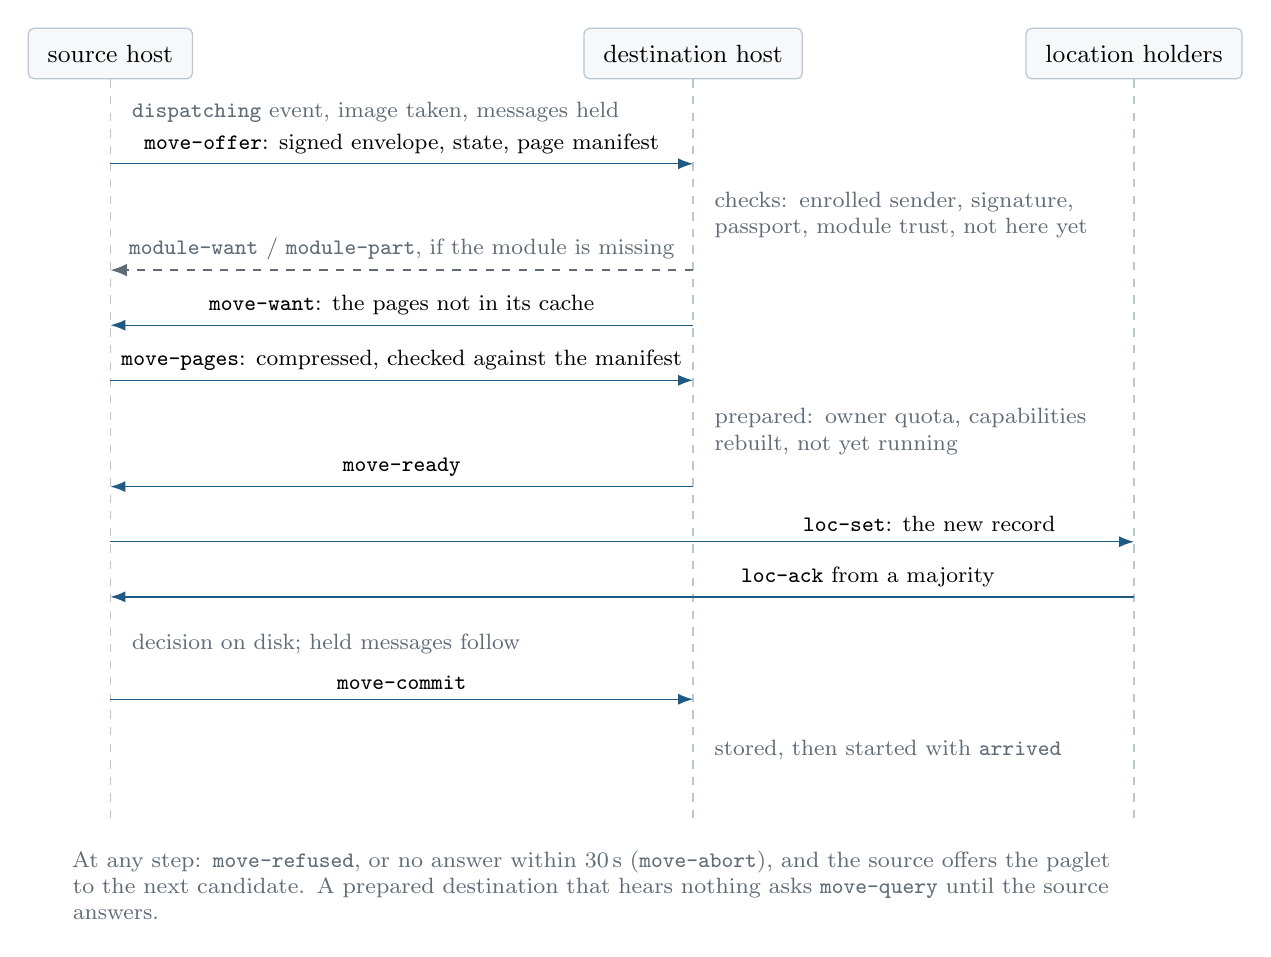
\begin{tikzpicture}[x=1cm,y=1cm]
  \node[box] (S) at (0,0) {source host};
  \node[box] (D) at (7.4,0) {destination host};
  \node[box] (L) at (13.0,0) {location holders};
  \draw[lifeline] (S.south) -- ++(0,-9.4);
  \draw[lifeline] (D.south) -- ++(0,-9.4);
  \draw[lifeline] (L.south) -- ++(0,-9.4);
  \node[event,anchor=west,align=left] at (0.15,-0.75) {\code{dispatching} event, image taken, messages held};
  \draw[msg] (0,-1.4) -- node[above]{\code{move-offer}: signed envelope, state, page manifest} (7.4,-1.4);
  \node[event,anchor=west,align=left,text width=4.9cm] at (7.55,-2.05) {checks: enrolled sender, signature, passport, module trust, not here yet};
  \draw[dashedarrow] (7.4,-2.75) -- node[above,font=\footnotesize,color=pagletsMuted]{\code{module-want} / \code{module-part}, if the module is missing} (0,-2.75);
  \draw[msg] (7.4,-3.45) -- node[above]{\code{move-want}: the pages not in its cache} (0,-3.45);
  \draw[msg] (0,-4.15) -- node[above]{\code{move-pages}: compressed, checked against the manifest} (7.4,-4.15);
  \node[event,anchor=west,align=left,text width=4.9cm] at (7.55,-4.8) {prepared: owner quota, capabilities rebuilt, not yet running};
  \draw[msg] (7.4,-5.5) -- node[above]{\code{move-ready}} (0,-5.5);
  \draw[msg] (0,-6.2) -- node[above,pos=0.8]{\code{loc-set}: the new record} (13.0,-6.2);
  \draw[msg] (13.0,-6.9) -- node[above,pos=0.26]{\code{loc-ack} from a majority} (0,-6.9);
  \node[event,anchor=west,align=left] at (0.15,-7.5) {decision on disk; held messages follow};
  \draw[msg] (0,-8.2) -- node[above]{\code{move-commit}} (7.4,-8.2);
  \node[event,anchor=west,align=left,text width=4.9cm] at (7.55,-8.85) {stored, then started with \code{arrived}};
  \node[event,anchor=north west,align=left,text width=13.6cm] at (-0.6,-10.0) {At any step: \code{move-refused}, or no answer within 30\,s (\code{move-abort}), and the source offers the \paglet{} to the next candidate. A prepared destination that hears nothing asks \code{move-query} until the source answers.};
\end{tikzpicture}
\caption{A move between two hosts. Solid arrows are frames on the encrypted host channels; the dashed one happens only when the destination lacks the module.}
\label{fig:movement-protocol}
\end{figure}

\subsubsection{Departure}

When the handler that called \code{dispatch} returns, the runtime
delivers the \code{dispatching} event, takes the image, and checks that
no pin arrived meanwhile. It then releases the instance and holds every
message that arrives for the \paglet{}; until the mesh reports the
outcome the \paglet{} exists only as its image and record. The node
attaches the \paglet{}'s passport, the signed chain from an enrolled
owner that says who launched it (Section~\ref{sec:mesh}); a \paglet{}
without one does not move (\code{no passport: only paglets of enrolled
owners move}). Before it looks at candidates, the node applies the
residency rule that forbids leaving at all
(Listing~\ref{lst:movement-residency}).

% snippet: cpp/host/src/node/movement.cpp#residency [float,caption={Data that stays on its host keeps the \paglet{} there},label={lst:movement-residency}]
\begin{lstlisting}[style=paglets-cpp,float,caption={Data that stays on its host keeps the \paglet{} there \src{cpp/host/src/node/movement.cpp}},label={lst:movement-residency}]
// Data residency (planning/cpp-residency.md): a paglet that read a root
// whose content stays on this host does not leave.
for (const auto& mark : d.state.marks) {
    if (!mark.starts_with("root:")) continue;
    auto rule = ledger.state().residency.find(mark.substr(5));
    if (rule != ledger.state().residency.end() && rule->second.host_only)
        return fail("data residency: the content of root " + rule->first + " stays on this host");
}
\end{lstlisting}
% /snippet

\subsubsection{The offer and the checks}

The offer is a canonical map: protocol version, mesh, source and
destination keys, request number, kind (\code{dispatch} or \code{clone}),
\paglet{} ID, passport, travelling state, the page manifest (page count,
globals, and per page a hash or nil), the arrival mode, the move counter
after this move, and the time. The source signs the SHA-256 of the body
with its host key under the domain string \code{paglets move offer v1}, so
the destination can check who sent it independent of the channel the
frame came through, which matters for relayed hosts. Before any page
moves, the destination refuses unless everything in
Listing~\ref{lst:movement-accept} holds: the sender is an enrolled host
and the signature verifies, the offer names this host and this mesh, the
state decodes and agrees with the offer, the passport verifies for this
\paglet{} and module (its owner is enrolled and the passport has not
expired; for clones and children, every link is signed by an enrolled
host), the module may run as a roaming \paglet{} in this mesh, and the
\paglet{} is not here already.

% snippet: cpp/host/src/node/movement.cpp#accept [float,caption={What the destination checks before any page moves},label={lst:movement-accept}]
\begin{lstlisting}[style=paglets-cpp,float,caption={What the destination checks before any page moves \src{cpp/host/src/node/movement.cpp}},label={lst:movement-accept}]
if (*mesh_id != ledger.mesh() || *body_from != from || *to != key.public_key() ||
    static_cast<std::uint64_t>(*body_request) != request || (*kind != "dispatch" && *kind != "clone")) {
    return refuse("offer not for this host");
}
auto state = runtime::decode_state(*state_bytes);
if (!state) return refuse(state.error());
auto module = mesh::parse_key_id(state->module);
if (!module || state->id != *paglet) return refuse("offer and state disagree");
auto passport = mesh::Passport::decode(*passport_bytes);
if (!passport) return refuse("passport: " + passport.error());
if (auto ok = mesh::verify_passport(*passport, st, *paglet, *module, mesh::unix_ms()); !ok) {
    return refuse("passport: " + ok.error());
}
if (auto verdict = mesh::check_module(st, *module, "roaming"); !verdict.allowed) return refuse(verdict.reason);
if (runtime.info(*paglet)) return refuse("paglet " + paglet->substr(0, 8) + " is here already");
auto image = parse_image_manifest(*manifest, *module);
if (!image) return refuse("malformed page manifest");
\end{lstlisting}
% /snippet

\subsubsection{The module and the pages}

A destination that lacks the module fetches it by hash: from its module
sources (directories the host was started with), then from the source
host, then from every other host of the mesh, in parts of at most 1\,MB
(\code{need\_module} in \code{cpp/host/src/node/node\_impl.hpp}). Whatever
arrives is verified against the hash and checked as a \paglet{} module
before it is stored; a host that sends something else or does not answer
within 10\,s is skipped for the next. Modules are at most 64\,MB. A host
that still holds the module, because it ran it before or received it with
an earlier move, fetches nothing; a module without a \paglet{} is kept for
24 hours (Section~\ref{sec:movement-code}).

Pages are transferred only when needed. Every host keeps the pages of
images it sent or received in a cache of 256\,MB, least recently used
out, keyed by page hash. The destination compares the manifest against
the cache and asks (\code{move-want}) only for the page indices it lacks;
the source answers with those pages, each compressed with zstd, in frames
of about 1\,MB (a frame is closed once its compressed pages reach that
size). A \paglet{} that returns to a host it visited, or whose
memory changed little since its last move, transfers only the pages that
changed. Every page received is decompressed to exactly 64\,KB and hashed;
a page that does not match the signed manifest ends the arrival
(\code{damaged page}).

With all pages present, the destination prepares the arrival: the runtime
creates the \paglet{} without running it, checks the module's admission
as a roaming \paglet{} and the owner's quota on this host (10\,000
\paglets{} of one owner per host), rebuilds the capability table
(Table~\ref{tab:movement-caps}), re-arms timers and the timeouts of
requests in flight, and keeps the \code{arrived} event ready. Then it
answers \code{move-ready}.

\subsubsection{Commit}

Only the source decides. On \code{move-ready} it first sends the
\paglet{}'s new location record, with the incremented move counter, to the
hosts responsible for it (three of the hosts that are up, chosen by
consistent hashing, or all of them when three or fewer are up,
Section~\ref{sec:communication}) and waits for a majority of
acknowledgements. Then it writes the decision to its state directory,
tells the runtime, and sends \code{move-commit}. The runtime forwards the
held messages to the new host, remembers for ten minutes where the
\paglet{} went (a tombstone, so endpoints with a stale location keep
working), removes the \paglet{}'s record, image and directories, and
reports the outcome to anyone waiting. The destination, on
\code{move-commit}, writes the \paglet{} and its passport to disk at once
and starts it with \code{arrived}, or keeps it stored until a message
comes when the ticket said \code{arrival=inactive}.

The order protects the invariant that a \paglet{} runs on at most one
host. The destination never starts a prepared \paglet{} on its own: when
it hears nothing within the move timeout of 30\,s it asks
\code{move-query}, and keeps asking, and the source answers from its
recorded decisions (kept for an hour) with \code{move-commit} or
\code{move-abort}. A source that crashed after writing the decision
answers the same way when it comes back. If the location records cannot
be updated within the move timeout, the source aborts the move. A
responsible host that answers with a newer record (a counter lost in a
crash) makes the source record again above it, at most three times, and
then abort as well. An aborted move overwrites the records with a higher
counter that names the source: the \paglet{} stays.

\subsubsection{Failure}

The destination may refuse, with the reason (\code{move-refused}), or
stay silent for 30\,s, after which the source sends \code{move-abort};
either moves the offer to the next candidate of the ticket, each offer
with a new request number so late answers do not match. When no candidate is left the move fails; the
runtime makes the \paglet{} ready again with its held messages and
delivers \code{paglets.move\_failed} with the destination it asked for and
the reason of every host tried, such as \code{host lab-2: quota: its
owner has as many paglets here as one owner may have}. Nothing of the
\paglet{} is lost in any of these cases, because the image on the source
is the \paglet{} until the commit.

\subsubsection{From the command line}

An owner or admin moves a \paglet{} with \code{paglets-host remote
dispatch}, which sends the ticket to the host the \paglet{} is on and
waits for the outcome through the same hook the runtime calls at the end
of a move (Listing~\ref{lst:movement-cli}; the session options are those
of Section~\ref{sec:tools-cli}):

\begin{lstlisting}[style=paglets-bash,caption={Moving a \paglet{} from the command line (\code{paglets-host remote}).},label={lst:movement-cli}]
H=paglets-host
S="--connect https://lab-1:7443 --key olga.key --ledger ledger"
ID=$($H remote launch $S build/macos-arm64/guests/journey.wasm)
$H remote dispatch $S $ID lab-2            # moved to lab-2 2f8e1c0b94a7d3e1
$H remote dispatch $S $ID "label:gpu?retries=2"
# the move failed, the paglet stays: no host matches label:gpu
$H remote locate $S $ID                    # host:  lab-2 2f8e1c0b94a7d3e1...
                                           # moves: 1
\end{lstlisting}

\code{remote dispatch} waits at most 120\,s for the outcome and exits
with status 1 and the reason when the move failed.
\code{paglets-web} offers the same move (Section~\ref{sec:tools}).

\subsection{Clones on other hosts}\label{sec:movement-clones}

\code{clone\_raw(args, caps, destination)} makes a copy of the \paglet{}
with the same image, and with a destination the copy is made on another
host. The image is the one taken when the handler returns, so all clones
of one handler call share it; at most 16 children and clones may be made
per call. A remote clone leaves as a departure of its own, with the
clone's ID in the travelling state. It keeps the original's transferable
endpoints and its default service endpoints under the same handle numbers
(so handles in the copied memory stay meaningful), but no requests in
flight; \code{caps} may hold only endpoints to \paglets{} and artifacts,
the capabilities that are meaningful on every host
(\code{invalid\_argument} otherwise). The original continues;
\code{clone\_raw} returns an endpoint
to the clone at once, which reaches it wherever it lands. On the
destination the clone goes through the same offer, checks and commit as a
move, with a passport link that the source host signed to extend the
original's passport, and starts with \code{cloned} (the arguments, the
capabilities and the original's ID) instead of \code{arrived}. If no host
takes it, the original receives \code{on\_move\_failed} with the clone's
ID in \code{MoveFailed::clone}.

The inventory example uses this for a fan-out: one clone per host, each
asks its host's \code{server-info} and reports to the parent. The parent
starts the fan-out with the hosts from \code{mesh-info}'s landscape and
passes a failed clone to the pattern (Listing~\ref{lst:movement-fanout});
the \code{FanOut} pattern of the SDK's patterns library
(\code{patterns/fanout.hpp}) clones the \paglet{} to each destination with
the parent's own endpoint as
the only capability, and arms a timer for the deadline.

% snippet: cpp/examples/inventory/inventory.cpp#fanout [float,caption={The inventory's fan-out},label={lst:movement-fanout}]
\begin{lstlisting}[style=paglets-cpp,float,caption={The inventory's fan-out \src{cpp/examples/inventory/inventory.cpp}},label={lst:movement-fanout}]
    void on_move_failed(const paglets::abi::MoveFailed& f) override {
        if (!f.clone.empty()) fan_.clone_failed(f);
    }

private:
    void start(const Collect& c, Message& m) {
        report_ = Report{};
        auto reply = std::make_shared<paglets::Capability>(m.defer_reply());
        auto go = [this, c, reply](std::vector<std::string> hosts) {
            const auto sent = fan_.start(hosts, paglets::encode(c), c.timeout_ms);
            (void)paglets::reply_to(*reply, Started{sent > 0, sent > 0 ? "" : "no clone went out",
                                                    static_cast<std::int64_t>(hosts.size())});
        };
        if (!c.hosts.empty()) return go(c.hosts);
        auto mi = paglets::service("mesh-info");
        if (!mi) return go({""});
        svc::mesh_info::Client client{*mi};
        auto sent = client.landscape({}, [go](paglets::Result<svc::mesh_info::Landscape> l, Message&) {
            std::vector<std::string> hosts{""};
            if (l) {
                for (std::size_t i = 1; i < l->hosts.size(); ++i) hosts.push_back(l->hosts[i].host);
            }
            go(std::move(hosts));
        });
        if (!sent) go({""});
    }
\end{lstlisting}
% /snippet

A clone finds itself on the new host in \code{on\_cloned}
(Listing~\ref{lst:movement-clone}). Its first capability is the parent's
endpoint; it looks up \code{server-info} on the host it is on, asks it,
reports through the endpoint and disposes itself.

% snippet: cpp/examples/inventory/inventory.cpp#clone [float,caption={A clone on its host},label={lst:movement-clone}]
\begin{lstlisting}[style=paglets-cpp,float,caption={A clone on its host \src{cpp/examples/inventory/inventory.cpp}},label={lst:movement-clone}]
void on_cloned(paglets::Started& s) override {
    Collect q;
    if (s.caps.empty() || !s.decode_args(q)) {
        (void)paglets::dispose();
        return;
    }
    parent_ = paglets::Endpoint(s.caps[0].release());
    query_ = q;
    pt::lookup("server-info", [this](paglets::Result<paglets::Endpoint> ep) {
        if (!ep) return finish(pt::error_text("server-info", ep.error()));
        info_ = *ep;
        summary();
    });
}
\end{lstlisting}
% /snippet

The parent sees each child once, when it reported, when its clone could
not be made or did not arrive, or when the deadline passed without a
report (Listing~\ref{lst:movement-collect}). An inventory is therefore
complete even when a host is down: that host's entry carries the error.

% snippet: cpp/examples/inventory/inventory.cpp#collect [float,caption={Collecting the reports},label={lst:movement-collect}]
\begin{lstlisting}[style=paglets-cpp,float,caption={Collecting the reports \src{cpp/examples/inventory/inventory.cpp}},label={lst:movement-collect}]
fan_.attach(router(), [this](const pt::FanOut::Child& c) {
    HostInventory h;
    if (!c.ok || !paglets::decode(c.result, h)) {
        h = HostInventory{};
        h.error = c.error.empty() ? "no report" : c.error;
    }
    h.host = c.host;
    h.host_name = c.host_name.empty() ? c.destination : c.host_name;
    report_.hosts.push_back(std::move(h));
    report_.finished = fan_.finished();
    if (report_.finished) {
        std::ranges::sort(report_.hosts, [](const auto& a, const auto& b) { return a.host_name < b.host_name; });
    }
});
\end{lstlisting}
% /snippet

\subsection{Deactivation, checkpoints and restarts}\label{sec:movement-disk}

The image that moves a \paglet{} also parks it. \code{deactivate()} takes
effect when the handler returns: the \code{deactivating} event is
delivered, the image is taken, and the instance is released, so an
inactive \paglet{} holds no memory and no compiled code. On a host with a
state directory the image is written to \code{paglets/<id>.paglet}
together with the record, to a temporary file first and then renamed, so
a crash leaves the old file or the new one; without a state directory the
image stays in the host's memory. The next message, timer or wake-up
restores the instance from the image and delivers \code{activated}
before it (Section~\ref{sec:lifecycle-deactivation}).

The same file is the \paglet{}'s checkpoint. With a state directory, the
runtime stores an image after a handler when the last one is older than
the checkpoint interval (1\,s by default, per \paglet{}), at once after
\code{checkpoint()}, and at once when a moved or cloned \paglet{} is
committed, so a crash right after a commit finds the \paglet{} on the
destination. The restart policy of Section~\ref{sec:lifecycle-restart}
(\code{set\_restart(false)}) turns this off.

When a host starts, it reads every \code{.paglet} file and re-creates the
\paglets{} with the restart policy: the record with its capabilities,
timers re-armed for their time, and the image to be restored on the first
delivery (\code{Runtime::Impl::recover} in \code{cpp/host/src/runtime.cpp}).
Requests that were in flight at the crash are answered \code{timeout}, so
the handlers waiting for them run and can retry. A \paglet{} that asked
for it receives \code{recovered} first (Section~\ref{sec:lifecycle}). A
\paglet{} whose module is no longer in the store is dropped with a log
line. A crashed worker process takes the same path for its \paglets{}:
they resume from their last image, except the one whose handler was
running.

\subsection{Code mobility and its limits}\label{sec:movement-code}

Code is named by content. A \paglet{}'s record names its module by SHA-256
hash, the image is bound to that hash, and every host that runs the
\paglet{} holds the module under that hash in its store, verified when it
arrived and again whenever it is read from disk. A module that a host
fetched for one arrival serves every later one; modules without a
\paglet{} are collected after 24 hours. Hosts send modules only to
enrolled hosts.

Whether a module may run is a decision of the mesh, recorded in the
ledger (Section~\ref{sec:mesh}). Signers vouch for a module with a
signature record; admins trust a signer, or a module hash, for the
classes roaming, resident and system; revoking the signer's key, the
signature or the module hash takes the trust back. By default roaming
modules need no trust (\code{module-policy any}); with
\code{module-policy trusted} the destination refuses a module that no
trust record covers before any page moves, and a host ends the
\paglets{} of a module that loses trust while they run. An arriving \paglet{} is always checked as
roaming, whatever it was: resident and system \paglets{} do not move.

Data residency follows the data into the \paglet{}. When a \paglet{} reads
from a named root through the \code{files} service, its host marks it
\code{root:NAME}; the mark is never removed, travels with the \paglet{}
and passes to its children and clones. A residency rule in the ledger
makes the mark bind: \code{host-only} keeps the \paglet{} where it is
(Listing~\ref{lst:movement-residency}: the host where it read, unless
the rule came after a later move), \code{hosts}
limits the candidates of every ticket to the hosts a selector names, by
key or label. A rule made after the read applies, because the mark names
the root, not the rule. The content exchange between hosts obeys the
same rules for artifacts and shared files.

The design has these limits:

\begin{itemize}
\item Only roaming \paglets{} of enrolled owners move, only within one
  mesh, and only to hosts that run the same major and at least the same
  minor ABI version.
\item A \paglet{} never changes code while it lives. The image belongs to
  one module hash; a new version is a new module, and its \paglets{}
  start fresh. There is no state migration between versions.
\item Moves happen between handlers. A computation that takes longer than
  one handler (5\,s) must be split into messages the \paglet{} sends to
  itself, and it can move only between them. This is weak mobility in the
  sense of Section~\ref{sec:background}, by design.
\item A \paglet{} is at most 16\,MB of memory, images included. Larger
  data stays on hosts and travels as artifacts.
\item Capabilities that stand for host resources are re-created only from
  grants; the \code{storage} store and the scratch directory do not
  follow the \paglet{}.
\item The host cannot verify that a module leaves its tables alone; a
  module that does not satisfies the ABI only on paper.
\end{itemize}

Section~\ref{sec:evaluation} measures what these decisions cost: image
sizes, the time to capture and restore an image, the pages a repeated
move sends, moves between two hosts in one process, and the transfer
rates between the hosts of the live mesh. A move between two real
machines is exercised there but not timed.

% Copyright (c) 2026 by C. Klukas.
% Licensed under the MIT License. See LICENSE for details.

A paglet reaches another paglet only through an endpoint, a capability
that names the target by its ID (Section~\ref{sec:model}). The endpoint
does not name a host. This chapter shows how a message still arrives
when its target has moved since the endpoint was handed out, what the
sender sees when it cannot, and what holds a paglet in place while
somebody acts on an answer.

\subsection{Endpoints across hosts}\label{sec:communication-endpoints}

The host of a sending paglet keeps, with every endpoint and reply
capability whose target is on another host, a \emph{host hint}: the key
ID of the host where the target was last known to be (\code{Cap::host} in
the runtime's \code{capability.hpp}; empty for targets on this host).
A capability gets the hint when it leaves a host, in a message or with a
moving paglet. Endpoints to system paglets carry none: they do not travel
in messages, and a moving paglet's endpoints to its default services are
made anew on arrival from the destination's own system paglets
(Section~\ref{sec:movement}). A send, request or reply whose target is not
on this host leaves the runtime as a \code{RemoteMessage} (the runtime's
\code{mobility.hpp}): the target and its hinted host, the message, and
for a request the requester, its host and the correlation. Only endpoints
to paglets travel between hosts, and artifact capabilities (of the
\code{artifacts} system paglet, Section~\ref{sec:mesh}), which name the
host that holds their content. A send, request or reply to a paglet on
another host that carries any other capability is refused with
\code{unsupported}; a message that was accepted on the same host and then
follows its target after a move has such capabilities dropped as
\code{gone}. Lending a capability (\code{SendOptions::lend}) shows it to a
system paglet of this host only; a lend to another host is
\code{invalid\_argument}. The node wraps the message in a \code{deliver}
frame and sends it through the channel to the hinted host
(Section~\ref{sec:communication-channel}).

The hint is a guess. It is right for a target that has not moved. When
it is wrong, the host that receives the frame has to find the target
without help from the sender.

\subsection{Location records}\label{sec:communication-records}

Every paglet has a location record: the host that holds it, its move
counter, when it arrived there and its owner. No host is special. The
records of a paglet live on three \emph{responsible hosts} chosen by
consistent hashing~\cite{karger1997consistent} over the hosts this host
believes are up: each host
has 16 points on a 64-bit ring (SHA-256 over a fixed prefix, the host key
and the point number), a paglet has one point, and the first three
distinct hosts clockwise from it keep its record. With three or fewer
hosts, all of them do (Listing~\ref{lst:comm-responsible}).

% snippet: cpp/host/src/node/location.cpp#responsible [float,caption={The responsible hosts of a paglet: the first three distinct hosts clockwise from its point on the ring},label={lst:comm-responsible}]
\begin{lstlisting}[style=paglets-cpp,float,caption={The responsible hosts of a paglet: the first three distinct hosts clockwise from its point on the ring \src{cpp/host/src/node/location.cpp}},label={lst:comm-responsible}]
std::vector<mesh::PublicKey> Node::Impl::responsible_for(const runtime::PagletId& paglet) {
    update_view();
    if (view.size() <= replicas) return view;
    std::vector<mesh::PublicKey> out;
    const std::uint64_t p = paglet_point(paglet);
    auto it = std::ranges::lower_bound(ring, std::pair{p, mesh::PublicKey{}});
    for (std::size_t n = 0; n < ring.size() && out.size() < replicas; ++n, ++it) {
        if (it == ring.end()) it = ring.begin();
        if (std::ranges::find(out, it->second) == out.end()) out.push_back(it->second);
    }
    return out;
}
\end{lstlisting}
% /snippet

Creation writes a record with counter~0. Every move increments the
counter, and a record with a higher counter replaces one with a lower
counter; the same counter from the same host only refreshes it. The
counter is what makes a stale record harmless: a host that was down and
returns with an old record loses to any newer one. The update is the
commit step of the move protocol (Section~\ref{sec:movement-protocol}):
the source sends the new record to the responsible hosts and commits the
move only after a majority ($\lfloor n/2 \rfloor + 1$) acknowledged it,
recording above a newer record at most three times before it aborts and
the paglet stays. So every committed move is visible to a majority of
the responsible hosts before the paglet runs on its new host.

The set of live hosts changes. Every host sends a heartbeat to every
enrolled host every 2\,s (any frame counts as one); a host not heard from
for 10\,s, or one that announced another mesh protocol or ABI version, is
out of this host's view, and the ring is rebuilt over the view. Holders
then re-send the records of their paglets, and every host sends the
records it keeps to hosts that became responsible for them. Holders also
refresh their records every five minutes, and a record not refreshed for
an hour ends, which removes the records of paglets that ended. Records are
kept in the node's state directory, so a restarted host still has them.
Different hosts can disagree about the view for a few seconds; the lookup
below has a fallback for the case that no responsible host knows a paglet.

\subsection{Delivery after a move}\label{sec:communication-delivery}

A lookup (the node's lookup behind \code{Node::locate}, the
\code{locator} system paglet, \code{paglets-host remote locate} and
message forwarding) runs in three steps, the second and third limited to
3\,s each. First, a paglet on this host is found at once. Second, the
responsible hosts are asked (\code{loc-get}); with answers from a
majority, the record with the highest counter wins, which is the latest
committed location. When the 3\,s pass with fewer answers, the best record
that did arrive is used, which may be stale. Third, if no responsible host
knows the paglet, every live host is asked (\code{loc-who}), and the host
that holds it answers; if none does, the lookup ends with
\code{not\_found}. Hosts cache the answers of lookups and moves for 10\,s.

Message forwarding adds a cheaper first step. A host remembers for ten
minutes where a departed paglet went (a \emph{tombstone},
\code{Config::tombstone\_ttl}). A message that arrives for a paglet that
left is forwarded to the tombstone's host, with a hop counter in the
message that allows at most four forwards in all. Only when the host has
neither the paglet nor a tombstone, and the message has not yet been
forwarded four times, does the runtime hand the message to the node
(\code{MobilityHooks::unresolved}), which uses its location cache or
starts a lookup and forwards the message to the host it finds
(Listing~\ref{lst:comm-unresolved}). A request that nobody holds is
answered \code{not\_found} to the requester; a one-way message that
nobody holds is dropped. Figure~\ref{fig:comm-forward} shows both paths.

% snippet: cpp/host/src/node/location.cpp#unresolved [float,caption={Messages for paglets that are neither here nor remembered: the location cache, otherwise a lookup; requests for paglets nobody holds are answered},label={lst:comm-unresolved}]
\begin{lstlisting}[style=paglets-cpp,float,caption={Messages for paglets that are neither here nor remembered: the location cache, otherwise a lookup; requests for paglets nobody holds are answered \src{cpp/host/src/node/location.cpp}},label={lst:comm-unresolved}]
for (auto& m : queue) {
    auto deliver = [this](runtime::RemoteMessage& msg, const mesh::PublicKey& host) {
        msg.host = mesh::key_id(host);
        ++msg.hops;
        send_remote(std::move(msg));
    };
    if (auto c = loc_cache.find(m.target); c != loc_cache.end() && Clock::now() - c->second.second < cache_ttl &&
                                           c->second.first.host != key.public_key()) {
        deliver(m, c->second.first.host);
        continue;
    }
    Lookup l;
    l.kind = LookupKind::locate;
    l.paglet = m.target;
    l.done = [this, m = std::move(m), deliver](const LookupResult& r) mutable {
        if (r.status == abi::ok) return deliver(m, r.where.host);
        if (m.kind != runtime::RemoteMessage::Kind::request) return;
        // Nobody has it: the requester hears so.
        runtime::RemoteMessage answer;
        answer.kind = runtime::RemoteMessage::Kind::reply;
        answer.target = m.requester;
        answer.host = m.requester_host;
        answer.correlation = m.correlation;
        answer.status = abi::not_found;
        send_remote(std::move(answer));
    };
    start_lookup(std::move(l));
}
\end{lstlisting}
% /snippet

\begin{figure}[htbp]
\centering
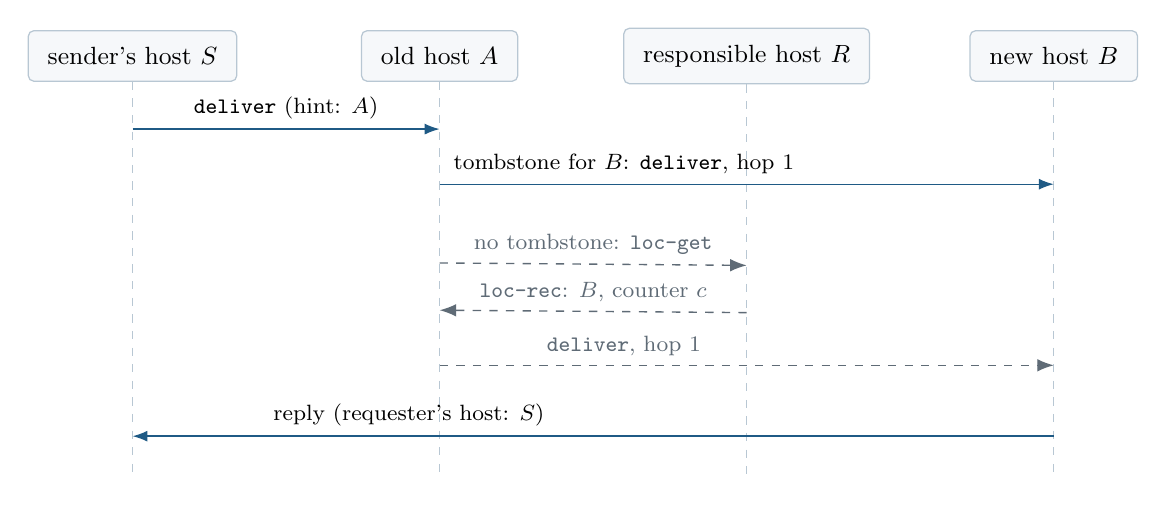
\begin{tikzpicture}[x=1cm,y=1cm]
  \node[box] (s) at (0,0) {sender's host $S$};
  \node[box] (a) at (3.9,0) {old host $A$};
  \node[box] (r) at (7.8,0) {responsible host $R$};
  \node[box] (b) at (11.7,0) {new host $B$};
  \foreach \n in {s,a,r,b} \draw[lifeline] (\n.south) -- ++(0,-5.0);
  \draw[msg] ($(s.south)+(0,-0.6)$) -- node[above]{\code{deliver} (hint: $A$)} ($(a.south)+(0,-0.6)$);
  \draw[msg] ($(a.south)+(0,-1.3)$) -- node[above,pos=0.3]{tombstone for $B$: \code{deliver}, hop $1$} ($(b.south)+(0,-1.3)$);
  \draw[dashedarrow] ($(a.south)+(0,-2.3)$) -- node[above,event]{no tombstone: \code{loc-get}} ($(r.south)+(0,-2.3)$);
  \draw[dashedarrow] ($(r.south)+(0,-2.9)$) -- node[above,event]{\code{loc-rec}: $B$, counter $c$} ($(a.south)+(0,-2.9)$);
  \draw[dashedarrow] ($(a.south)+(0,-3.6)$) -- node[above,event,pos=0.3]{\code{deliver}, hop $1$} ($(b.south)+(0,-3.6)$);
  \draw[msg] ($(b.south)+(0,-4.5)$) -- node[above,pos=0.7]{reply (requester's host: $S$)} ($(s.south)+(0,-4.5)$);
\end{tikzpicture}
\caption{A request to a paglet that moved from $A$ to $B$ after the sender got its endpoint. $A$ forwards by its tombstone (solid), or, after the tombstone ended or $A$ restarted, by a lookup on the responsible hosts (dashed). The reply goes to the requester's host directly, because a request names it.}
\label{fig:comm-forward}
\end{figure}

A paglet in the middle of a move handles no message: after the handler
that called \code{dispatch} it receives only the \code{dispatching} event,
and from then until the outcome is known the runtime holds the messages
that arrive for it. When the move succeeds, the held messages are sent on
to the new host in mailbox order (by priority, then arrival); a held
request becomes a remote request that names the requester and its host,
so its reply finds the way back. When the move fails, the paglet
continues on its host and handles the held messages there. In the other
direction, the paglet's own requests in flight travel with it: the
travelling state lists each pending correlation with its remaining time,
and the new host arms the timeouts again on arrival. The continuation of
a request lives in the paglet's memory and moves with the image, so a
reply that arrives after the move runs the continuation on the new host.
Table~\ref{tab:comm-timing} collects the constants of this section.

\begin{table}[htbp]
\centering\small
\caption{Timing and limits of location and delivery. Names without a file are fields of \code{Node::LocationTiming} (\code{node.hpp}). All are compiled-in defaults; the node's timings can be changed by its embedder, not from the command line.}
\label{tab:comm-timing}
\begin{tabular}{llll}
\toprule
Quantity & Value & Name & File \\
\midrule
Heartbeat to every enrolled host & 2\,s & \code{heartbeat} & \\
A host counts as down after & 10\,s & \code{host\_timeout} & \\
Lookup steps two and three & 3\,s each & \code{lookup\_timeout} & \\
Location cache & 10\,s & \code{cache\_ttl} & \code{location.cpp} \\
Record refresh by holders & 5\,min & \code{refresh} & \\
A record not refreshed ends after & 1\,h & \code{record\_ttl} & \\
Tombstone of a departed paglet & 10\,min & \code{Config::tombstone\_ttl} & \code{runtime.hpp} \\
Forwards of one message & 4 & \code{max\_forwards} & \code{runtime.cpp} \\
Redirects a pin follows & 8 & \code{max\_hops} & \code{location.cpp} \\
Waits for a moving paglet & $40 \times 100$\,ms & \code{max\_busy}, \code{busy\_wait} & \code{location.cpp} \\
Default request timeout & 30\,s & \code{abi::default\_timeout\_ms} & \code{abi.hpp} \\
Mailbox of a paglet & 1024 messages & \code{Config::mailbox\_limit} & \code{runtime.hpp} \\
\bottomrule
\end{tabular}
\end{table}

\subsection{Pins}\label{sec:communication-pins}

An answer from the locator can be stale by the time its receiver acts on
it. A \emph{pin} keeps a paglet on its host for a while. While a paglet
holds an unexpired pin, its own \code{dispatch} returns \code{pinned}
(error $-17$), and a dispatch an owner or admin requests is refused with
the same error. A dispatch requested before the pin fails with
\code{paglets.move\_failed} when it comes due.
\code{self\_info().pinned\_until} names the end of its last pin. Cloning,
deactivation and messages are not affected. A paglet can hold up to 64
pins and moves once all have ended. Pins are leases: they end at their
expiry, when their holder releases them or when an admin ends them
(\code{remote unpin}). The node stores them in its state and applies them
again after a restart. A pin never races a move: pinning a paglet that is
leaving or about to leave is refused with \code{bad\_state}, and the pin
protocol then waits 100\,ms and looks the paglet up again; a host that no
longer has the paglet redirects the pin to its tombstone's host. One
counter bounds both: a pin ends with \code{timeout} after eight redirects,
or after 40 waits and redirects together.

Paglets pin through the \code{locator} system paglet, whose endpoint
every paglet has by default (operations \code{locate},
\code{locate\_and\_pin} and \code{release}). The caller lends the
endpoint of the target, which must carry the \code{locate} or \code{pin}
right. \code{locate\_and\_pin} finds the paglet and pins it where it is in
one step; its reply carries the \code{Location} (paglet ID, host key ID
and name, time of the last move, move counter), the pin's ID and end, and
as its first capability a \emph{pin capability} of kind \code{pin} with
the right \code{release}. The capability is transferable and stays valid
when its holder moves; releasing revokes it and every copy. Who may pin,
and for how long, is decided by the mesh policy: \code{locate\_and\_pin}
needs a rule that allows service \code{locator}, operation \code{pin},
for the caller, and the rule's \code{max\_duration\_ms} caps the pin (one
hour without a maximum; the request itself is clamped to between 1\,s and
30 days). Without such a rule, pinning is \code{denied}. Owners (for their
own paglets) and admins pin through a CLI session (\code{paglets-host
remote pin}), which needs no rule: 10 minutes by default, at most 24
hours.

The Hide and Seek example (\code{cpp/examples/seek/}) plays this out
under continuous movement. The hider is a child that moves to \code{any}
host on a timer; while pinned, its \code{dispatch} says so at once and it
tries again later (Listing~\ref{lst:comm-hider}).

% snippet: cpp/examples/seek/seek.cpp#hider [float,caption={The hider moves on a timer and treats a refused dispatch as a reason to try later},label={lst:comm-hider}]
\begin{lstlisting}[style=paglets-cpp,float,caption={The hider moves on a timer and treats a refused dispatch as a reason to try later \src{cpp/examples/seek/seek.cpp}},label={lst:comm-hider}]
    void on_created(paglets::Started& s) override {
        // Created by a seeker: hide (args: the hop interval).
        if (!s.decode_args(hop_ms_) || hop_ms_ <= 0) return;
        hiding_ = true;
        (void)paglets::after_raw(hop_ms_, "hop", {});
    }

    void on_arrived(const paglets::abi::ArrivedEvent&) override {
        if (!hiding_) return;
        ++moves_;
        (void)paglets::after_raw(hop_ms_, "hop", {});
    }

    void on_move_failed(const paglets::abi::MoveFailed&) override {
        if (hiding_) (void)paglets::after_raw(hop_ms_, "hop", {});  // pinned, or nowhere to go: later
    }

private:
    // -- the hider ----------------------------------------------------------------------

    void hop() {
        if (!hiding_) return;
        // While pinned, dispatch says so at once: try again later.
        if (!paglets::dispatch("any")) (void)paglets::after_raw(hop_ms_, "hop", {});
    }
\end{lstlisting}
% /snippet

The seeker keeps one endpoint to the hider. Each round it pins the hider
for at most 10\,s with \code{patterns::with\_pinned}
(\code{<paglets/patterns/locate.hpp>}), which calls
\code{locate\_and\_pin}, runs the work with the location, and releases
the pin when the work calls \code{done}. Pinned, the hider answers the
request \code{moves} from the host where it was found, which is the point
of the pin: the answer and the location belong to the same host
(Listing~\ref{lst:comm-seek}). A round starts only once the hider has
moved since the last catch, so every catch finds it after a new move.
Table~\ref{tab:comm-seek} records the test on three hosts in one process,
with a hop every 30\,ms.

% snippet: cpp/examples/seek/seek.cpp#seek [float,caption={A round of Hide and Seek: pin the hider where it is, ask it something there, let it go},label={lst:comm-seek}]
\begin{lstlisting}[style=paglets-cpp,float,caption={A round of Hide and Seek: pin the hider where it is, ask it something there, let it go \src{cpp/examples/seek/seek.cpp}},label={lst:comm-seek}]
// The next round starts once the hider has moved since the last catch,
// however slow the hosts are.
void round() {
    if (static_cast<std::int64_t>(score_.catches.size()) >= game_.rounds) return finish();
    hider_moves([this](std::int64_t n) {
        if (!score_.catches.empty() && n >= 0 && n <= caught_at_moves_) {
            (void)paglets::after_raw(game_.pause_ms, "next-round", {});
            return;
        }
        seek();
    });
}

void seek() {
    pt::with_pinned(hider_, 10'000, "hide and seek",
                    [this](paglets::Result<pt::Location> where, std::function<void()> done) {
                        Catch c;
                        if (where) {
                            c.host_name = where->host_name;
                            c.moves = where->moves;
                        } else {
                            c.error = std::string(paglets::abi::error_name(where.error()));
                        }
                        score_.catches.push_back(std::move(c));
                        // Pinned, it stays where it is while it counts.
                        hider_moves([this, done](std::int64_t n) {
                            caught_at_moves_ = n;
                            done();  // let it go
                            (void)paglets::after_raw(game_.pause_ms, "next-round", {});
                        });
                    });
}
\end{lstlisting}
% /snippet

% Hand-written from docs/results/seek.json (recorded 2026-10-12): the
% `% results: seek` marker renders every column of the JSON (test name,
% outcome, platform, date, ...), which is wider than the text block; see
% the refinement plan. Keep these numbers in step with the JSON.
\begin{table}[htbp]
\centering\small
\caption{Hide and Seek on three hosts in one test process (\code{example: Hide and Seek finds and pins a paglet that keeps moving}, Darwin arm64, Release build, recorded 2026-10-12): four rounds with a hop every 30\,ms and 300\,ms between rounds. Both runs passed.}
\label{tab:comm-seek}
\begin{tabular}{lrrr}
\toprule
Mode & Duration (s) & Catches & Moves of the hider \\
\midrule
in-process & 1.7 & 4 & 35 \\
worker processes & 1.8 & 4 & 30 \\
\bottomrule
\end{tabular}
\end{table}

\subsection{Asynchronous sends, replies and failures}\label{sec:communication-async}

\code{Endpoint::send} and \code{Message::reply} are synchronous by
default: the call returns when the host has accepted the message, with
\code{denied}, \code{expired} or \code{quota} when the endpoint does not
allow it, \code{not\_found} when a target on this host ended, and
\code{quota} when the target's mailbox here is full. For a target on
another host the call succeeds once the runtime has handed the message to
the node; whether the frame reaches the other host is not reported. The
remote host answers a request that it cannot deliver (unknown paglet, full
mailbox, a system paglet of its own) with the error as the reply status,
and drops a one-way message it cannot deliver.

With \code{SendOptions::async}, \code{reply\_async} or \code{async = true}
in \code{reply\_to}, the call returns \code{ok} as soon as the document is
well-formed. This matters in worker processes (Section~\ref{sec:model}):
a synchronous call is a round trip to the host, an asynchronous one is a
one-way frame. A failure is reported later as the host's report
\code{paglets.undelivered}, which the SDK delivers to
\code{on\_undelivered} with the name, the handle and the error the
synchronous call would have returned; transferred capabilities are gone
and a failed reply has answered the requester \code{gone}
(Section~\ref{sec:lifecycle-reports}). A request is never
asynchronous: \code{RequestOptions} has no \code{async}, and the ABI call
refuses the flag with \code{invalid\_argument}, since a request has its
continuation. Its timeout (\code{RequestOptions::timeout\_ms}, 30\,s by
default) runs on the requester's host and is armed again after a move;
when it passes, the continuation runs with status \code{timeout}, and a
reply that arrives later is discarded.

Ping Pong (Listings~\ref{lst:pingpong-roles} and \ref{lst:pingpong-bounce})
has both sides: the child answers with \code{reply\_async}, the parent
answers a deferred reply from the continuation of the last ping or drops
it, which answers the caller \code{gone} at once. Nothing in it depends on
where the child is: had the child dispatched itself between two pings,
the parent's endpoint would carry the next ping to it by the paths of
Section~\ref{sec:communication-delivery}. The example in the repository
stays on one host; Hide and Seek above and the Latency Map below talk
across hosts.

\subsection{Hosts without an inbound port}\label{sec:communication-relays}

A host behind NAT or a firewall can open connections but accept none.
Started with \code{--no-listen}, such a host keeps two \emph{relays},
reachable hosts that it polls for the frames held for it (the
transport's \code{poll} request), and announces them to the mesh in place
of an address; the bootstrap contact of \code{--join} is the first. Every
other host reaches it through a relay over a Noise channel of its own,
tunneled in transport control frames, so the relay sees only the two host
keys and the sizes. Relaying is a duty of every reachable host. The design
is in \code{planning/cpp-relay.md}; the test \code{host\_mesh\_discovery}
runs a host with \code{--no-listen} that joins through another and
receives a paglet.

\subsection{The channel between hosts}\label{sec:communication-channel}

Hosts talk HTTPS, and inside it Noise channels~\cite{perrin2018noise}
(\code{Noise\_XX\_25519\_ChaChaPoly\_SHA256}, built on libsodium). The
static keys of the handshake are the X25519 forms of the Ed25519 identity
keys, so the peer of a channel is an identity key, which the node checks
against the ledger (Section~\ref{sec:mesh}). The prologue contains the
mesh ID, so hosts of different meshes fail at the second handshake
message. TLS keeps proxies and firewalls working and authenticates
nothing by itself: a host checks the certificates of the hosts it
connects to only when it was started with \code{-{}-tls-ca FILE}; the
identity of a peer is its Noise key in every case. A server handles the
requests of a session one at a time, so
frames arrive in the order they were sent. Frames that cannot be delivered
are dropped and counted; the protocols above time out: a lookup asks the
records once more and then fails, a move offers the next host of its
ticket or is aborted, and the paglet stays.

\subsection{Measuring the links}\label{sec:communication-latency}

The Latency Map (\code{cpp/examples/latency/}) measures what a request
between paglets on two hosts costs. It clones a probe to every host; each
probe derives an endpoint to itself that allows only \code{ping},
\code{probe.peers} and \code{probe.done} and sends it to the parent, which
hands every probe copies of the others' endpoints narrowed to
\code{ping}. A probe pings its targets one at a time, waits for each
reply before the next ping and keeps the shortest and the mean round
trip per target (Listing~\ref{lst:comm-ping}); a ping without a reply in
5\,s puts the status into the cell. The parent collects one row per
probe with the \code{FanOut} pattern and then tells the probes to end.

% snippet: cpp/examples/latency/latency.cpp#ping [float,caption={A probe of the Latency Map pings one target at a time and records the round trip in the continuation},label={lst:comm-ping}]
\begin{lstlisting}[style=paglets-cpp,float,caption={A probe of the Latency Map pings one target at a time and records the round trip in the continuation \src{cpp/examples/latency/latency.cpp}},label={lst:comm-ping}]
// Pings target `t`, round `round`; one at a time.
void ping(std::size_t t, std::int64_t round) {
    if (t >= targets_.size()) {
        for (auto& x : targets_) {
            if (x.cell.replies > 0) x.cell.avg_ms /= static_cast<double>(x.cell.replies);
            row_.cells.push_back(x.cell);
        }
        return pt::report(parent_, paglets::encode(row_));
    }
    if (round >= rounds_) return ping(t + 1, 0);
    const double sent_at = now_ms();
    paglets::RequestOptions o;
    o.timeout_ms = 5000;
    auto sent = targets_[t].endpoint.request(
        "ping",
        [this, t, round, sent_at](Message& reply) {
            Cell& c = targets_[t].cell;
            if (reply.ok()) {
                const double rtt = now_ms() - sent_at;
                c.avg_ms += rtt;
                c.min_ms = c.replies == 0 ? rtt : std::min(c.min_ms, rtt);
                ++c.replies;
            } else {
                c.error = std::string(paglets::abi::error_name(reply.status()));
            }
            ping(t, round + 1);
        },
        std::move(o));
    if (!sent) {
        targets_[t].cell.error = pt::error_text("ping", sent.error());
        ping(t + 1, 0);
    }
}
\end{lstlisting}
% /snippet

Table~\ref{tab:comm-latency} is the last run on real machines: the live
mesh of Section~\ref{sec:evaluation-setup}, a Mac Studio (\emph{mac}), a
Raspberry Pi~4 (\emph{pi}) and a uConsole built on a Raspberry Pi
Compute Module~5 (\emph{uconsole}) on a gigabit LAN, 20 pings per pair,
with the probes in worker processes. A round trip passes both runtimes,
the worker process boundary on both sides and the encrypted channel
between the hosts; relays would add to it. The evaluation
(Section~\ref{sec:evaluation-mesh}) puts the numbers next to the TCP
baseline and the transfer rates of the same mesh.

% Hand-written from docs/results/live_latency.json (recorded 2026-10-12):
% the `% results: live_latency` marker renders every column of the JSON
% (mode, outcome, build, date, ...), which is wider than the text block;
% see the refinement plan. Keep these numbers in step with the JSON.
\begin{table}[htbp]
\centering\small
\caption{Round trips of a request between probes on two hosts (mac: Mac Studio; pi: Raspberry Pi~4; uconsole: uConsole on a Raspberry Pi Compute Module~5), gigabit LAN, probes in worker processes, Release build, 20 pings per pair, recorded 2026-10-12.}
\label{tab:comm-latency}
\begin{tabular}{lrr}
\toprule
Pair & Mean of 20 (ms) & Fastest (ms) \\
\midrule
mac $\rightarrow$ pi & 2.84 & 1.08 \\
mac $\rightarrow$ uconsole & 4.69 & 1.92 \\
pi $\rightarrow$ mac & 4.07 & 1.71 \\
pi $\rightarrow$ uconsole & 1.34 & 0.79 \\
uconsole $\rightarrow$ mac & 5.16 & 1.83 \\
uconsole $\rightarrow$ pi & 1.16 & 0.79 \\
\bottomrule
\end{tabular}
\end{table}

\section{Mesh Policies and Compute Jobs}\label{sec:mesh}
% Copyright (c) 2026 by C. Klukas.
% Licensed under the MIT License. See LICENSE for details.

A mesh is a set of hosts that trust the same signed ledger. Nothing else
binds them: there is no central server, no shared secret, and no
membership list or policy outside the ledger. This section describes the ledger and the identities
in it, the passports that paglets carry, the policy that decides access to
host resources, the system paglets through which that access is given, the
contracts that define them, and the two services with which a paglet sees
the mesh and gets compute time on it. Figure~\ref{fig:mesh} shows the
parts.

\begin{figure}[htbp]
\centering
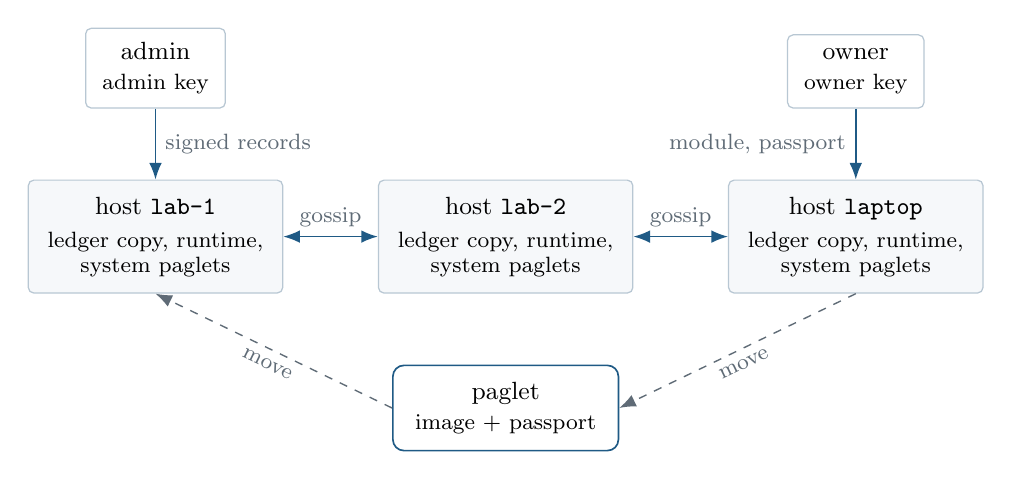
\begin{tikzpicture}[node distance=9mm and 12mm]
  \node[box] (h1) {host \code{lab-1}\\[1pt]\footnotesize ledger copy, runtime,\\[-2pt]\footnotesize system paglets};
  \node[box, right=of h1] (h2) {host \code{lab-2}\\[1pt]\footnotesize ledger copy, runtime,\\[-2pt]\footnotesize system paglets};
  \node[box, right=of h2] (h3) {host \code{laptop}\\[1pt]\footnotesize ledger copy, runtime,\\[-2pt]\footnotesize system paglets};
  \draw[both] (h1) -- node[event, above] {gossip} (h2);
  \draw[both] (h2) -- node[event, above] {gossip} (h3);
  \node[plain, above=of h1] (admin) {admin\\\footnotesize admin key};
  \draw[arrow] (admin) -- node[event, right] {signed records} (h1);
  \node[plain, above=of h3] (owner) {owner\\\footnotesize owner key};
  \draw[arrow] (owner) -- node[event, left] {module, passport} (h3);
  \node[state, below=of h2] (p) {paglet\\\footnotesize image + passport};
  \draw[dashedarrow] (h3.south) -- node[event, below, sloped] {move} (p.east);
  \draw[dashedarrow] (p.west) -- node[event, below, sloped] {move} (h1.south);
\end{tikzpicture}
\caption{A mesh of three hosts. Every host holds a copy of the ledger and
  enforces the state it derives from it. Gossip spreads ledger records
  and host announcements; every host sends its own snapshot to every live
  host. An admin signs records on its own
  machine and brings them to any live host. An owner signs a passport for
  a paglet it launches; the passport moves with the paglet's image.}
\label{fig:mesh}
\end{figure}

\subsection{Hosts and the ledger}\label{sec:mesh-ledger}

Identities are Ed25519 keys in four roles: admins, hosts, owners and
signers (signers vouch for modules, Section~\ref{sec:movement}). A key's
ID is the hex form of its public key. Admin, owner and signer keys are
stored encrypted with a passphrase (Argon2id, XChaCha20-Poly1305); host
keys are stored unencrypted with owner-only file permissions, because a
host starts without a person.

The ledger is a grow-only set of signed records. A record is a canonical
MessagePack body with a set of signatures. Its ID is the SHA-256 of the
body, and signatures cover the ID, so a signature can be added later
without changing the record: this is how several admins co-sign a record
that needs a quorum. The first record is the genesis record: the mesh
name, the initial admins and the quorum, two numbers: how many admin
signatures an admin record needs, and how many a change of the admin set
needs (both 1 unless \code{mesh create} is given \code{-{}-quorum} and
\code{-{}-admin-quorum}; \code{admin-set} records change them). Its ID
is the mesh ID, with which a host opens its ledger copy as its trust
anchor.
Table~\ref{tab:ledger-records} lists the record types.

\begin{table}[htbp]
\centering\small
\begin{tabular}{@{}p{4.9cm}p{3.6cm}p{5.6cm}@{}}
\toprule
Record & Signed by & Content \tabularnewline
\midrule
\raggedright\code{genesis} & \raggedright every initial admin & \raggedright mesh name, admins, quorum \tabularnewline
\raggedright\code{admin-set} & \raggedright the admin-set quorum of its epoch & \raggedright admins added or removed, quorum \tabularnewline
\raggedright\code{host-enroll-request}, \code{owner-enroll-request} & \raggedright the key itself & \raggedright key, name; a host's labels \tabularnewline
\raggedright\code{host-enroll}, \code{owner-enroll} & \raggedright admin quorum & \raggedright key, name, labels (host) or groups (owner), the request answered \tabularnewline
\raggedright\code{host-remove}, \code{owner-remove} & \raggedright admin quorum & \raggedright key \tabularnewline
\raggedright\code{request-deny}, \code{revoke} & \raggedright admin quorum & \raggedright a request; a key, a record or a module \tabularnewline
\raggedright\code{module-sign} & \raggedright a signer & \raggedright module hash, name, version \tabularnewline
\raggedright\code{module-trust}, \code{module-policy} & \raggedright admin quorum & \raggedright modules or signers per trust class; whether roaming modules need trust \tabularnewline
\raggedright\code{root-residency} & \raggedright admin quorum & \raggedright where the content of a named root may go \tabularnewline
\raggedright\code{policy-rule} & \raggedright admin quorum & \raggedright decision, service, operations, match, scope \tabularnewline
\raggedright\code{grant-request} & \raggedright the paglet's host, or the owner & \raggedright principal, items, duration, reason \tabularnewline
\raggedright\code{grant} & \raggedright admin quorum, or a host under an allow rule & \raggedright principal, item, hosts, expiry \tabularnewline
\raggedright\code{grant-release}, \code{audit} & \raggedright a host & \raggedright a released grant; a decision \tabularnewline
\bottomrule
\end{tabular}
\caption{The ledger's record types (\code{cpp/host/include/paglets/mesh/ledger.hpp}).
  Records of unknown types are kept and replicated but have no effect, so
  newer record types pass through older hosts.}
\label{tab:ledger-records}
\end{table}

Adding a record checks only its form, its signatures and its mesh. What a
record means is decided when the state is derived from the whole set, in a
fixed order: by Lamport clock, then by ID. Hosts that hold the same
records derive the same state, whatever order the records arrived in.
Three rules close the gaps that a signed set leaves open. Admin changes
form a chain of epochs, and a signature counts only if its signer was an
admin of the epoch the record names. Because the signer chooses the
clock, the record that removes an admin lists the records that admin had
signed so far (its keep list); the removed admin's signatures count only
on those, so whatever it signs later, with any epoch and clock, has no
effect. Revocations win regardless of order: a revoked key is removed and
can never be enrolled again, and a revoked record has no effect. Records
without effect are listed with the reason (\code{LedgerState::ignored}),
and a digest of the derived state compares two hosts.

Replication is gossip over the host channels. A record that is new to a
host goes on at once to every host it knows except the sender; periodic
anti-entropy rounds exchange digests and inventories and repair what the
pushes missed. Every host holds the whole ledger and enforces the last
state it has, so allow and deny rules keep working while the mesh is
partitioned or no admin is online; when the partition heals, the records
merge. The ledger has no checkpoints yet: a host's copy grows with every
record.

A new host or owner signs an enrollment request with its own key, as proof
of possession, and an admin approves it from any host or enrolls the key
directly. An admin works on a local ledger copy and brings its records to
a live host with \code{remote push}; from there they spread. A host whose
key is not enrolled yet starts anyway and waits for its enrollment record.
Hosts find each other through a bootstrap contact (\code{--join URL}),
through signed host announcements that spread like records, and on a
local network through multicast beacons. A channel between two hosts
proves both host keys against the ledger, is encrypted end to end inside
HTTPS, and is refused between hosts of different mesh protocol versions or
paglet ABI major versions. Listing~\ref{lst:mesh-cli} builds a small
mesh: an admin creates it, enrolls a host and an owner, and adds a rule
under which the paglets of owners in the group \code{staff} must ask
before they read below \code{docs/} of the named root \code{data}; the
host binds that root to a directory when it starts
(\code{--root data=/srv/data}). The grant requests that such paglets later
make under the rule (Section~\ref{sec:mesh-policy}) are what
\code{remote requests} lists and \code{remote approve} decides;
\code{ledger audit} prints every decision the local copy holds.

\begin{lstlisting}[style=paglets-bash,float,caption={A mesh with one host and one owner, and a policy rule.},label={lst:mesh-cli}]
H=build/macos-arm64/host/paglets-host
$H keys init --role admin --name alice --out alice.key
$H keys init --role host --name lab-1 --out lab-1.key       # prints <lab-1-key-id>
$H keys init --role owner --name olga --out olga.key        # prints <olga-key-id>
$H mesh create --name lab --ledger ledger --admin alice.key
$H ledger enroll --ledger ledger --admin alice.key host <lab-1-key-id> lab-1 --label linux
$H ledger enroll --ledger ledger --admin alice.key owner <olga-key-id> olga --group staff
$H ledger rule --ledger ledger --admin alice.key --name "staff docs" --decision ask \
    --service files --op read --group staff --root data --path "docs/**"
$H serve --key lab-1.key --ledger ledger --state state-1 --listen 0.0.0.0:7443 \
    --advertise https://lab-1:7443 --root data=/srv/data
$H remote requests --connect https://lab-1:7443 --key alice.key --ledger ledger
$H remote approve  --connect https://lab-1:7443 --key alice.key --ledger ledger <request-id>
$H ledger audit --ledger ledger
\end{lstlisting}

\subsection{Passports}\label{sec:mesh-passports}

A paglet carries a passport. Its root is signed by the owner's key: the
mesh, the owner, the module hash, the paglet ID, a capability manifest,
and the issue and expiry times. \code{remote launch} issues one on the
owner's machine, valid for 24 hours unless \code{--hours} says otherwise,
and sends it to the host with the module and the start arguments. A child
or clone extends its creator's passport with a link signed by the host
that created it: the kind (\code{child} or \code{clone}), the parent and
the new paglet ID, the new module hash, the creating host, the issue
time, and the hash of the previous element, so a link cannot be moved to
another chain. A host verifies a
passport when it creates the paglet and when the paglet arrives from
another host: the signatures and the chain, the mesh, that the owner and
every linking host are enrolled and not revoked, that the passport has
not expired, and that its last element names the paglet and module in
question. The passport is stored beside the paglet and moves with its
image.

From the passport and the module the host forms the \emph{principal} that
every policy decision is made for: the paglet ID, the owner, the module
hash and the trust class (\code{roaming}, \code{resident} or
\code{system}). The host stamps the same fields into the sender record of
every delivered message, so a receiver can rely on them without a check
of its own. The manifest, a list of policy items the paglet declares in
advance, is evaluated by the same rules. The ledger accepts an
owner-signed \code{grant-request} for a paglet ID chosen in advance, so an
admin can approve the manifest before the paglet exists, and the grants
materialize when the paglet starts. No command of \code{paglets-host}
issues such a request yet, and \code{remote launch} issues passports with
an empty manifest.

\subsection{Policy rules and grants}\label{sec:mesh-policy}

Access to host resources is decided by rules in the ledger. The unit of
access is an \emph{item}: a service and its operations, and for
\code{files} a named root and a path below it, with rights (\code{read},
\code{write}, \code{create}, \code{delete}) in place of operations. A rule
names a service (or \code{*}) and operations, a decision (\emph{allow},
\emph{ask} or \emph{deny}), a match on the principal and the host, and for
files a scope. The match selects owners, owner groups, module hashes,
module signers, trust classes, and hosts by key or label; an absent member
matches everything. The scope lists roots and path patterns (\code{*},
\code{?}, \code{**}). A rule can bound the duration of the grants it gives
and carry a priority.

A host evaluates an item for a principal from its own ledger copy. Among
the rules that match the principal and the host, name the service and
cover all the operations and the scope, the most specific one wins:
highest priority, then most match members, then a scope over none, then
\emph{deny} over \emph{ask} over \emph{allow}, then ledger order. When no
rule matches, the decision is \emph{deny}. Every host evaluates the same
rules, so the decision does not depend on which host a paglet is on, only
on the host selectors of the rules.

The decision becomes records. Under an \emph{allow} rule the host signs a
\code{grant} that names the rule and itself as the only host; it expires
after the requested duration (1~s to 30 days), capped by the rule's
maximum. Other hosts accept such a grant only if the rule allows it for
that principal, so a host cannot mint access its rules do not give. Under
an \emph{ask} rule the host signs a \code{grant-request}; it is pending
until an admin, from any host, signs a \code{grant} that names it (with
\code{remote approve}, for every host or only the requesting one) or a
\code{request-deny}. A \emph{deny} leaves only the audit record. Every
decision writes an \code{audit} record signed by the host, and the admin's
approvals, denials and revocations are records themselves, so the audit
log is the ledger and is read from any host (\code{remote audit};
\code{ledger audit} prints the audit records a local copy holds). A grant
ends when it expires, when an admin revokes it, or when a host releases
it.

A paglet asks through the \code{grants} system paglet
(Listing~\ref{lst:grants-request}). The answer is \code{granted}, with the
capability as the first capability of the reply; \code{pending}, with the
request ID; or \code{denied}, with the deciding rule, if any. When an
approval arrives by gossip, the paglet's host \emph{materializes} the grant
and sends the capability in the message \code{grants.granted}
(Figure~\ref{fig:grant-flow}); a denial arrives as \code{grants.denied}. A
files item becomes a \code{dir} capability for the root and path with the
rights, the grant's ID and its expiry; an item of another service becomes
a non-transferable endpoint carrying the granted operations. The
capability records its grant, and the runtime refuses it with
\code{revoked} as soon as the record that revokes or releases the grant
arrives: every copy, derivative and transfer of the capability fails on
every host. An admin's grant belongs to the mesh, not to a host: it
materializes on every host its selector covers, also when the paglet
arrives there later, so it follows the paglet, while a host-local
capability does not (Section~\ref{sec:movement}). A grant a host derived
from an \emph{allow} rule names that host only; after a move the paglet
asks again, and the same rule allows again.

% snippet: cpp/common/include/paglets/services/grants.hpp#request [float,caption={The request and the answer of the \code{grants} service},label={lst:grants-request}]
\begin{lstlisting}[style=paglets-cpp,float,caption={The request and the answer of the \code{grants} service \src{cpp/common/include/paglets/services/grants.hpp}},label={lst:grants-request}]
struct Item {
    std::string service;           // files, server-info, ...
    std::vector<std::string> ops;  // files: rights (read, write, create, delete)
    std::string root;              // files: named root
    std::string path;              // files: directory below the root ("" for the root)
};

struct Request {
    Item item;
    std::int64_t duration_ms = 3'600'000;
    std::string reason;
};

enum class Status { granted, pending, denied };

struct Answer {
    Status status = Status::denied;
    Item item;
    std::string grant;    // hex ID of the grant record (granted)
    std::string request;  // hex ID of the request record (pending, and later answers)
    std::string rule;     // hex ID of the deciding rule, if any
    std::int64_t expires_ms = 0;
    std::string reason;
};
\end{lstlisting}
% /snippet

\begin{figure}[htbp]
\centering
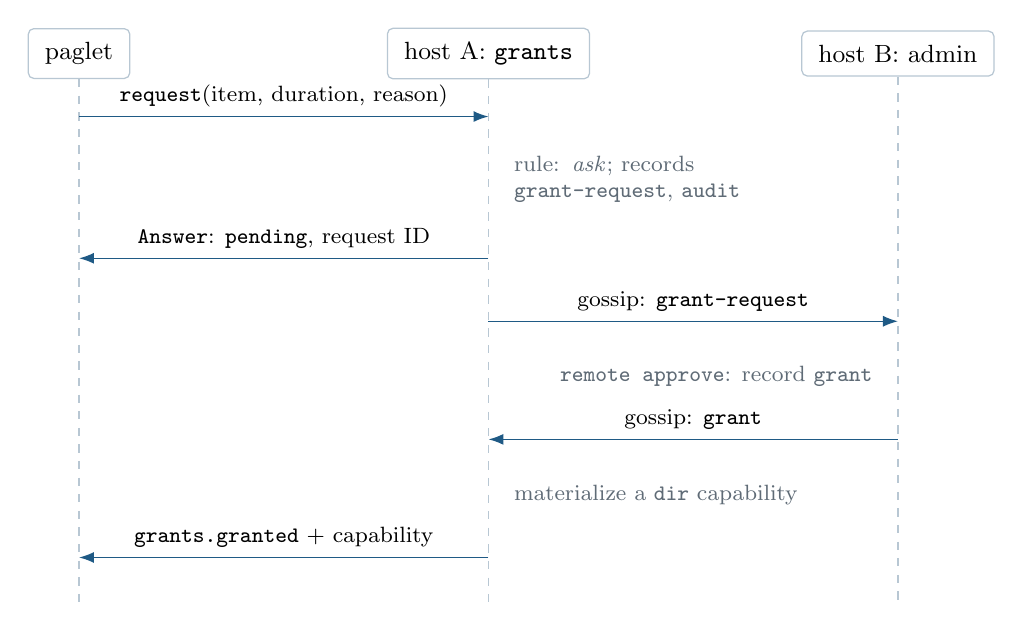
\begin{tikzpicture}[x=1cm,y=1cm]
  \node[plain] (P) at (0,0) {paglet};
  \node[plain] (A) at (5.2,0) {host A: \code{grants}};
  \node[plain] (B) at (10.4,0) {host B: admin};
  \draw[lifeline] (P.south) -- (0,-7.0);
  \draw[lifeline] (A.south) -- (5.2,-7.0);
  \draw[lifeline] (B.south) -- (10.4,-7.0);
  \draw[msg] (0,-0.8) -- node[above] {\code{request}(item, duration, reason)} (5.2,-0.8);
  \node[event, anchor=west, align=left, text width=4.4cm] at (5.4,-1.6) {rule: \emph{ask}; records\\\code{grant-request}, \code{audit}};
  \draw[msg] (5.2,-2.6) -- node[above] {\code{Answer}: \code{pending}, request ID} (0,-2.6);
  \draw[msg] (5.2,-3.4) -- node[above] {gossip: \code{grant-request}} (10.4,-3.4);
  \node[event, anchor=east] at (10.2,-4.1) {\code{remote approve}: record \code{grant}};
  \draw[msg] (10.4,-4.9) -- node[above] {gossip: \code{grant}} (5.2,-4.9);
  \node[event, anchor=west] at (5.4,-5.6) {materialize a \code{dir} capability};
  \draw[msg] (5.2,-6.4) -- node[above] {\code{grants.granted} + capability} (0,-6.4);
\end{tikzpicture}
\caption{A grant request under an \emph{ask} rule. The admin decides on
  any host; the records travel by gossip; the paglet's host turns the
  approval into a capability.}
\label{fig:grant-flow}
\end{figure}

The pi example of Section~\ref{sec:mesh-compute} writes its digits below a
named root of its host. It asks for the directory with the patterns
helper \code{granted\_dir}, which sends the request and hands the
capability to a continuation (Listing~\ref{lst:pi-grant}). The helper
treats \code{pending} as a failure (\code{bad\_state}); a paglet that wants
to wait for an admin handles \code{grants.granted} itself.

% snippet: cpp/examples/pi/pi.cpp#grant [float,caption={The pi job asks for a directory of the named root it was started with},label={lst:pi-grant}]
\begin{lstlisting}[style=paglets-cpp,float,caption={The pi job asks for a directory of the named root it was started with \src{cpp/examples/pi/pi.cpp}},label={lst:pi-grant}]
pt::granted_dir(s.output_root, "", {"write", "create"}, "pi: digits", [this](paglets::Result<paglets::Capability> d) {
    if (!d) return fail(pt::error_text("files of " + params_.output_root, d.error()));
    dir_ = std::make_shared<paglets::Capability>(*d);
    const auto slash = params_.output_path.rfind('/');
    pt::make_dirs(*dir_, slash == std::string::npos ? std::string() : params_.output_path.substr(0, slash),
                  [this](paglets::Result<void> made) {
                      if (!made) return fail(pt::error_text("directory for " + params_.output_path, made.error()));
                      begin();
                  });
});
\end{lstlisting}
% /snippet

\subsection{System paglets}\label{sec:mesh-system-paglets}

A paglet runs in a sandbox: it cannot open files, create sockets or start
programs. Hosts lend them such resources through \emph{system paglets},
native services built into the host process. A system paglet is a paglet
for everybody else: it has the ID \code{system.<name>}, a mailbox, and
handles one message at a time; but it has no Wasm instance and no memory
image, and it never deactivates, moves or ends. Its handlers are trusted
host code without a time budget. Besides the ABI's imports
(Appendix~\ref{app:abi}: messages, capabilities, children and the
lifecycle, timers, the clock, random bytes and the log), these services
are the only way a paglet reaches anything on its host.
Table~\ref{tab:system-paglets} lists them.

\begin{table}[htbp]
\centering\small
\begin{tabular}{@{}l p{2.1cm} p{4.4cm} p{5.3cm}@{}}
\toprule
Service & Endpoint & Operations & Purpose \tabularnewline
\midrule
\code{files} & directory & \raggedright\code{list}, \code{stat}, \code{find}, \code{read}, \code{write}, \code{mkdir}, \code{move}, \code{remove}, \code{hash}, \code{share}, \code{save} & \raggedright files below a lent \code{dir} capability; \code{share} and \code{save} move files of any size between hosts as artifacts \tabularnewline
\code{grants} & default & \raggedright\code{request}, \code{status}, \code{release}, \code{list} & \raggedright access by the mesh policy \tabularnewline
\code{storage} & default & \raggedright\code{get}, \code{put}, \code{remove}, \code{list} & \raggedright the paglet's own key-value store, 16~MB \tabularnewline
\code{artifacts} & directory & \raggedright\code{put}, \code{get}, \code{stat} & \raggedright content-addressed blobs (SHA-256) that work on every host \tabularnewline
\code{pubsub} & directory & \raggedright\code{create}, \code{publish}, \code{subscribe}, \code{unsubscribe} & \raggedright topics on a host, reached by \code{topic} capabilities \tabularnewline
\code{server-info} & directory & \raggedright\code{summary}, \code{load}, \code{volumes}, \code{processes} & \raggedright the host's system, in one schema on every platform \tabularnewline
\code{directory} & default & \raggedright\code{lookup}, \code{publish}, \code{unpublish}, \code{list} & \raggedright services and paglets by name \tabularnewline
\code{user-info} & default & \raggedright\code{notify} & \raggedright notifications to the owner \tabularnewline
\code{locator} & default & \raggedright\code{locate}, \code{locate\_and\_pin}, \code{release} & \raggedright a paglet anywhere in the mesh; pins \tabularnewline
\code{mesh-info} & default & \raggedright\code{snapshot}, \code{landscape}, \code{select}, \code{find\_offers} & \raggedright every host's snapshot and offers \tabularnewline
\code{compute-slots} & default & \raggedright\code{request\_slot}, \code{release\_slot}, \code{status}, \code{candidates} & \raggedright admission of compute work \tabularnewline
\code{zombies} & default & \raggedright\code{join}, \code{peers}, \code{trace}, \code{ended}, \code{state}, \code{deliver}, \code{result}, \code{cancel}, \code{redirect}, \code{list}, \code{traces} & \raggedright the host's registry of zombie groups (Section~\ref{sec:zombies}) \tabularnewline
\code{web} & \raggedright directory, \code{--web} hosts & \raggedright\code{capabilities}, \code{fetch}, \code{extract\_text}, \code{download}, \code{search} & \raggedright mediated web access; downloads become artifacts \tabularnewline
\code{ai} & \raggedright directory, \code{--ai} hosts & \raggedright\code{capabilities}, \code{summarize}, \code{classify}, \code{extract}, \code{generate}, \code{embed}, \code{describe\_image} & \raggedright local inference through Ollama \tabularnewline
\bottomrule
\end{tabular}
\caption{The system paglets. \emph{Default}: every paglet is created with a
  non-transferable endpoint to the service. \emph{Directory}: a paglet looks
  the service up. For \code{server-info} the endpoint carries only the
  operations the policy allows; \code{files}, \code{artifacts} and
  \code{pubsub} act only on lent capabilities and need no policy;
  \code{web} and \code{ai} check the policy per request, against rules for
  the URL's host and path, or for the operation and the model.
  Every service also answers \code{describe} with its schema.}
\label{tab:system-paglets}
\end{table}

A paglet reaches a service in one of two ways. Services that act only on
the caller's own things (\code{directory}, \code{storage},
\code{user-info}, \code{grants}, \code{locator}, \code{mesh-info},
\code{compute-slots}, \code{zombies}) are installed as default endpoints
when the paglet is created (\code{paglets::service(name)} returns them).
Services that act only on capabilities the caller lends (\code{files},
\code{artifacts}, \code{pubsub}) are looked up in the \code{directory},
which returns an endpoint with every operation. Neither kind needs a
policy, because holding the capability is the permission.
\code{server-info} has ambient authority: it reads host state without any
capability. It is reached through the \code{directory}, and the endpoint
that a lookup returns carries only the operations the policy allows the
principal; the lookup fails with \code{denied} when it allows none. The
gateways \code{web} and \code{ai} are looked up the same way but decide
per request, against rules whose root and path are the URL's host and
path, or whose operation and scope name the task and the model. The
volume guard example works with \code{server-info}: a rule allows its
owner's paglets the operation \code{volumes}, and the guard looks the
service up, asks for the volumes and notifies its owner when one runs low
(Listing~\ref{lst:guard-check}). The first two calls of the listing
matter here: \code{lookup} returns the endpoint the policy allows, and
\code{volumes} succeeds only because the rule names that operation;
without the rule the lookup fails with \code{denied}. The rest is the
guard's bookkeeping of what it has reported.

% snippet: cpp/examples/guard/guard.cpp#check [float,caption={The volume guard reads the host's volumes through an endpoint whose operations the policy chose},label={lst:guard-check}]
\begin{lstlisting}[style=paglets-cpp,float,caption={The volume guard reads the host's volumes through an endpoint whose operations the policy chose \src{cpp/examples/guard/guard.cpp}},label={lst:guard-check}]
void check() {
    pt::lookup("server-info", [this](paglets::Result<paglets::Endpoint> ep) {
        if (!ep) return failed(pt::error_text("server-info", ep.error()));
        si::Client c{*ep};
        auto sent = c.volumes({}, [this](paglets::Result<si::Volumes> v, Message&) {
            if (!v) return failed(pt::error_text("volumes", v.error()));
            ++status_.checks;
            for (const auto& vol : v->volumes) {
                if (vol.total == 0) continue;
                const double free = 100.0 * static_cast<double>(vol.available) / static_cast<double>(vol.total);
                if (free >= watch_.min_free_percent) {
                    low_.erase(vol.mount_point);  // recovered
                    continue;
                }
                if (!low_.insert(vol.mount_point).second) continue;  // reported already
                status_.alerts.push_back(Alert{vol.mount_point, free, now_ms()});
                pt::notify(pt::Level::warning, "volume " + vol.mount_point + " is low on space",
                           std::to_string(static_cast<int>(free)) + "% free");
            }
            sleep();
        });
        if (!sent) failed(pt::error_text("volumes", sent.error()));
    });
}
\end{lstlisting}
% /snippet

Resource capabilities are the second half of the mechanism. A \code{dir}
capability names a root and a relative path and carries rights, and
optionally the grant it came from, an expiry and a use limit
(Section~\ref{sec:model-capabilities}). The guest never names a host
path: it lends the capability with a request to \code{files}, which acts
on what it is shown and never on its own authority; this is the
confused-deputy protection. A derived capability keeps the lineage and
the grant of its root, so one revocation reaches them all.
\code{files} resolves every path canonically
and refuses one that leads out of the root, also through symbolic links.
Content larger than a message travels as \emph{artifact} capabilities: a
few bytes that name the content by hash and the host that holds it. The
content moves from host to host only when a host needs it, within the
data residency of its root.

\subsection{Service contracts}\label{sec:mesh-contracts}

The system services are contracts of the form of
Section~\ref{sec:model-schemas}: a schema header in
\path{cpp/common/include/paglets/services/}, served on the host by
\code{services::ContractPaglet} and called from a guest through the
generated \code{Client}. Listings~\ref{lst:compute-types}
and~\ref{lst:compute-contract} show the request, the reply and the
contract of \code{compute-slots}.

% snippet: cpp/common/include/paglets/services/compute_slots.hpp#types [float,caption={The request and the reply of \code{request\_slot}},label={lst:compute-types}]
\begin{lstlisting}[style=paglets-cpp,float,caption={The request and the reply of \code{request\_slot} \src{cpp/common/include/paglets/services/compute\_slots.hpp}},label={lst:compute-types}]
struct SlotRequest {
    std::string job;  // the job it belongs to (for status)
    std::int64_t cores = 1;
    std::int64_t estimated_ms = 0;
};

enum class Verdict { run_now, queued, redirect, rejected };

struct Decision {
    Verdict verdict = Verdict::rejected;
    std::string lease;  // run_now
    std::int64_t cores = 0;
    std::string host;           // redirect: key ID of the host to go to
    std::string host_name;      // its name
    std::int64_t position = 0;  // queued: place in the queue (0: next)
    std::string reason;
};
\end{lstlisting}
% /snippet

% snippet: cpp/common/include/paglets/services/compute_slots.hpp#contract [float,caption={The contract of the \code{compute-slots} service},label={lst:compute-contract}]
\begin{lstlisting}[style=paglets-cpp,float,caption={The contract of the \code{compute-slots} service \src{cpp/common/include/paglets/services/compute\_slots.hpp}},label={lst:compute-contract}]
struct Contract {
    static constexpr std::string_view service = "compute-slots";
    Decision request_slot(const SlotRequest&);
    ReleaseReply release_slot(const ReleaseRequest&);
    Status status(const StatusRequest&);
    Candidates candidates(const CandidatesRequest&);
};
\end{lstlisting}
% /snippet

Host and guest embed the same JSON descriptor of the namespace,
byte-identical by construction, and every service answers \code{describe}
with it. (The forms of the tools in Section~\ref{sec:tools} come from a
module's interface description, a separate document that travels inside
the module.) A module names the services it uses in its build rule
(\code{paglets\_add\_module(... SERVICES compute\_slots mesh\_info)}) and
includes \code{<paglets/services/compute\_slots.gen.hpp>}; a caller
cannot tell a guest that serves a contract from a native system paglet.
Contracts need reflection on the host; a host built without it runs
paglets but has no services and no mesh.

\subsection{Mesh information and compute slots}\label{sec:mesh-compute}

Two services let a paglet see the mesh and get compute time on it.
\code{mesh-info} spreads a \emph{snapshot} of every host. Each host
samples itself every 2~s (CPUs, load average per CPU, CPU use, memory,
free space where it keeps state, paglets, compute slots, labels, offers,
and its links to the other hosts: up or down, since when, and why frames
fail) and sends the snapshot to every live host. A host accepts a snapshot
only from the host it describes, over the channel that proved its key; a
snapshot older than 20~s is not fresh, and after a minute it is dropped.
So every host answers for the whole mesh: \code{landscape} lists the hosts
with a fresh snapshot, \code{select} returns the hosts that fit a load,
memory, free-slot and label requirement, the best first, or, when none
fits, the least loaded hosts marked as a fallback, and
\code{find\_offers} the hosts whose services offer a feature, such as
\code{ai.summarize} with a model of a given context size. Offers are also
destinations: a transfer ticket \code{offer:ai.summarize}
(Table~\ref{tab:movement-tickets}) moves a paglet to such a host.

\code{compute-slots} is admission. A host has slots, by default one per
CPU (\code{serve --slots N} changes it); there is no central scheduler or
job queue, every host decides for itself and tells the others what it has
free. A job paglet asks the \code{compute-slots} of the host it is on and
gets a \code{Decision}: \code{run\_now} with a lease when slots are free
and nobody waits; \code{redirect} with a host that has free slots now and
no queue; \code{queued} with its position otherwise; \code{rejected} for
more cores than the host has, unless another host has them free now,
which is a \code{redirect}. The queue is served oldest-fit: the first
waiter, from the oldest, whose cores are free receives the message
\code{compute.granted}, which activates it if it deactivated while
waiting; a small waiter can pass a larger one ahead of it. Waiters behind
the first that have waited a second are offered to hosts that have free
slots and no queue (\code{compute.redirect}, at most four per round and
half the queue, with shadow reservations so that one host is not
flooded). The service never
moves a paglet: the paglet dispatches itself and asks again on arrival. A
lease ends when it is released, or when the paglet ends or leaves the
host.

Listing~\ref{lst:pi-worker} is a worker of the pi example, which computes
hexadecimal digits of pi in independent chunks, each in a clone of the job
on a host that \code{mesh-info} selected. The worker asks for one slot and
acts on the verdict; on a host without the service it runs at once. It
handles \code{compute.granted} by running and \code{compute.redirect} by
dispatching itself; \code{on\_arrived} asks again, and
\code{on\_move\_failed} asks the host it is still on. The job keeps the
state of every chunk and sends a chunk out again when it is not answered
in time, so the loss of a host costs only the chunks in flight there
(Section~\ref{sec:evaluation} reports a live run on three machines, and
the example's test, in which one of three hosts in one process is shut
down mid-run).

% snippet: cpp/examples/pi/pi.cpp#worker [float,caption={A pi worker asks its host for a compute slot},label={lst:pi-worker}]
\begin{lstlisting}[style=paglets-cpp,float,caption={A pi worker asks its host for a compute slot \src{cpp/examples/pi/pi.cpp}},label={lst:pi-worker}]
void ask_for_slot() {
    auto slots = paglets::service("compute-slots");
    if (!slots) return compute();  // a host without compute-slots: just run
    svc::compute_slots::Client client{*slots};
    svc::compute_slots::SlotRequest q;
    q.job = "pi";
    q.cores = 1;
    auto sent = client.request_slot(q, [this](paglets::Result<svc::compute_slots::Decision> d, Message&) {
        if (!d) return compute();
        switch (d->verdict) {
            case svc::compute_slots::Verdict::run_now: run(d->lease); break;
            case svc::compute_slots::Verdict::queued: break;  // compute.granted comes later
            case svc::compute_slots::Verdict::redirect:
                if (!paglets::dispatch(d->host)) compute();
                break;
            case svc::compute_slots::Verdict::rejected: compute(); break;
        }
    });
    if (!sent) compute();
}
\end{lstlisting}
% /snippet

% Copyright (c) 2026 by C. Klukas.
% Licensed under the MIT License. See LICENSE for details.

A paglet is reached by messages whose names and payload types are fixed in
its source. Tools and people who do not read that source need the same
facts in a form a host can read without running the module. This chapter
describes that form, the interface description, and the programs that use
it: the command line \code{paglets-host}, the web UI \code{paglets-web},
and the generator that keeps the documentation and this paper true to the
sources.

\subsection{Interface descriptions}\label{sec:tools-interfaces}

An interface description says which messages a paglet understands, which
types their payloads and replies have, and which arguments it is started
with. It is a JSON document in a Wasm custom section named
\code{paglets.interface}, so it travels inside the module. Custom sections
are part of the module's bytes: the module hash and the ledger's module
signatures (Section~\ref{sec:mesh}) cover the description, and a host reads
it from the bytes it already stores, without instantiating anything.
Listing~\ref{lst:counter-interface} is the description of the counter
example.

% snippet: cpp/examples/counter/interface.json [float,caption={The counter's interface description},label={lst:counter-interface}]
\begin{lstlisting}[style=paglets-json,float,caption={The counter's interface description \src{cpp/examples/counter/interface.json}},label={lst:counter-interface}]
{
  "interface": 1,
  "name": "counter",
  "summary": "A counter whose state is plain C++ objects; memory images move it",
  "launch": {"type": "Start", "example": {"value": 0}},
  "messages": [
    {"name": "increment", "kind": "both", "summary": "Adds to or multiplies the value; replies with the status",
     "request": "Increment", "reply": "Status", "example": {"by": 1, "note": "from the web", "mode": "add"}},
    {"name": "status", "kind": "call", "summary": "The value and the latest notes", "request": "none", "reply": "Status"},
    {"name": "echo", "kind": "call", "summary": "Returns the record unchanged (every field type)", "request": "Echo", "reply": "Echo"},
    {"name": "bloat", "kind": "call", "summary": "Keeps the given amount of memory (image size experiments)",
     "request": "Bloat", "reply": "Status"},
    {"name": "log", "kind": "both", "summary": "Writes a line to the host's log", "request": "string", "reply": "Status"},
    {"name": "schema", "kind": "call", "summary": "The schema descriptor of the messages (JSON text)", "request": "none", "reply": "string"}
  ],
  "types": [
    {"name": "Start", "kind": "record", "fields": [
      {"name": "value", "type": "i64", "doc": "The value to begin with", "default": 0}]},
    {"name": "Increment", "kind": "record", "fields": [
      {"name": "by", "type": "i64", "doc": "Amount (or factor)", "default": 1},
      {"name": "note", "type": "string", "doc": "Kept in the history"},
      {"name": "mode", "type": "Mode", "default": "add"}]},
    {"name": "Bloat", "kind": "record", "fields": [
      {"name": "kilobytes", "type": "u32", "doc": "Memory to keep, in KB", "default": 1024},
      {"name": "fill", "type": "u8", "doc": "Byte value written into it"}]}
  ]
}
\end{lstlisting}
% /snippet

The members are few. \code{interface} is the format version, \code{1}.
\code{launch.type} names the type of the start arguments, or \code{none};
\code{launch.example} fills a launch form. Each entry of \code{messages}
has the name the paglet's router handles, a \code{kind} (\code{call}, a
request with a reply; \code{send}, one-way; or \code{both}; the default is
\code{call}), the \code{request} and \code{reply} types (\code{none} for an
empty payload), one line of \code{summary}, and optionally an
\code{example} payload and \code{danger}, which makes \code{paglets-web} ask
before it sends the message. Names that begin with \code{paglets.} are
reserved. Types are the names of the schema generator
(Section~\ref{sec:model-schemas}): \code{bool}, the integers \code{i8}
to \code{u64}, \code{f32}, \code{f64}, \code{string}, \code{bytes},
\code{list<T>}, \code{optional<T>}, \code{any} for a free JSON value, and
the records and enums listed under \code{types}. Records encode as
MessagePack maps keyed by field name and enums as the enumerator's name,
which are the encodings of the generated codecs, so a description matches
the C++ types of the schema header (Section~\ref{sec:model}).

The description is not the schema. The schema header is the source of the
types; the description adds what the types do not say: the message names,
their kinds, summaries, examples, and per field a \code{doc} and a
\code{default}. The counter's file therefore defines only \code{Start},
\code{Increment} and \code{Bloat}, the records whose fields it documents.
\code{Status}, \code{Echo} and the enum \code{Mode} come from the schema
when the module is built: \code{paglets\_add\_module} takes
\code{INTERFACE counter/interface.json} next to \code{SCHEMA\_HEADER}, and
after linking it runs the interface tool, \code{paglets-interface}, on the
module (Figure~\ref{fig:interface-flow}). The tool merges the records and enums of the generated
\code{counter.schema.json} into \code{types} (a type the description
defines itself takes precedence), checks the result and writes the
section. A description that names an unknown type, repeats a message or
uses another kind fails the build with the reason. A module whose schema
namespace holds service contracts (Section~\ref{sec:mesh}) needs no file:
the tool makes a description with one \code{call} message per operation.
Because embedding changes the module's bytes, a module is signed and
trusted after it was built, as any module is.

\begin{figure}[htbp]
\centering
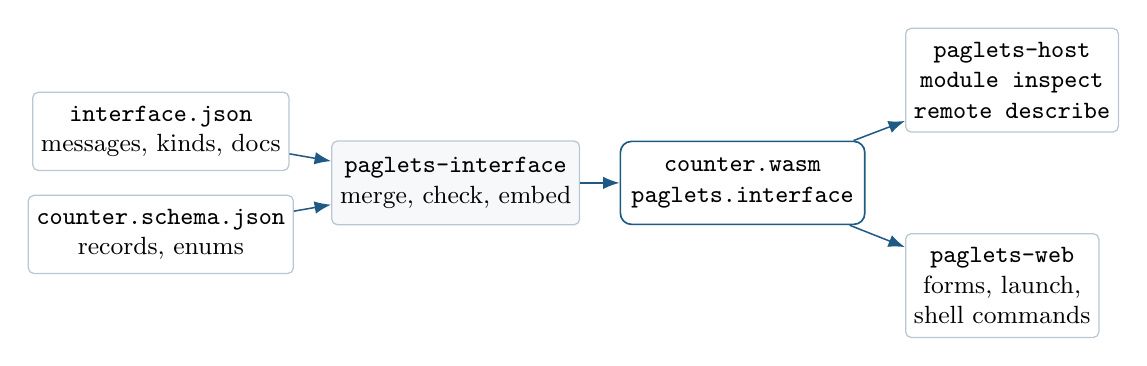
\begin{tikzpicture}[every node/.append style={font=\footnotesize},
                    box/.append style={inner xsep=3pt}, plain/.append style={inner xsep=3pt},
                    state/.append style={inner xsep=4pt}]
  \node[plain] (json) {\code{interface.json}\\messages, kinds, docs};
  \node[plain, below=3mm of json] (schema) {\code{counter.schema.json}\\records, enums};
  \coordinate (mid) at ($(json.east)!0.5!(schema.east)$);
  \node[box, right=5mm of mid] (tool) {\code{paglets-interface}\\merge, check, embed};
  \node[state, right=5mm of tool] (module) {\code{counter.wasm}\\\code{paglets.interface}};
  \node[plain, above right=1mm and 5mm of module] (cli) {\code{paglets-host}\\\code{module inspect}\\\code{remote describe}};
  \node[plain, below right=1mm and 5mm of module] (web) {\code{paglets-web}\\forms, launch,\\shell commands};
  \draw[arrow] (json) -- (tool);
  \draw[arrow] (schema) -- (tool);
  \draw[arrow] (tool) -- (module);
  \draw[arrow] (module) -- (cli);
  \draw[arrow] (module) -- (web);
\end{tikzpicture}
\caption{From the description and the schema's types (written by the schema generator) into the module at build time, and out of the module into the tools. The section is covered by the module hash and the ledger's module signatures. Hosts read it from the stored bytes; the paglet never runs for it.}
\label{fig:interface-flow}
\end{figure}

In the host tree the description is a small API of the \code{wire} library
over the module bytes, which the interface tool links as well
(Listing~\ref{lst:interface-api}). \code{of\_module} finds and parses the
section; \code{validate} is the check the build runs; \code{from\_schema}
builds the generated description of a contract guest. The same code
answers the \code{describe} request of a remote session, also for the
native system paglets, whose descriptions are built from their service
contracts.

% snippet: cpp/host/include/paglets/wire/interface.hpp#api [float,caption={The host's view of interface descriptions},label={lst:interface-api}]
\begin{lstlisting}[style=paglets-cpp,float,caption={The host's view of interface descriptions \src{cpp/host/include/paglets/wire/interface.hpp}},label={lst:interface-api}]
// Checks a description: the format version, message names and kinds, and
// that every type it names is a built-in type or one of its `types`.
std::expected<void, std::string> validate(const Json& description);

// Parses and validates a description given as JSON text.
std::expected<Json, std::string> parse(std::string_view text);

// Adds the records and enums of a schema descriptor (wire/schema.hpp,
// <name>.schema.json) that the description does not define itself.
Json merge_schema_types(Json description, const Json& schema);

// A description made from a schema descriptor's services: one `call`
// message per operation.
Json from_schema(const Json& schema, std::string_view name);

// The interface of a module's bytes: the custom section, parsed; nullopt
// when the module has none.
std::expected<std::optional<Json>, std::string> of_module(std::span<const std::uint8_t> wasm);
\end{lstlisting}
% /snippet

The build checks that every type the description names exists, in the
file or in the schema, and nothing against the paglet's router: a message
the file lists but no handler takes is found when it is sent, by the
\code{unknown\_message} error reply, not by the build. The router keeps
its handlers in a map by name but exposes neither the map nor the names,
so a test cannot compare the two directly; it could only send each
described message and watch for \code{unknown\_message}. The end-to-end
test of \code{paglets-web} launches the counter with a start value, reads
its description and exercises three of its messages (a send and two
calls); beyond that, a description written by hand is as true as its
author keeps it.

\subsection{The command line}\label{sec:tools-cli}

\code{paglets-host} is one program with four groups of commands
(Table~\ref{tab:cli-groups}). The first group runs paglets on one machine
without a mesh, and so without keys or a ledger. The second manages keys
and the signed ledger of a mesh, and inspects module files, all offline.
\code{serve}
runs a host. \code{remote} talks to a running host.

\begin{table}[htbp]
\centering\small
\begin{tabular}{@{}lll@{}}
\toprule
Group & Commands & Works on \\
\midrule
local & \code{run}, \code{list}, \code{call} & a module file or a state directory here \\
records & \code{keys}, \code{mesh create}, \code{ledger}, \code{module inspect} & key files, a ledger copy or a module file \\
host & \code{serve} & this machine, as a host of a mesh \\
sessions & \code{remote \emph{command}} & a live host, over an end-to-end channel \\
\bottomrule
\end{tabular}
\caption{The command groups of \code{paglets-host}. \code{paglets-worker} is started by \code{paglets-host} for the sandboxed instances and is not meant to be started by hand (its one option, \code{--check-sandbox}, serves the sandbox test).}
\label{tab:cli-groups}
\end{table}

\code{run} creates one paglet from a module, sends it the \code{--call}
requests in order, prints one line per reply, waits until the paglet is
idle and disposes of it, unless \code{--keep} is given. With
\code{--state-dir} the paglets outlive the process and resume from their
last memory image, and \code{list} and \code{call} work on that directory.
Message bodies and arguments are JSON on the command line;
\code{paglets-host} converts them to MessagePack before they reach the
paglet and prints replies as JSON (\code{ok} for an empty reply,
\code{error: \emph{code}} for an error code). \code{\{"\$bytes": "00ff"\}}
is a binary string for \code{bytes} fields.

\code{remote} opens an end-to-end channel to the host named by
\code{--connect}, as the admin or owner whose key file is \code{--key}; the
role comes from the key file. The channel is the one of
Section~\ref{sec:communication-channel}, with the admin's or owner's key
as the client's static key. The client accepts the host only if its key is
enrolled in the ledger copy \code{--ledger}, or is the key given as
\code{--host-key}; the handshake proves that key, so \code{remote} checks
no TLS certificate and has no CA option (hosts check each other's
certificates only when a CA file is given,
Section~\ref{sec:communication-channel}). Within the session,
\code{launch} starts a paglet of the owner from a module file that travels
along, or from the hash of a module the host has, with a passport the
client signs locally; \code{call}, \code{send} and \code{describe} reach a
paglet; \code{dispatch} moves it and waits for the outcome; \code{locate},
\code{pin}, \code{dispose}, \code{terminate}, \code{hosts},
\code{landscape}, \code{modules} and \code{zombies} are among the others;
\code{status}, the ledger's \code{push} and \code{pull}, \code{pins} and
\code{unpin}, \code{slots}, \code{requests} with \code{approve} and
\code{deny}, \code{audit} and \code{push-module} complete the set. An
owner sees and acts on their own paglets, an admin on all of them; the
host checks every request against its ledger: the session's role, the
paglet's owner, and for a launch the passport. A pin set from a session
needs no policy rule; the rule of Section~\ref{sec:communication-pins}
governs pins that paglets request. Listing~\ref{lst:cli-session} shows a session: the counter starts
with a start value and answers the call with the \code{Status} record of
its description.

\begin{lstlisting}[style=paglets-bash,float,caption={A counter on a mesh host from the command line. The reply is the one the counter gives for these arguments (recorded with \code{paglets-host run}); \code{remote describe} prints the module's description as text: Listing~\ref{lst:counter-interface} with the schema's types \code{Mode}, \code{Status} and \code{Echo} merged in.},label={lst:cli-session}]
H=build/linux-gcc16/host/paglets-host
S="--connect https://lab-1:7443 --key olga.key --ledger ledger"
$H remote launch $S build/linux-gcc16/guests/counter.wasm \
    --args '{"value": 200}'                      # prints the paglet ID
$H remote describe $S <paglet-id>
$H remote call $S <paglet-id> increment '{"by": 5, "note": "first", "mode": "add"}'
{"value":205,"history_size":1,"recent_notes":["first"],"average_step":5,"memory_pages":2}
$H remote dispatch $S <paglet-id> lab-2            # moved to lab-2 <key>
\end{lstlisting}

\subsection{The web UI}\label{sec:tools-web}

\code{paglets-web} shows a mesh in the browser. It is a mesh client like
\code{remote}: it opens sessions with the hosts as an admin or owner,
with the same \code{--connect}, \code{--key} and \code{--ledger} options,
and serves its pages itself on this computer, from its own HTTP server
compiled into the program. Nothing is installed on the hosts; they run
\code{paglets-host serve} as before. Listing~\ref{lst:web-app} is the core
of the program.

% snippet: cpp/web/src/app.hpp#app [float,caption={The application behind \code{paglets-web}: a poller and the JSON API},label={lst:web-app}]
\begin{lstlisting}[style=paglets-cpp,float,caption={The application behind \code{paglets-web}: a poller and the JSON API \src{cpp/web/src/app.hpp}},label={lst:web-app}]
class App {
public:
    App(Options options, client::Identity identity);
    ~App();

    // Polls the mesh until stop(): hosts and landscape from the entry
    // host, status from every host it can reach.
    void run_poller();
    void stop();
    // One refresh now (tests, and the first page).
    void refresh();

    // The HTTP routes below /api/ (the guard has checked the request).
    web::Response api(const web::Request& request);

    // The current model as JSON text.
    std::string model() const;
\end{lstlisting}
% /snippet

Everything the pages show comes from \code{model()}, one JSON text that
the poller keeps fresh: it asks the entry host for its registry of hosts
and for \code{mesh-info}'s landscape, then every host it can reach for its
status. Every action is a route of \code{api()}; \code{Options} holds the
command-line options and \code{client::Identity} the opened key and ledger
copy. The HTTP server, the token guard and the page's assets are outside
the class.

The welcome page lists the hosts with their state and counts; a host page
shows its paglets, modules and pins. A paglet page is built from the
interface description: one form per message, with fields from the request
type, a JSON tab for the same value as text, \emph{Call} and \emph{Send},
and a confirmation for messages marked \code{danger}. The actions are
those of the CLI (dispatch, pin, locate, dispose, terminate); the modules
page launches from the \code{launch} type; the zombies page lists the
groups of Section~\ref{sec:zombies}. A paglet without a description gets
a name-and-JSON form.

Next to every view and action stands the \code{paglets-host remote}
command that does the same in a shell, kept current while a form is
edited, and every result shows the command for exactly what was just
done. The commands are rendered by the client library that both programs
share (\code{client::remote\_command}), with the key file, ledger directory
and passphrase file \code{paglets-web} was started with. A reader who
works in the browser thus sees the command for every step and can move to
the shell with it.

\code{paglets-web} acts with the user's key and guards its API
accordingly: it listens on \code{127.0.0.1} by default (\code{::1} and
\code{localhost} are allowed too; any other address needs \code{--listen}
with \code{--allow-remote}), requires a random per-start token (handed to
the browser in the opened link and kept as an \code{HttpOnly},
\code{SameSite=Strict} cookie, or sent as a bearer header by \code{curl}),
requires a \code{Host} header that names its own address, which defeats
DNS rebinding, and refuses state-changing POSTs from another origin. The
hosts trust none of this: they check every request from \code{paglets-web}
as they check one from \code{remote}, by the key of the session.

\subsection{The documentation generator}\label{sec:tools-generators}

The build has two generators. The schema generator of
Section~\ref{sec:model-schemas} runs in the build and writes, next to the
guest's codecs, the JSON descriptor \code{\emph{name}.schema.json}; it is
what the interface tool merges, so the types in a description and the
types in the paglet's code have one origin.

The documentation generator, \code{paglets-docs-sync}, keeps the
documentation and this paper true to the sources; it is run after a
change to marked code, and the test suite checks that its output is
current. Marked regions of the sources (\code{// --8<-- [start:\emph{name}]}
to \code{[end:\emph{name}]}) are written into the Markdown pages and into
the \code{.tex} chapters between comment markers; the generated listings
of this paper are such regions, and their captions end with the source
path; a caption without one (Listing~\ref{lst:cli-session}) marks a
listing typed by hand. Test results come the same way: a test that reports
a value writes it to \code{docs/results/\emph{topic}.json} when
\code{PAGLETS\_RESULTS\_DIR} is set, and the generator renders the file as
a table. \code{cpp/tools/update\_results.sh} runs the example tests in the
host process and in sandboxed workers, the protocol checker of
Section~\ref{sec:zombies}, and then the generator; \code{mesh\_bench.sh}
records the live benchmarks of Section~\ref{sec:evaluation} on real
machines. The \code{docs\_sync} test of \code{ctest} fails while a page or
a chapter is not current, so a code change that invalidates an excerpt
fails the test suite, and the paper's workflow, which runs the same check
before it builds the PDF, until the text is regenerated. An excerpt in the
published PDF therefore equals the source of the commit the PDF was built
from.

\Needspace{7\baselineskip}
\section{Replicated Agents}\label{sec:zombies}
% Copyright (c) 2026 by C. Klukas.
% Licensed under the MIT License. See LICENSE for details.

A \paglet{} of the previous chapters lives on one host at a time; when that
host goes down, the \paglet{} is down with it (Section~\ref{sec:movement}).
A \emph{zombie \paglet{}} cannot die while one host of its mesh is alive,
which is what the name says: it keeps coming back. It has a replica on
every host. One replica, the \emph{main}, works; the
others sleep, hold the main's latest checkpoint and take over when the main
disappears. After a partition, the replicas agree on the one that got
furthest, and what both sides observed is merged. After the whole mesh was
down, the most advanced replica goes on. When the work is done, exactly one
result reaches the sink, and every replica ends. This chapter describes the
protocol, the SDK class that runs it, and what was checked about it.

\subsection{Ground rules}\label{sec:zombies-rules}

A replica that hears nothing cannot tell dead hosts from a cut network, so
the protocol does not try to keep a single main at all times. Four rules
follow~\cite{pagletsCppDocs}:

\begin{itemize}
\item \textbf{Several mains may run for a while.} A cut-off replica takes
  over after a timeout; during a partition each side may have its own main.
\item \textbf{One result counts.} Uniqueness is decided where it can be
  decided atomically: at the sink, which accepts the first result for a
  group and answers every later one with \emph{already delivered}.
\item \textbf{Mains that meet agree on one.} The one further along wins.
  The other forgets its work, sleeps and takes checkpoints from the winner.
  Its observations are not lost: journals are merged.
\item \textbf{Work repeats from the last checkpoint.} A replica that takes
  over continues from the checkpoint it holds, so work since then is done
  again (at least once). Side effects other than the result should be
  idempotent.
\end{itemize}

The protocol is a pure C++ state machine: the replica state, the messages,
and \code{step()}, the transition function of one replica. It makes no ABI
call and reads no clock. The same code is run by the guest SDK and explored
by the model checker and the simulator; recorded traces are checked against
its transition table and its order on ranks. The excerpts below are taken from its header,
\path{cpp/common/include/paglets/protocols/zombie/zombie.hpp}.

\subsection{Replicas, roles and ranks}\label{sec:zombies-roles}

A \emph{group} is one zombie \paglet{}: a 128-bit group ID, a sink, and a
replica on every host. A replica is named by its host, by the first 8 bytes
of the host's key ID (\code{replica\_id()}), so names are stable, the same
on every replica, and do not depend on which main made the replica. (Two
hosts whose key IDs share their first 16 hex digits would get the same
name; the SDK then makes no replica on the second one and logs a warning.)
A replica is in one of six roles:

% snippet: cpp/common/include/paglets/protocols/zombie/zombie.hpp#roles
\begin{lstlisting}[style=paglets-cpp]
enum class Role : std::uint8_t {
    recovering,  // restored after a restart; listens before it may run for election
    sleeping,    // follows a main, holds its latest checkpoint
    candidate,   // the main went silent (or a worse one appeared): asks everybody
    main,        // works; sends beats and checkpoints
    delivering,  // the work is done; delivers the result to the sink
    ended,       // the group ended here (delivered or cancelled)
};
\end{lstlisting}
% /snippet

\noindent A replica that came back from a memory image after its host
restarted is \emph{recovering}: it listens for beats first and does not
resume as main on its own. A \emph{delivering} replica is a main whose work
is done; it sends the result to the sink and resends it with every beat.

Which of two replicas is further along is decided by a \emph{rank}, a
total order on checkpoints (Listing~\ref{lst:zombie-rank}).
\code{progress} is a number the \paglet{} defines; it only grows within one
lineage, that is, along a chain of mains that each took over from the
previous one's checkpoint. \code{term} is the \emph{reign} of the main that
made the checkpoint, an epoch number in the sense of Raft's
terms~\cite{ongaro2014raft}. A replica that becomes main takes a term above every
term it has seen; its checkpoint keeps its content, gets the new reign, and
is made durable before the first beat (\code{become\_main} in
\code{zombie\_impl.hpp}). So the same content under a newer main ranks
higher, and replicas follow the newer main. Replicas that hold the same
checkpoint have equal ranks, because the author is part of the rank.

% snippet: cpp/common/include/paglets/protocols/zombie/zombie.hpp#rank [float,caption={The rank of a checkpoint: a total order on how far a lineage got},label={lst:zombie-rank}]
\begin{lstlisting}[style=paglets-cpp,float,caption={The rank of a checkpoint: a total order on how far a lineage got \src{cpp/common/include/paglets/protocols/zombie/zombie.hpp}},label={lst:zombie-rank}]
// How far a lineage got. Ranks are compared lexicographically: a finished
// lineage beats any other, then more progress, then a later reign and
// checkpoint, then the author with the lower host key ID (lower replica
// ID). The author is the main that made the checkpoint, so replicas
// holding the same checkpoint have equal ranks.
struct Rank {
    bool done = false;
    std::int64_t progress = 0;
    std::uint64_t term = 0;  // the reign of the author that made the checkpoint
    std::uint64_t seq = 0;   // checkpoint number within that reign
    ReplicaId author = 0;

    friend std::strong_ordering operator<=>(const Rank& a, const Rank& b) {
        if (auto c = a.done <=> b.done; c != 0) return c;
        if (auto c = a.progress <=> b.progress; c != 0) return c;
        if (auto c = a.term <=> b.term; c != 0) return c;
        if (auto c = a.seq <=> b.seq; c != 0) return c;
        return b.author <=> a.author;  // lower author ranks higher
    }
    friend bool operator==(const Rank&, const Rank&) = default;
};
\end{lstlisting}
% /snippet

Every role change the protocol makes is one of a fixed table of
\emph{(from, cause, to)} triples (Listing~\ref{lst:zombie-transitions},
Figure~\ref{fig:zombie-roles}). The transition function makes no other
change, and the model checker confirms that every entry occurs in some
reachable state: an unlisted change is a safety violation, and a listed one
that never occurs fails the full suite (\code{protocol\_check.cpp}).

% snippet: cpp/common/include/paglets/protocols/zombie/zombie.hpp#transitions [float,caption={Every role change of the protocol},label={lst:zombie-transitions}]
\begin{lstlisting}[style=paglets-cpp,float,caption={Every role change of the protocol \src{cpp/common/include/paglets/protocols/zombie/zombie.hpp}},label={lst:zombie-transitions}]
// Every role change the protocol makes (from, cause, to). step() makes no
// other; the model checker confirms that each one occurs.
struct Allowed {
    Role from;
    Cause cause;
    Role to;
};
inline constexpr std::array allowed_transitions = {
    Allowed{Role::sleeping, Cause::created, Role::main},
    Allowed{Role::recovering, Cause::suspect, Role::candidate},
    Allowed{Role::sleeping, Cause::suspect, Role::candidate},
    Allowed{Role::recovering, Cause::beat, Role::sleeping},
    Allowed{Role::candidate, Cause::beat, Role::sleeping},
    Allowed{Role::recovering, Cause::adopted, Role::sleeping},
    Allowed{Role::candidate, Cause::adopted, Role::sleeping},
    Allowed{Role::recovering, Cause::worse_main, Role::candidate},
    Allowed{Role::sleeping, Cause::worse_main, Role::candidate},
    Allowed{Role::main, Cause::better_main, Role::sleeping},
    Allowed{Role::candidate, Cause::round_won, Role::main},
    Allowed{Role::candidate, Cause::round_won, Role::delivering},
    Allowed{Role::candidate, Cause::round_lost, Role::sleeping},
    Allowed{Role::recovering, Cause::takeover, Role::main},
    Allowed{Role::recovering, Cause::takeover, Role::delivering},
    Allowed{Role::sleeping, Cause::takeover, Role::main},
    Allowed{Role::sleeping, Cause::takeover, Role::delivering},
    Allowed{Role::candidate, Cause::takeover, Role::main},
    Allowed{Role::candidate, Cause::takeover, Role::delivering},
    Allowed{Role::main, Cause::done, Role::delivering},
    Allowed{Role::sleeping, Cause::recovered, Role::recovering},
    Allowed{Role::recovering, Cause::recovered, Role::recovering},
    Allowed{Role::candidate, Cause::recovered, Role::recovering},
    Allowed{Role::main, Cause::recovered, Role::recovering},
    Allowed{Role::delivering, Cause::recovered, Role::recovering},
    Allowed{Role::recovering, Cause::delivered, Role::ended},
    Allowed{Role::sleeping, Cause::delivered, Role::ended},
    Allowed{Role::candidate, Cause::delivered, Role::ended},
    Allowed{Role::delivering, Cause::delivered, Role::ended},
    Allowed{Role::recovering, Cause::tomb, Role::ended},
    Allowed{Role::sleeping, Cause::tomb, Role::ended},
    Allowed{Role::candidate, Cause::tomb, Role::ended},
    Allowed{Role::main, Cause::tomb, Role::ended},
    Allowed{Role::delivering, Cause::tomb, Role::ended},
};
\end{lstlisting}
% /snippet

\begin{figure}[htbp]
\centering
\resizebox{\linewidth}{!}{%
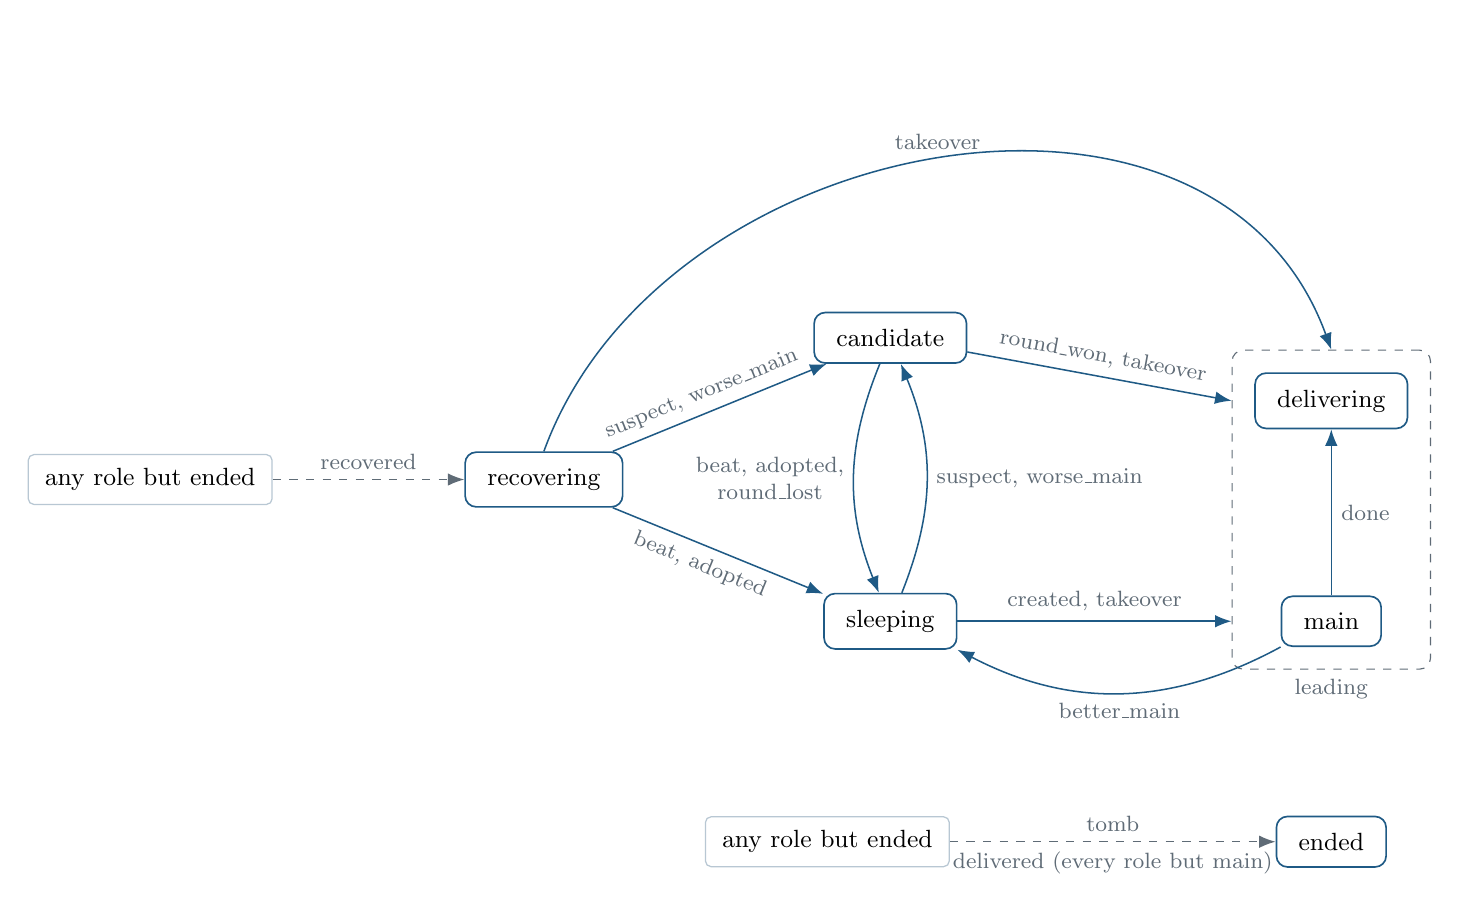
\begin{tikzpicture}
  \node[plain] (anyrec) at (-5.0,2.4) {any role but ended};
  \node[state] (rec) at (0,2.4) {recovering};
  \node[state] (cand) at (4.4,4.2) {candidate};
  \node[state] (sleep) at (4.4,0.6) {sleeping};
  \node[state] (deliv) at (10.0,3.4) {delivering};
  \node[state] (main) at (10.0,0.6) {main};
  \node[draw=pagletsMuted,dashed,rounded corners=4pt,fit=(main)(deliv),inner sep=8pt,
        label={[event]below:leading}] (lead) {};
  \node[plain] (anyend) at (3.6,-2.2) {any role but ended};
  \node[state] (ended) at (10.0,-2.2) {ended};

  \draw[dashedarrow] (anyrec) -- node[event,above] {recovered} (rec);
  \draw[arrow] (rec) -- node[event,above,sloped,pos=0.45] {suspect, worse\_main} (cand);
  \draw[arrow] (rec) -- node[event,below,sloped,pos=0.45] {beat, adopted} (sleep);
  \draw[arrow] (sleep) to[bend right=22] node[event,right] {suspect, worse\_main} (cand);
  \draw[arrow] (cand) to[bend right=22] node[event,left,align=center] {beat, adopted,\\round\_lost} (sleep);
  \draw[arrow] (cand) -- node[event,above,sloped] {round\_won, takeover} (lead.west |- deliv);
  \draw[arrow] (sleep) -- node[event,above] {created, takeover} (lead.west |- main);
  \draw[arrow] (main.south west) to[bend left=28] node[event,below] {better\_main} (sleep.south east);
  \draw[arrow] (rec.north) to[out=70,in=110,looseness=1.1] node[event,above] {takeover} (lead.north);
  \draw[arrow] (main) -- node[event,right] {done} (deliv);
  \draw[dashedarrow] (anyend) -- node[event,above] {tomb} node[event,below] {delivered (every role but main)} (ended);
\end{tikzpicture}}
\caption{The roles and the transitions of Listing~\ref{lst:zombie-transitions}. An arrow carries the causes of the change. An arrow into the dashed box ends in \code{main}, or in \code{delivering} when the checkpoint taken over is already final. \code{recovered} leads from every role but \code{ended} to \code{recovering}; \code{tomb} leads from every role but \code{ended} to \code{ended}, \code{delivered} from every role but \code{main} and \code{ended}.}
\label{fig:zombie-roles}
\end{figure}

\subsection{Beats, elections and takeovers}\label{sec:zombies-takeover}

Replicas exchange seven messages (Table~\ref{tab:zombie-messages}). Every
message carries a term, and a receiver raises its own highest term to it.
Four timers drive the rest: \code{beat}, \code{checkpoint}, \code{suspect}
(a sleeping or recovering replica has heard no beat for a while) and
\code{round} (an election round ends; a main's pause ends).

\begin{table}[htbp]
\centering\small
\caption{The messages of the protocol (\code{zombie.hpp}).}
\label{tab:zombie-messages}
\begin{tabular}{lp{4.3cm}p{7.6cm}}
\toprule
Message & From, to & Content \\
\midrule
\code{beat} & main to every member & rank of its checkpoint, version vector of its journal, its membership \\
\code{ack} & replica to the main whose beat it heard & its rank and version vector, when it lacks something \\
\code{checkpoint} & main to one replica & the work (if the replica is behind) and the entries it lacks \\
\code{entries} & replica to main & entries the main lacks \\
\code{status?} & candidate to every member & asks for role and rank \\
\code{status} & the answer & role, rank, highest term seen \\
\code{takeover} & candidate to the best replica of its round & take over as main \\
\bottomrule
\end{tabular}
\end{table}

\textbf{Suspicion and election.} A sleeping replica that hears no beat for
\code{suspect\_ms} (10\,s) plus a random jitter of up to \code{jitter\_ms}
(5\,s) becomes a candidate and broadcasts \code{status?}. When its round
ends after \code{round\_ms} (4\,s), it picks the best of itself and every
replica that answered: the higher rank; among equal ranks a replica that
already leads; then the lower replica ID. If it is best itself, it becomes
main with a new reign. Otherwise it sends \code{takeover} to the best
replica, unless that one leads already, and follows it (\code{decide()}).
A candidate that hears a beat of a main at least as far as itself goes
back to sleep at once. A main that is asked for its status checkpoints
first and pauses its work for one round, so the rank it reported stays
true while the round is open.

\textbf{Two mains meet.} When a partition heals, each main hears the
other's beat. The one behind steps down at once: it stops its work, becomes
sleeping, acknowledges the other's checkpoint and hands over the journal
entries the other lacks. The one ahead answers with its own beat and pauses
for a round, so its rank stays what the other compares with
(\code{meet()} in \code{zombie\_impl.hpp}). The conflict is settled in at
most two exchanges, even while both keep working. Because the order on
ranks is total, two mains that meet always agree on the same one. That any
number of mains converge to one, whatever the order of meetings, is the
goal \code{one\_main} of Section~\ref{sec:zombies-model}: checked in full
for two replicas, and for three replicas only by the timed runs.

\textbf{Restarts.} After its host restarts, a replica comes back from its
memory image as \code{recovering}, whatever it was, with a new incarnation
and the working state beyond its checkpoint dropped. It listens for the
suspect timeout before it may run for election. A former main does not
resume on its own; if nobody is further along, it wins the election with
its checkpoint. After a shutdown of the whole mesh, the group is down until
hosts come back; then the most advanced replica among them continues.

\textbf{Membership growth.} The membership is a set of replica IDs that
only grows. Beats carry it, and a message from a replica not in the set
adds the sender. Every \code{expand\_ms} (30\,s) the acting main asks
\code{mesh-info} for the hosts of the mesh, clones itself to every host
that offers the \code{zombies} service and holds no replica of the group,
and adds the new replicas (input \code{AddMembers}); a host that joins the
mesh later is occupied this way within about a minute. If the mains of two
sides of a partition both make a replica on the same new host, that host's
registry refuses the second one, which ends. A host that leaves stays a
member; messages to it are lost.

\subsection{Journals and checkpoints}\label{sec:zombies-journals}

The state of a zombie has two parts. The \emph{work} is the job's state:
the winning lineage keeps its work, the others drop theirs. The
\emph{journal} holds the observations the \paglet{} made with
\code{observe()}; it is merged, never dropped. An entry is keyed by the
observing replica, its incarnation (raised on every restart, so numbers are
never reused) and a number counting from~1. Journals merge by union, which
is commutative, associative and idempotent: replicas that exchanged their
entries hold the same journal, whatever the order of exchanges. A
\emph{version vector}~\cite{parker1983versionVectors} summarizes a journal
by the gap-free prefix it holds
per observer and incarnation. A beat carries the main's version vector; a
replica that hears it asks for what it lacks (\code{ack}, answered with a
\code{checkpoint} message) and hands over what the main lacks
(\code{entries}).

A checkpoint is the main's working state and its journal, recorded with a
new rank. The main makes one, if anything changed since the last, when
the \code{checkpoint} timer fires (\code{checkpoint\_ms}, 10\,s), when it
is asked for its status and when it meets another main; and always when
the work is done. A
sleeping replica that receives a checkpoint message further along than its
own replaces its work with it; the entries are merged in any case. One rule
binds every environment that runs the state machine: \emph{durable before
visible}. The outputs of a step are carried out in order, and a
\code{Persist} output completes, the replica's state being durable, before
any later output of the same step takes effect. A main's checkpoint is
therefore stored before any replica hears of it, and a replica that adopts
a checkpoint or merges entries stores them before it answers. Not
everything a beat says is durable yet: its version vector names the
observations the main made since its last checkpoint, and its membership
the hosts it occupied since; both become durable with the main's next
checkpoint, or on a replica that asks for the entries.

\subsection{Exactly one result: the sink}\label{sec:zombies-sink}

The sink of a group is \code{host:NAME}, a host of the mesh by its ledger
name or its key ID (or a prefix of it of at least 8 hex digits). Its
\code{zombies} system \paglet{} (Section~\ref{sec:mesh}) accepts the first
result per group and sink number, stores it on that host before it
answers, and answers every later delivery with \code{accepted: false}.
Results are limited to 4\,MB: a larger one is refused by the delivering
host's own \code{zombies} service with the error \code{quota}, which the
SDK treats like an unreachable sink, so the main tries again with every
beat and the group does not end until the owner cancels it (a limit of the
current implementation). Whatever the sink answers, the group is done: the
delivering main outputs a \code{Tombstone} and ends with cause
\code{delivered}. Its host records the tombstone, and every host sends
what it knows about ended and redirected groups to every other host every
5\,s, and a new tombstone or redirect at once, so the tombstone reaches every host,
also one that was offline and comes back later; a replica learns of it from
its own host (input \code{RegistryUpdate}) and ends with cause \code{tomb}.
Tombstones are kept for 30 days. During a partition both sides may finish
and deliver; the sink accepts one, the other main learns \emph{already
delivered} and ends too.

The owner can end a group at any time (\code{paglets-host remote zombies
cancel GROUP}), which writes a tombstone of its own. If the sink cannot
come back, the owner can \emph{redirect} the group to another host, which
raises the group's \emph{sink number}. Sink numbers spread like tombstones,
every replica keeps the highest it has seen, and a delivering main delivers
to the highest it knows. A redirect is the owner's statement that the old
sink accepted nothing; if it had, two sinks hold a result. The checked
property is therefore \emph{at most one result, plus one for every
redirect}.

\subsection{The state machine and the SDK}\label{sec:zombies-sdk}

The specification is the transition function \code{Outputs step(State\&,
const Input\&)}: it applies one input to a replica and returns what the
environment must do, in order. An \code{Input} is a timer that fired, a
message that arrived,
the \paglet{}'s work (\code{Worked}, \code{Observed}), the sink's answer, a
change of the host's registry, new members, the start of the group, or a
restart (\code{Recovered}). An \code{Output} is a message to send,
\code{Persist}, a timer to set or stop, \code{StartWork} and
\code{StopWork}, \code{Deliver}, \code{Tombstone}, \code{End}, or a
\code{Transition} record. \code{State} and the messages have MessagePack
encodings.

The guest SDK runs this function in the class template
\code{paglets::patterns::Zombie<Work>}, header \code{patterns/zombie.hpp}
of the SDK. A \paglet{} derives from it and provides three things:
\code{step(work, finished)}, one step of the work on the acting main, which
calls \code{finished(done)} once, also after waiting for replies;
\code{progress(work)}, a number that only grows; and \code{result(work,
journal)}, the bytes for the sink. It may override \code{result\_name()}
(default \code{result.bin}), \code{on\_role()}, which reports every role
change, and \code{on\_zombie\_failed()}. \code{Work} is any type with \code{paglets\_encode} and \code{paglets\_decode}, for
example one from a schema header. The creator calls
\code{start\_group(sink, work, timing)}, typically from a request handler;
it starts as the main, asks \code{mesh-info} for the hosts, which must all
offer \code{zombies}, and clones itself to every other host. The Mesh
Chronicle's step asks \code{mesh-info} for the landscape and records what
changed (Listing~\ref{lst:chronicle-step}); \code{note()}, not shown,
calls \code{observe\_value()}, which puts an entry into the journal on the
acting main only. \code{finished(false)} on a failed request means: not
done, try again after \code{step\_ms}.

% snippet: cpp/examples/chronicle/chronicle.cpp#step [float,caption={The Mesh Chronicle's step: one sample of the mesh, taken on the acting main},label={lst:chronicle-step}]
\begin{lstlisting}[style=paglets-cpp,float,caption={The Mesh Chronicle's step: one sample of the mesh, taken on the acting main \src{cpp/examples/chronicle/chronicle.cpp}},label={lst:chronicle-step}]
void step(Work& w, std::function<void(bool done)> finished) override {
    auto mi = service("mesh-info");
    if (!mi) return finished(false);
    services::mesh_info::Client client{*mi};
    services::mesh_info::LandscapeRequest q;
    q.max_age_ms = std::max<std::int64_t>(3 * w.sample_ms, 3000);
    auto sent = client.landscape(q, [this, &w, finished](Result<services::mesh_info::Landscape> r, Message&) {
        if (!r) return finished(false);
        sample(w, r->hosts);
        const bool done = finish_ || now_ms() - w.started_ms >= w.lifetime_ms;
        if (done) note(Event{now_ms(), "end", here_, {}, std::to_string(w.samples) + " samples"});
        finished(done);
    });
    if (!sent) finished(false);
}
\end{lstlisting}
% /snippet

A step may wait, and the main may stop meanwhile: it met a main further
along, or a candidate's round paused it. The base class fences the step
with a generation, so a late \code{finished} of a stopped main is ignored:

% snippet: cpp/sdk/include/paglets/patterns/zombie.hpp#run_step
\begin{lstlisting}[style=paglets-cpp]
void run_step(std::uint64_t gen) {
    step(work_, [this, gen](bool done) {
        if (gen != work_gen_ || !acting()) return;  // stopped meanwhile: the result is void
        run(zp::Worked{progress(work_), done, encode(work_)});
        if (!done && gen == work_gen_ && acting()) schedule_step();
    });
}
\end{lstlisting}
% /snippet

\noindent The base class carries out the outputs. Messages go to the other
replicas through endpoints from the host's \code{zombies} registry (every
host tells the others which replica of a group it holds; apart from the
endpoint to its creator that a clone receives, no capability is passed
between replicas, and after a restart the endpoints are asked from the
registry again); timers are \code{after()} messages
to itself, fenced by a generation too; a \code{Transition} is recorded as a
trace on the host and reported through \code{on\_role()}. \code{Persist}
is where ABI v1.2 (Section~\ref{sec:lifecycle}, Appendix~\ref{app:abi})
comes in: \code{checkpoint()} stores the \paglet{}'s memory image right
after the current handler, before its next message. The base class calls it
for a \code{Persist} output and defers the remaining outputs of that step to
its next handler, which it reaches by an asynchronous message to itself
(Listing~\ref{lst:zombie-carry-out}). This is how \emph{durable before
visible} is kept in the guest.

% snippet: cpp/sdk/include/paglets/patterns/zombie.hpp#carry_out [float,caption={Durable before visible in the SDK: after a \code{Persist}, the rest of a step waits for the next handler, when the image is stored},label={lst:zombie-carry-out}]
\begin{lstlisting}[style=paglets-cpp,float,caption={Durable before visible in the SDK: after a \code{Persist}, the rest of a step waits for the next handler, when the image is stored \src{cpp/sdk/include/paglets/patterns/zombie.hpp}},label={lst:zombie-carry-out}]
// Carries out the outputs from `i` on. After a Persist the rest waits
// for the next handler, when the image is stored.
void carry_out(const zp::Outputs& outs, std::size_t i) {
    for (; i < outs.size(); ++i) {
        const auto& o = outs[i];
        if (std::holds_alternative<zp::Persist>(o)) {
            (void)checkpoint();
            deferred_.insert(deferred_.end(), outs.begin() + static_cast<std::ptrdiff_t>(i) + 1, outs.end());
            if (!flush_pending_) {
                flush_pending_ = true;
                SendOptions options;
                options.async = true;
                (void)self().send("zombie.flush", std::move(options));
            }
            return;
        }
        if (!deferred_.empty()) {  // keep the order behind earlier deferred outputs
            deferred_.push_back(o);
            continue;
        }
        apply(o);
    }
}
\end{lstlisting}
% /snippet

The base class calls \code{set\_restart(true, true)}
(Section~\ref{sec:lifecycle}) when the group starts and when a clone
arrives, so that a replica comes back from its last image after a host
restart and receives \code{on\_recovered} first. The base class answers it
with the \code{Recovered} input, drops the deferred outputs and
timers of before the restart, asks the registry for endpoints and for what
it learnt meanwhile, and the replica comes back as \code{recovering}.

\subsection{Checking the protocol}\label{sec:zombies-check}

The protocol is checked in three ways: two run the transition function,
the third checks live traces against its transition table and rank order.
The first two are run by \code{paglets-protocol-check}
(\path{cpp/tools/protocol_check}); the third runs on live meshes.

\subsubsection{The model checker}\label{sec:zombies-model}

\code{paglets::verify} (\code{verify/explorer.hpp} next to the protocol)
is an explicit-state model checker for protocols written as pure transition
functions. A model gives it a finite world: the initial state, the
successors of a state, each labelled and marked as a fault or not, a
canonical encoding, invariants and goals. \code{explore()} visits every
reachable state breadth-first, one level at a time on all hardware threads,
and checks the invariants on every state; a violation comes with the
shortest sequence of steps that leads to it. Goals are checked on the graph
of fault-free steps by backward reachability from the goal states: from
every reachable state, a goal state must be reachable without further
faults. In the terms of temporal logic this is $\mathrm{AG}\,\mathrm{EF}\,
\mathit{goal}$, with AG over every reachable state and EF over fault-free
steps only; for a single goal state it is the home-state property of
Petri-net analysis~\cite{murata1989petri}, for a set of goal states its
generalization to a home space: no dead end and no trap, so that whatever the faults did, once
they stop, the goal stays reachable, and any scheduler that takes every
enabled step with positive probability reaches it with probability~1. It is
not a liveness proof under fairness; that is future work (below).

The zombie model (\code{protocols/zombie/model.hpp}) is a few hosts, each
with one replica, its durable state and its registry entry (tombstone, sink
number); the sinks; the links; and the messages in flight, in one ordered
channel per sender and receiver, as the transport keeps one queue per peer.
Faults are steps like any other, limited by a budget per world: a host
crashes (losing what was not durable, and the messages to it); a link is
cut; a message is lost or delivered twice; a sink goes down; the owner
cancels or redirects; a timeout fires early, that is, while what it detects
is not true. Timers may fire at any time otherwise, so safety does not
depend on timing. Restarting, healing, gossip, delivery and the work are
not faults. The job in these worlds is one progress step and one
observation. Four invariants and two goals are checked
(Table~\ref{tab:zombie-properties}); Listing~\ref{lst:zombie-property}
shows one invariant.

\begin{table}[htbp]
\centering\small
\caption{The properties of the zombie model (\code{model.hpp}).}
\label{tab:zombie-properties}
\begin{tabular}{llp{8.6cm}}
\toprule
Property & Kind & Meaning \\
\midrule
\code{one\_result} & invariant & at most one sink holds a result, one more for every redirect \\
\code{best\_progress\_kept} & invariant & while the group lives, some replica durably holds the best checkpoint that was ever durable \\
\code{observations\_kept} & invariant & while the group lives, every observation that was ever durable is durable on some replica \\
\code{legal\_transitions} & invariant & every role change is in the table \\
\code{one\_main} & goal & a single main, followed by every other replica with its checkpoint, journal and membership (or the group ends) \\
\code{group\_ends} & goal & every replica ended, after a sink accepted the result (or the owner cancelled) \\
\bottomrule
\end{tabular}
\end{table}

% snippet: cpp/common/include/paglets/protocols/zombie/model.hpp#invariant [float,caption={An invariant of the model: the best durable checkpoint is never lost. \code{w.best} is a ghost variable, the best rank that was ever durable on any host},label={lst:zombie-property}]
\begin{lstlisting}[style=paglets-cpp,float,caption={An invariant of the model: the best durable checkpoint is never lost. \code{w.best} is a ghost variable, the best rank that was ever durable on any host \src{cpp/common/include/paglets/protocols/zombie/model.hpp}},label={lst:zombie-property}]
{"best_progress_kept",
 "while the group lives, some replica durably holds the best checkpoint ever made durable",
 [](const State& w) {
     if (tombed(w)) return true;
     for (const auto& h : w.hosts) {
         if (h.durable.role != Role::ended && h.durable.rank >= w.best) return true;
     }
     return false;
 }},
\end{lstlisting}
% /snippet

The canonical encoding keeps the state space finite. Terms are only
compared, raised to a maximum and incremented, so the encoding renames
them: the terms that occur anywhere in a world are mapped in order onto
small numbers, with gaps shrunk to~2 (\code{canonicalize()} in
\code{model.hpp}), and two worlds that differ only in the absolute values
of their terms get the same encoding. Messages to a replica that ended are
dropped from the encoding too, since they can have no effect. Hash
compaction keeps the visited set small: states are identified by a 128-bit
hash of their encoding~\cite{stern1995hashCompaction}; the set of visited
states holds hashes, and only the states of the current level are kept as
encodings. The probability that two distinct states of a
run share a hash is about $n^2/2^{129}$ for $n$ states, below $10^{-24}$
for the largest world below; an exact mode is planned (below).

Table~\ref{tab:zombie-results} shows what was checked. Each two-replica
world is explored completely: every reachable state within its fault
budget, with all six properties. The three-replica worlds are explored to a
depth of 11 steps from the initial state (with at most two messages in
flight per channel): the invariants hold on every state within that depth,
and the goals are not checked there, because backward reachability needs
the complete graph. Across the full suite, every entry of the transition
table occurs.

% hand-copied from docs/results/zombie_protocol.json (recorded 2026-10-13):
% the `% results: zombie_protocol` marker renders one float holding a wide
% table and thirteen per-test tables, which is too large for a page; see the
% refinement plan. Replace this table with the marker once paglets-docs-sync
% has a compact layout for LaTeX results tables. Until then keep these
% numbers in step with the JSON (checked 2026-10-14).
\begin{table}[htbp]
\centering\small
\caption{Model checking of the zombie protocol: the exhaustive worlds of the full suite, as recorded on 2026-10-13 (Darwin arm64, Release build). Every world has two replicas unless stated, a job of one step and one observation, and at most three messages in flight per channel (three replicas: two). Every named fault may occur once (two crashes: twice). Depth is the longest shortest path from the initial state, or the bound of a bounded exploration. The suite is \code{paglets-protocol-check --suite full}; the numbers are those of \code{docs/results/zombie\_protocol.json}.}
\label{tab:zombie-results}
\begin{tabular}{lrrrr}
\toprule
World & States & Steps & Depth & Time (s) \\
\midrule
crash, cut & 12\,908\,826 & 50\,102\,693 & 47 & 565.9 \\
crash, loss & 3\,961\,354 & 17\,259\,715 & 43 & 182.8 \\
crash, duplicate & 4\,380\,410 & 18\,416\,904 & 40 & 205.8 \\
crash, early timeout & 7\,807\,220 & 30\,116\,664 & 47 & 308.0 \\
two crashes & 22\,356\,397 & 81\,063\,681 & 53 & 519.2 \\
cut, loss, early timeout & 4\,000\,767 & 19\,983\,567 & 41 & 85.1 \\
crash, cancel & 3\,935\,759 & 19\,606\,519 & 41 & 54.9 \\
sink down, redirect & 378\,252 & 1\,698\,056 & 30 & 5.0 \\
one joining later: crash, cut & 13\,205\,168 & 51\,296\,859 & 49 & 215.5 \\
one joining later: crash, early timeout & 8\,051\,595 & 31\,115\,057 & 49 & 102.6 \\
\midrule
three replicas: crash, cut (bounded) & 9\,188\,336 & 24\,420\,885 & 11 & 79.3 \\
three replicas: two crashes (bounded) & 5\,461\,027 & 14\,745\,614 & 11 & 40.7 \\
\bottomrule
\end{tabular}
\end{table}

\subsubsection{Timed runs}\label{sec:zombies-sim}

The exhaustive check abstracts time away. A simulator
(\code{protocols/zombie/sim.hpp}) adds it back: the same \code{step()}
under virtual clocks, with the real timer durations, message latency of
1--50\,ms, a worker that makes one progress step per second for 300 steps
and an observation every ten, and random faults: crashes with a restart
after 5--60\,s, cuts healed after 5--90\,s, 2\% loss and 1\% duplication,
during a fault phase of 180\,s with a mean of 15\,s between faults. Three
replicas take part, one on a host that joins during the run. Each run has
a sink that, like the real one, accepts the first result and refuses later
ones; the run checks that a result was delivered, that every replica ends,
that the delivered journal holds every observation that was durable anywhere at
delivery, that every role change is in the table, and that a takeover
after the main crashed, with nothing else happening until a main worked
again, took at most $\mathit{suspect} + \mathit{jitter} + 2\,\mathit{round}
+ \mathit{beat} + 4\,\mathit{latency}_{\max}$, which is 25.2\,s with the
defaults. Every run is reproducible from its seed (\code{--trace SEED}
prints its role changes and faults). The 10\,000 runs recorded with
Table~\ref{tab:zombie-results} contain 119\,289 faults and 3\,370 measured
takeovers, the longest of 18.9\,s, and no failure. These runs sample
instead of enumerating, and they check a different, partly weaker, set of
properties than the model; they are an addition, not the proof.

\subsubsection{Live conformance}\label{sec:zombies-traces}

Replicas record their protocol steps on their hosts through the
\code{zombies} service: every role change with its cause and the replica's
rank, and every answer of a sink. \code{paglets-host remote zombies check
GROUP} collects these records from every live host and checks them against
the specification (\code{protocols/zombie/trace.hpp}): every role change is
in the table, no replica's rank falls except across a restart, nothing is
recorded after a replica ended, and at most one result was accepted, one
more for every redirect. This check connects the live system to the model,
and it marks what the model leaves out. The model carries the protocol's
messages but not the transport that moves them; it reduces the hosts'
gossip to a merge of tombstone and sink number between two live hosts, the
\code{zombies} service to a registry entry per host and an atomic register
per sink, and the SDK's carrying out of outputs (timers, endpoints, clones
to new hosts, the memory image) to steps of its own. The trace check, in
turn, sees only role changes, ranks and sink answers, not the messages. The
in-process tests and the live run of the Mesh Chronicle
(Section~\ref{sec:evaluation}) end with this check, and passed it.

\subsubsection{What is verified, and what is not}\label{sec:zombies-claims}

To state it precisely: in every two-replica world of
Table~\ref{tab:zombie-results}, the four invariants of
Table~\ref{tab:zombie-properties} hold in every reachable state, and from
every reachable state each of the two goals is reachable over fault-free
steps, under the fault budgets of those worlds (for example one crash and one cut, or two
crashes), a job of one step and one observation, at most three messages in
flight per channel, and up to the hash compaction's omission probability.
The four invariants hold in every state within 11 steps of the three-replica
worlds. Longer jobs, more faults and three or more replicas over their
whole state space are covered only by the timed runs and the live checks.
The model has limits of its own: it reduces the registry's gossip to a
merge step between two live hosts, and it treats a sink as a single atomic
register.

Several tightenings are planned so that these claims become sharp. An
exact mode of the checker without hash compaction for the two-replica
worlds, so that those results are exact and the omission probability is
quoted only for larger worlds. A fair-cycle check (every bottom strongly
connected component of the fault-free graph contains a goal state), which
gives liveness under weak fairness next to the recoverability result. A
mutation suite: known bugs seeded into the protocol (a dropped hand-over,
a stale beat accepted, the sink number skipped on a redirect), each shown
to be caught with a counterexample. A written soundness argument for the
term renaming, with an assertion in the model that a transition never does
more with a term than compare, maximize and increment. And three replicas
in full, by partial-order reduction or disk-backed state storage, or a
cutoff argument that $n$ replicas behave like two or three.

\section{Evaluation}\label{sec:evaluation}
% Copyright (c) 2026 by C. Klukas.
% Licensed under the MIT License. See LICENSE for details.

We evaluate four questions: can an instance resume on a different kind
of host; what does migration cost and how much does page reuse save;
how do AOT jobs change computation time; and which replication properties
do the checks establish? Appendix~\ref{app:reproduce} links raw records,
build configurations and scripts. Each experiment retains its original
build information; measurements from different builds are not combined
into one performance claim.

\subsection{Setup and measurement scope}\label{sec:evaluation-setup}

The performance tests use three machines on one local area network (LAN):
a Mac Studio (Mac13,1, arm64, 10 CPUs), a Raspberry Pi~4 and a uConsole
with Compute Module~5 (CM5; both Linux arm64, four CPUs). For the
2026-10-15 movement tests, the Mac used GCC~16.2 RelWithDebInfo with
hardware bounds checks; both Pis used GCC~16.1 Release with software
bounds checks. These checks prevent memory accesses outside the guest's
allowed range. Mobile instances used WAMR~2.4.5's fast interpreter in
sandboxed workers. Jobs compiled in the later tests used explicit
software bounds checks on all three hosts. These configuration differences
mean that timing differences cannot be attributed to CPU hardware alone.

Durations use local monotonic clocks, which do not jump with changes
to system time. We never calculate an interval by subtracting timestamps
from different hosts. The source's measurement ends when it receives the
arrival-hook acknowledgement, including the return network trip.
Individual phase medians do not sum to this total: phases can overlap,
and destination activation includes fetching the module and selecting a
worker as well as restoring state. The move table gives ten samples per
row, with median phase times and the minimum and maximum acknowledgement
times. The ranges describe observed samples; they are not confidence
intervals.

\subsection{Portability and state representation}\label{sec:evaluation-images}

The counter snapshot test restores a 131\,212-byte image (about 128\,KB):
two 64\,KB pages plus 140 bytes for metadata and the mutable global.
The restored instance returns the expected accumulated count while the
original continues independently. This checks a C++ object containing
pointers without custom state-serialization code. It does not test every
guest compiler or WebAssembly extension.

The current performance tests move between macOS and Linux, but both
ends use arm64 CPUs. Evidence for moves between CPU architectures comes
from the earlier M0 milestone, using ABI version~0: one counter module
resumed in four transfers involving macOS arm64, Linux arm64 and macOS
x86-64 under Rosetta~2. This supports the image representation used at
that milestone; it is not a current performance test on native x86.
Later correctness tests added a physical Windows~11 x86-64 host. Those
basic functional tests are not Windows performance measurements.

Separate long-operation regressions on macOS exercised scan progress,
cancellation and authority checks, and a scan with injected filesystem
latency lasting over two minutes while status requests remained responsive.
Memory tests grew a job's linear memory to a declared 2\,GB allowance;
duration tests checked admission of unknown, unlimited and week-long
budgets. They did not run a computation for a week or reserve 2\,GB of
physical RAM. These are functional checks, not additional performance
measurements; their implementations are in
\sourcefile{cpp/tests/test_file_scans.cpp}{the scan tests} and
\sourcefile{cpp/tests/test_jobs.cpp}{the job tests}.

\subsection{Physical migration and page reuse}\label{sec:evaluation-moves}

The 2026-10-15 tests completed 480 moves across all six directed pairs
of the three machines. Each pair used 0, 1, 4 and 16\,MB of added test
data (\emph{ballast}), filled with a uniform nonzero byte value. There
were ten outbound/return pairs per size. Page caches were cleared before
each outbound trial (the \emph{cold} move); module caches remained after
first use. Each move checked state, memory size, move counters and
successful arrival. Table~\ref{tab:eval-live-move} shows Mac-to-Pi results.
The source records retain every direction and sample, phase definitions
and executable identities. In the table, ACK is the elapsed time from
capture until the source receives the arrival-hook acknowledgement.

% results: live_move [layout={compact},test-prefix={mac → pi, },strip-prefix={mac → pi, },columns={test|capture, median|destination activation/restore, median|capture to arrival-hook acknowledgement, median|capture to arrival-hook acknowledgement, minimum|capture to arrival-hook acknowledgement, maximum|pages sent, median},headers={Trial|Capture|Restore|ACK|Min|Max|Pages},widths={0.24|0.11|0.11|0.11|0.1|0.1|0.07},caption={Mac-to-Pi physical moves, ten samples per row. Times in ms: Capture, Restore and ACK are medians; Min and Max are the observed ACK range. Phase columns do not sum to ACK. Pages is the median count sent.},label={tab:eval-live-move}]
\begin{table}[htbp]
\centering\small
\caption{Mac-to-Pi physical moves, ten samples per row. Times in ms: Capture, Restore and ACK are medians; Min and Max are the observed ACK range. Phase columns do not sum to ACK. Pages is the median count sent.}
\label{tab:eval-live-move}
\setlength{\tabcolsep}{3pt}
\begin{tabular}{p{0.24\linewidth}p{0.11\linewidth}p{0.11\linewidth}p{0.11\linewidth}p{0.1\linewidth}p{0.1\linewidth}p{0.07\linewidth}}
\toprule
Trial & Capture & Restore & ACK & Min & Max & Pages \\
\midrule
0 MB ballast, cold pages & 1.98 & 7.45 & 30.75 & 21.55 & 48.1 & 2 \\
0 MB ballast, return & 1.95 & 6.93 & 26.34 & 24.06 & 31.29 & 2 \\
1 MB ballast, cold pages & 17.43 & 33.32 & 85.55 & 83.59 & 149.28 & 18 \\
1 MB ballast, return & 17.83 & 26.71 & 57.93 & 56.68 & 92.95 & 2 \\
4 MB ballast, cold pages & 65.02 & 122.02 & 297.49 & 289.65 & 362.6 & 66 \\
4 MB ballast, return & 65.18 & 100.57 & 193.28 & 186.88 & 246.28 & 2 \\
16 MB ballast, cold pages & 268.96 & 474.23 & 1181.85 & 1122.15 & 1267.97 & 258 \\
16 MB ballast, return & 257.02 & 471.33 & 845.13 & 821.93 & 905.15 & 2 \\
\bottomrule
\end{tabular}
\end{table}
% /results

For 16\,MB of ballast, cold moves sent 258 pages and return moves sent
two, reusing 256 pages. Median acknowledgement time fell from 1181.85 to
845.13\,ms. Capture still took about 260\,ms and destination activation
and restoration about 470\,ms. Reusing pages reduces network traffic,
but the source still scans and hashes memory, and the destination still
creates and restores the instance. Sending fewer bytes therefore need
not reduce move time proportionally. Uniform ballast compresses well;
these results do not measure bulk throughput for incompressible state.

Earlier LAN tests on 2026-10-12 measured mean request times of
1.16--5.16\,ms over 20 pings per directed pair and File Courier transfer
rates of 20.4--39.6\,MB/s for 16--256\,MB artifacts. These measurements
describe the network context. They neither measure migration time nor
compare mobility with remote calls for the same application. We do not
infer that moving code is faster than leaving it in place.

\subsection{Compute jobs}\label{sec:evaluation-compute}

Table~\ref{tab:eval-jobs} compares the same integer job in interpreted
and warm AOT modes on 2026-10-15, using three million iterations per
sample. Returned checksums were compared. Warm execution excludes
compilation and queueing, which were recorded separately. Dividing the
interpreter median by the AOT median gives ratios of approximately 2.3
on the Mac, 6.8 on the Pi and 6.7 on the CM5. These ratios apply to this
workload and configuration, not to arbitrary C++ code or the Pi algorithm.
There is no native-C++ baseline.

% results: live_three_host_jobs [layout={compact},columns={test|mode|samples|median elapsed|elapsed range},headers={Host|Mode|Samples|Median (ms)|Range (ms)},widths={0.12|0.3|0.1|0.13|0.2},caption={Repeated identical integer jobs. Warm AOT excludes compilation; unequal interpreter sample counts reflect repeated collection.},label={tab:eval-jobs}]
\begin{table}[htbp]
\centering\small
\caption{Repeated identical integer jobs. Warm AOT excludes compilation; unequal interpreter sample counts reflect repeated collection.}
\label{tab:eval-jobs}
\setlength{\tabcolsep}{3pt}
\begin{tabular}{p{0.12\linewidth}p{0.3\linewidth}p{0.1\linewidth}p{0.13\linewidth}p{0.2\linewidth}}
\toprule
Host & Mode & Samples & Median (ms) & Range (ms) \\
\midrule
mac & AOT job & 5 & 31.0 & 30.0 to 32.0 \\
mac & interpreter job & 10 & 72.0 & 68.0 to 82.0 \\
pi & AOT job & 5 & 27.0 & 27.0 to 29.0 \\
pi & interpreter job & 75 & 184.0 & 174.0 to 239.0 \\
uconsole & AOT job & 5 & 11.0 & 11.0 to 11.0 \\
uconsole & interpreter job & 40 & 74.0 & 68.0 to 97.0 \\
\bottomrule
\end{tabular}
\end{table}
% /results

The Pi integration test used jobs to compute 100\,000 hexadecimal digits
of $\pi$, with all three hosts contributing. It finished in 69\,s,
including one-second status polling. The decimal-output check verifies
the known first 100 digits, not the entire result. This tests the
integration of mobile coordination, jobs and artifact output, rather
than measuring a controlled AOT speedup. Windows correctness tests used
interpreted jobs only.

\subsection{Replication: model, simulation and physical test}\label{sec:evaluation-zombies}

On 2026-10-16 the checker explored ten two-replica worlds completely and
two three-replica worlds to depth~11, considering at most 11 steps from
the initial state (Table~\ref{tab:zombie-results}).
Each job has one work step and one observation. Each channel holds at
most three messages, or two in the three-replica worlds. Fault budgets
limit crashes, network cuts, message loss and duplication, early
timeouts (for example, suspecting a healthy reachable main), sink
failure, cancellation and redirection.

The model also simplifies executions. A send to an unavailable host or
full channel is lost without consuming the message-loss budget. Identical
queued resends are combined. Once the crash budget is exhausted, running
hosts' current state is treated as durable. These assumptions limit what
the checked properties imply about the deployed system.

% results: zombie_protocol [layout={compact},columns={test|reachable states|steps|longest shortest path|explored to (bounded)},headers={World|States|Transitions|Depth|Bound},test-prefix={zombie protocol, exhaustive: },strip-prefix={zombie protocol, exhaustive: |two replicas: },widths={0.42|0.16|0.16|0.07|0.07},caption={Finite-model coverage. Complete worlds check four safety invariants and two recovery goals; bounded worlds check only the four invariants. Depth counts steps on a shortest path to a state, taking the maximum over states; Bound is the search cutoff.},label={tab:zombie-results}]
\begin{table}[htbp]
\centering\small
\caption{Finite-model coverage. Complete worlds check four safety invariants and two recovery goals; bounded worlds check only the four invariants. Depth counts steps on a shortest path to a state, taking the maximum over states; Bound is the search cutoff.}
\label{tab:zombie-results}
\setlength{\tabcolsep}{3pt}
\begin{tabular}{p{0.42\linewidth}p{0.16\linewidth}p{0.16\linewidth}p{0.07\linewidth}p{0.07\linewidth}}
\toprule
World & States & Transitions & Depth & Bound \\
\midrule
three replicas: crash, cut & 9188336 & 24420885 &  & 11 \\
three replicas: two crashes & 5461027 & 14745614 &  & 11 \\
crash, cancel & 3935759 & 19606519 & 41 &  \\
crash, cut & 12908826 & 50102693 & 47 &  \\
crash, duplicate & 4380410 & 18416904 & 40 &  \\
crash, early timeout & 7807220 & 30116664 & 47 &  \\
crash, loss & 3961354 & 17259715 & 43 &  \\
cut, loss, early timeout & 4000767 & 19983567 & 41 &  \\
one joining later: crash, cut & 13205168 & 51296859 & 49 &  \\
one joining later: crash, early timeout & 8051595 & 31115057 & 49 &  \\
sink down, redirect & 378252 & 1698056 & 30 &  \\
two crashes & 22356397 & 81063681 & 53 &  \\
\bottomrule
\end{tabular}
\end{table}
% /results

Only three of the ten two-replica worlds allow an early timeout, at most
once each. In the others, the relevant failure-detection timers are
accurate. Recovery goals are not checked on searches stopped at a depth
limit. The results therefore do not prove correctness under arbitrary
timing, unbounded channels or faults, or complete three-replica
executions. The full suite also requires every declared role transition
to be reached somewhere in the tests.

A deterministic simulator adds virtual clocks, message delays and
checkpoint intervals to the same protocol function. In 10\,000 recorded
three-replica runs with random fault schedules, it selected 119\,289
crash or network-cut events and observed 3370 leadership takeovers.
Some selected events had no effect. The longest measured takeover
without a further disturbance was 18.9\,s, below the configured 25.2\,s
bound. The result-journal check covers observations saved durably on
hosts that are running when the sink accepts the result. The simulated
sink accepts once by construction; it does not independently test atomic
updates in distributed storage.

The ten-minute Mesh Chronicle test on 2026-10-13 introduced a late join,
a frozen host, restarts, a network partition and sink downtime. It
delivered a merged life log through two takeovers and one partition.
Recorded roles and ranks passed the trace checker. This is one physical
execution with a chosen failure schedule, not a measurement of general
availability or a proof that recovery always completes. The pure protocol
model omits real transport, SDK action scheduling and storage behavior.
The physical test and host regression tests cover some of these gaps.

\subsection{Test coverage and limits of the evidence}\label{sec:evaluation-tests}

The test suite exercises execution inside the host process and in
sandboxed workers. A saved full-suite run passed all 18 Mac and 17
Windows CTest entries. Later focused tests cover changed runtime, mesh,
job and example behavior on Mac, Windows, CM5 and Pi. The latest
lifecycle/checkpoint tests passed 136 matched cases across both execution
modes and all four hosts. Each run has its own version record; we do not
claim that every later revision reran every earlier test. Continuous
integration (CI) configurations for detecting memory and concurrency
errors, and decoder tests with malformed inputs, provide further
engineering checks. They do not prove that races or vulnerabilities
are absent.

The evidence is limited by the small LAN, different host configurations,
different historical builds, selected workloads and bounded fault
models. We did not compare mobile coordination with equivalent remote
calls, the Python edition or native C++. Performance tests used at most
three machines and did not exercise real NAT or relay deployments.
The results demonstrate feasibility and specific costs. Comparative
benefit and behavior at larger scales remain unestablished.

\section{Discussion and Limitations}\label{sec:discussion}
% Copyright (c) 2026 by C. Klukas.
% Licensed under the MIT License. See LICENSE for details.

The preceding sections describe what \paglets{}/cpp does. This section
says what it costs, what it does not do, and where its guarantees end.
Every limit below is stated as the code enforces it today.

\subsection{The trust model}\label{sec:discussion-trust}

A mesh has four kinds of keys: admins, owners, signers and hosts
(Section~\ref{sec:mesh}). Admins decide who belongs to the mesh and what
its policy is; owners launch \paglet{}s; signers vouch for modules; hosts
run \paglet{}s. Every decision is a signed ledger record, and the mesh
trusts the ledger, not any host. A record that needs a quorum carries the
signatures of as many admins as the quorum of its epoch demands: the
genesis record sets the two numbers, admin-set records change them, and
the separate one applies to changes of the admin set itself. A stolen
admin key is removed by the remaining admins; removals win in every
conflict, and a removed admin's later records have no effect. A mesh that
must survive a stolen admin key therefore needs an admin-set quorum of at
least two; with the default of one, a single admin can remove all others.

The sandbox protects the host from the \paglet{}; nothing protects the
\paglet{} from its host. A roaming \paglet{} reaches only the imports of
its trust class, the capabilities it holds and the quotas of
Table~\ref{tab:model-limits}; by default it runs in a worker process that
the operating system confines (\code{paglets-host} falls back to its own
process when \code{paglets-worker} is not found next to it, and
\code{-{}-in-process} and \code{-{}-no-sandbox} switch the confinement off
for debugging). The confinement differs by platform: on Linux a seccomp
filter refuses the system calls that open files, create sockets or start
programs (a deny list; an allow list is planned); on macOS a sandbox
profile denies forking, executing, networking, writing files and reading
file contents; on Windows the worker runs in a job object with a
restricted token at low integrity, without processes or writes to the
user's files, but with network access, which is not restricted yet
(\code{cpp/host/src/sandbox.cpp}). A test, \code{paglets-worker
-{}-check-sandbox}, verifies on each platform that the sandbox refuses
what it must.

A host that runs a \paglet{} holds its memory image in plain form, in the
worker and, on a host with a state directory, on disk; a compromised
enrolled host can read and change the state of every \paglet{} it runs,
speak in their names (hosts stamp the sender record of every message), and
keep the \paglet{}s it receives. It cannot issue admin records
(enrollments, policy rules, module trust, admin-set changes), because it
has no admin key; the records a host key signs are enrollment requests,
grants under an allow rule, grant releases and audit entries. It cannot
read what passes through it for other hosts, because channels are
encrypted end to end. The defenses are administrative: admins revoke the
host's enrollment, owners send \paglet{}s only to hosts with a given label
(a transfer ticket names \code{label:<label>}), and admins bind marked data
to hosts by residency rules (Section~\ref{sec:mesh}). Images are not
encrypted at rest. The mesh is, as in the Python edition
\cite{klukas2026pagletsNote}, a set of hosts one organization trusts; what
is new is that one owner's \paglet{} cannot harm another's or the host,
and that the host is told what a \paglet{} may do. By default any enrolled
owner may launch any module; \code{module-policy trusted} makes roaming
modules need module trust as well, a \code{module-trust} record that names
their signer or their hash. Neither the cryptographic protocol (Noise XX
channels, record and passport signatures) nor the sandboxes have been
reviewed outside the project.

\subsection{Images, the memory limit and growth}\label{sec:discussion-memory}

A \paglet{}'s linear memory is at most 256 pages, 16\,MB
(\code{wasm::Limits::max\_memory\_pages}). The limit is a compiled-in
default of the host, not a choice of the \paglet{}. Guests are built
without exceptions (\code{-fno-exceptions}), so there is no
\code{bad\_alloc} to catch: an allocation beyond the limit aborts, an abort
is a trap, and a trap ends the \paglet{}. Messages are at most 1\,MB and
the storage service gives 16\,MB per \paglet{}. The limits are there so
that no owner can take a host over, and they shape how a \paglet{} is
written: large data belongs in files and artifacts, which move between
hosts as capabilities of a few bytes; the \paglet{} carries the handle, not
the content. The pi example keeps only the chunks that arrive early and
writes every chunk that is next in order to a file, so that 100\,000
digits need little memory.

Images have a cost that serialization does not. WebAssembly memory grows
and never shrinks, and the allocator does not zero what it frees. A
\paglet{} that once held a 10\,MB vector keeps a 10\,MB image after the
vector is gone, because the pages are no longer zero and the image elides
only zero pages. The page manifest limits what this costs in motion: a
host that has seen the \paglet{} before receives only the pages that
changed, and a clone fanned out to a host that holds the parent's pages
sends mostly hashes, because the page cache of a host is keyed by page
hash, not by \paglet{}. Image capture hashes every non-zero page with SHA-256; in the
feasibility measurements this dominated the capture time (1\,ms for two
pages on a Mac; 6.5\,ms on a Raspberry Pi 4 that was busy with a compiler
build on all four cores at the time), and the hash is still the portable
C++ implementation in \code{cpp/host/src/sha256.cpp}.

The image is bound to its module's hash. A new version of a module cannot
take over an old image, and the runtime has no state migration between
versions: a \paglet{} that must survive a code change has to hand its
state to its successor in messages, or write it to storage. A
reflection-derived export and import of state for this case is foreseen in
the plan and not built.

What images buy is the absence of serialization code and of the bugs
that come with it: nothing is forgotten in a move, pointers inside the
heap stay valid, and the \paglet{} is any C++ object graph.
Section~\ref{sec:evaluation} gives the sizes and times of real images.

\subsection{Interpreter speed}\label{sec:discussion-speed}

\paglet{}s run in WAMR's fast interpreter. AOT and JIT are turned off in
the build (\code{PagletsWamr.cmake} in \code{cpp/cmake}): no LLVM in the
host, and no compiled code that would have to be cached per CPU
architecture. The feasibility measurements in
\code{planning/cpp-m0-results.md} put the fast interpreter at about ten
times the message throughput of the classic interpreter, a host-to-guest
call at 0.4\,\textmu{}s and a message round trip through MessagePack at
6.5\,\textmu{}s on a Mac. The live benchmark of
Section~\ref{sec:evaluation} measures about 250 million integer operations
per second on a Mac Studio and 67 million on a Raspberry Pi 4, in
\paglet{} code.

For what \paglet{}s mostly do, moving, messaging and calling services, the
interpreter is not the bottleneck: a move runs guest code only in its two
hooks, and its time goes into capturing, transferring and restoring the
image, which the benchmark test of Section~\ref{sec:evaluation-images}
measures as a whole, between two hosts in one process, and does not
split. For compute the interpreter counts: the pi example needs 313\,s for
100\,000 hexadecimal digits on three hosts. How much of this is the
interpreter was not measured: no native run of the same \code{bbp.hpp} is
recorded, and the 313\,s also contain the chunk round trips across the
mesh. A \paglet{} is the right place for the coordination of such work and
a poor place for its inner loop. The way out within the model is a system
paglet that does the heavy part outside the interpreter (the \code{ai}
gateway, for instance, hands inference to an Ollama server); AOT with a
per-architecture cache, keyed by module hash and WAMR version, is the
planned alternative and was not measured.

\subsection{What weak mobility does not solve}\label{sec:discussion-weak}

A \paglet{} moves only between handlers. There is no migration in the
middle of a computation: no stack is captured, and a handler that runs
longer than the budget of 5\,s is stopped and its \paglet{} ends. Every
long computation must therefore be sliced by its author. The pi example
converts its hexadecimal fraction into decimal digits in slices of
200\,ms, each started by a timer of zero delay, and keeps its progress in
members between the slices (Listing~\ref{lst:pi-convert}). In the listing
the loop condition \code{now\_ms() - began < 200} bounds the slice, the
members \code{limbs\_} and \code{decimal\_done\_} carry the progress, and
\code{after\_raw(0, "convert", \{\})} near the end schedules the next
slice; everything in between is the arithmetic. Between two slices the
\paglet{} can be moved, checkpointed or deactivated; inside a slice it
cannot.

% snippet: cpp/examples/pi/pi.cpp#convert [float,caption={Pi's decimal conversion, sliced into handler calls of 200\,ms},label={lst:pi-convert}]
\begin{lstlisting}[style=paglets-cpp,float,caption={Pi's decimal conversion, sliced into handler calls of 200\,ms \src{cpp/examples/pi/pi.cpp}},label={lst:pi-convert}]
// A slice of the conversion: passes of multiplying the fraction by 10^9,
// whose overflow above the point is the next nine decimal digits.
void convert() {
    if (state_ != "converting") return;
    const std::int64_t began = now_ms();
    std::string digits;
    while (decimal_done_ + static_cast<std::int64_t>(digits.size()) < decimal_total_ && now_ms() - began < 200) {
        // Only the precision the remaining digits need (and two limbs more).
        const std::int64_t remaining = decimal_total_ - decimal_done_ - static_cast<std::int64_t>(digits.size());
        const auto need = static_cast<std::size_t>(static_cast<double>(remaining) * 3.3219280949 / 32.0) + 2;
        if (limbs_.size() > need) limbs_.resize(need);
        std::uint64_t carry = 0;
        for (std::size_t i = limbs_.size(); i-- > 0;) {
            const std::uint64_t t = static_cast<std::uint64_t>(limbs_[i]) * 1'000'000'000ULL + carry;
            limbs_[i] = static_cast<std::uint32_t>(t);
            carry = t >> 32;
        }
        char nine[16];
        std::snprintf(nine, sizeof nine, "%09u", static_cast<unsigned>(carry));
        digits.append(nine, static_cast<std::size_t>(std::min<std::int64_t>(9, remaining)));
    }
    decimal_done_ += static_cast<std::int64_t>(digits.size());
    if (shown_dec_.size() < shown_digits) shown_dec_ += digits.substr(0, shown_digits - shown_dec_.size());
    if (dir_) {
        dec_file_.pending += digits;
        flush(dec_file_);
    }
    if (decimal_done_ < decimal_total_) {
        (void)paglets::after_raw(0, "convert", {});
        return;
    }
    std::vector<std::uint32_t>().swap(limbs_);
    state_ = "writing";
    maybe_done();
}
\end{lstlisting}
% /snippet

The slicing is visible in the code and is the author's responsibility; the
runtime cannot do it for a loop it does not see. Suspending a handler in
the middle (Asyncify or Wasm stack switching; WP-R1 in the plan) would
remove the slicing. It would not change what moves: a pending service
call, a timer or a reply capability lives on the host, not in linear
memory, and each follows its own rule on a move
(Section~\ref{sec:movement}) whether the handler was suspended or not.

\subsection{Platforms and editions}\label{sec:discussion-platforms}

\paglets{}/cpp is built and tested in CI on Linux x86-64 and arm64, on
macOS arm64, and under AddressSanitizer, UndefinedBehaviorSanitizer and
ThreadSanitizer. Windows is experimental: the job builds with MinGW-w64
GCC in MSYS2, runs with guest modules built by the Linux job, uses
software bound checks because MinGW cannot build WAMR's guard-page
checks, and may fail without failing the workflow
(\code{continue-on-error} in \code{.github/workflows/cpp.yml}). The
worker sandbox on Windows is the weaker one described above. On the
Raspberry Pi, kernels with a 39-bit address space hold about 60 instances
per process with guard-page checks, because each instance reserves 8\,GB
of address space. Configuring with
\code{PAGLETS\_WAMR\_HW\_BOUND\_CHECK=OFF} removes the limit (the default
is on everywhere but MinGW); software bound checks made message handling
about 2.5 times slower on macOS in the feasibility measurements.

The two editions of \paglets{} do not interoperate. They share concepts
(hosts, \paglet{}s, messages, meshes, services, compute slots) and no
format: transport, authentication, framing, movement and code differ
throughout \cite{pagletsCppDocs}. A Python host and a C++ host cannot talk
to each other, and a \paglet{} of one edition cannot run on the other.

\subsection{Three systems compared}\label{sec:discussion-comparison}

Table~\ref{tab:background-editions} placed the three systems next to
each other by what moves and how it runs;
Table~\ref{tab:discussion-editions} adds what each one pays for it. The
price of \paglets{}/cpp is the one this section
described: a fixed memory limit, an interpreter, sliced handlers, one
guest language, and a trust model that needs administration. What it buys
over the Python edition is that hosts need no application code, that a
\paglet{} cannot reach past its capabilities, and that a job survives the
loss of hosts.

\begin{table}[htbp]
\centering\small
\caption{What each system pays for an agent.}
\label{tab:discussion-editions}
\begin{tabular}{p{0.16\linewidth}p{0.23\linewidth}p{0.23\linewidth}p{0.25\linewidth}}
\toprule
 & \raggedright Aglets \cite{lange1997aglets,ferrari2004manual} & \raggedright \paglets{}, Python \cite{klukas2026pagletsNote} & \raggedright \paglets{}/cpp \tabularnewline
\midrule
\raggedright State on the wire & \raggedright the Java object, serialized; classes with it, or fetched from the codebase & \raggedright a dataclass, serialized; no code & \raggedright the non-zero 64\,KB pages the destination lacks, compressed; modules by SHA-256, fetched on demand \tabularnewline
\raggedright Memory per agent & \raggedright a share of the server's JVM heap & \raggedright a Python process per active \paglet{} & \raggedright at most 16\,MB of linear memory; an image keeps every page that was ever non-zero \tabularnewline
\raggedright Execution & \raggedright the JVM & \raggedright CPython & \raggedright a Wasm interpreter, no JIT or AOT \tabularnewline
\raggedright Long computations & \raggedright a thread per aglet & \raggedright a handler in the \paglet{}'s process; its mailbox waits & \raggedright sliced handlers; a budget of 5\,s per handler \tabularnewline
\raggedright Fault tolerance & \raggedright --- & \raggedright deactivated \paglet{}s come back from disk after a host restart; active ones are lost & \raggedright restart from the last image; zombie replicas on every host that offers \code{zombies} \tabularnewline
\raggedright Sandbox & \raggedright the Java platform & \raggedright none; a \paglet{} reaches what its process reaches & \raggedright Wasm instance, import set per trust class, sandboxed worker processes \tabularnewline
\raggedright Administration & \raggedright a Tahiti server per host & \raggedright a shared API key & \raggedright keys for every party, a signed ledger with quorums, policy, module trust, residency \tabularnewline
\raggedright Tooling & \raggedright the Tahiti server & \raggedright a CLI & \raggedright CLI, web UI, interface descriptions, protocol checker \tabularnewline
\bottomrule
\end{tabular}
\end{table}

\subsection{Open problems}\label{sec:discussion-open}

\begin{itemize}
\item \emph{Verification of the zombie protocol.} The exhaustive check is
  complete for two replicas and bounded to a depth of 11 steps for three
  (Section~\ref{sec:zombies}). Every world is explored with hash
  compaction (states identified by a 128-bit hash of their encoding,
  \code{verify/explorer.hpp}), so even the two-replica results carry a
  small omission probability, and the timed random runs sample timer
  values and takeover times instead of enumerating them. An exact mode, a
  fairness check of the fault-free graph, a mutation suite that shows the
  checker catches seeded bugs, and either a full three-replica exploration
  or a cutoff argument are planned; the repository tracks these items. The
  model also leaves out the transport, the gossip and the \code{zombies}
  service itself; the replay of recorded live traces is the conformance
  check between them.
\item \emph{Mesh size.} The live mesh has three hosts. The tests run
  meshes of four hosts in one process and a gossip test of five hosts
  under random partitions. Nothing has been measured beyond that: how the
  location records, the ledger gossip and \code{mesh-info} snapshots
  behave with tens of hosts is not known.
\item \emph{Relays and NAT.} Hosts without an inbound port take part
  through relays, and the test suite exercises this with hosts that do not
  listen, including two such hosts reaching each other and a relay going
  down (\code{cpp/tests/test\_discovery.cpp}). No live run has crossed a
  NAT or a firewall; the live hosts share one LAN.
\end{itemize}

The limits of the sections above are open as well: the security review,
state migration between module versions (foreseen in the plan, not
built), AOT compilation with a per-host cache, and the research items
WP-R1 (mid-handler migration) and WP-R2 (other guest languages: the ABI
is core WebAssembly, so a second language is a matter of an SDK, not of
the host).

\section{Conclusion}\label{sec:conclusion}
% Copyright (c) 2026 by C. Klukas.
% Licensed under the MIT License. See LICENSE for details.

This paper has made one unit of execution carry a mobile agent: a
WebAssembly module plus one instance, whose whole state is its linear
memory and its exported mutable globals. Because the host calls into the
instance one handler at a time, it takes that memory as an image between
two calls, and the image is enough to store, copy and move the \paglet{}
(Sections~\ref{sec:model} to \ref{sec:movement}). The \paglet{} writes no
serialization code; what it gives up is strong mobility, so a long
computation is sliced by its author (Section~\ref{sec:discussion-weak}).
The rest follows from this unit: lifecycle events and failure reports
are deliveries ordered with the messages (Section~\ref{sec:lifecycle}); a
move ends in location records, so endpoints keep working while their
targets move (Section~\ref{sec:communication}); hosts share a signed
ledger and nothing else, and a \paglet{} reaches resources only through
system \paglet{}s under policy (Section~\ref{sec:mesh}); a zombie
\paglet{} keeps a replica on every host and delivers exactly one result
(Section~\ref{sec:zombies}); and the interface description in the module
lets the CLI and the web client talk to any \paglet{}
(Section~\ref{sec:tools}).

The evaluation supports these claims at the scale it was tried
(Section~\ref{sec:evaluation}). The Counter's image is 131\,212 bytes, and
one module was captured and resumed across macOS arm64, Linux arm64 and
macOS x86-64 under Rosetta~2. On the live mesh of three machines, round
trips between \paglet{}s take 1.2--5.2\,ms, content moves at
20--40\,MB/s, 100\,000 hexadecimal digits of $\pi$ take 313\,s on all
three hosts, and the Mesh Chronicle delivers its log after two takeovers
and a partition with a main on both sides. Behind the numbers stand 252
test cases run in-process and with sandboxed workers, and the check of
the zombie protocol: ten two-replica worlds explored completely, two
three-replica worlds to depth 11, 10\,000 timed runs without a failure.
What the evaluation does not support is equally plain: no move between
real machines is timed, the live numbers are single runs on one LAN, no
mesh is larger than three real or five tested hosts, and nothing was
measured with AOT or JIT, through a relay, across a NAT, or on Windows.

The next steps are the ones Sections~\ref{sec:zombies-claims} and
\ref{sec:discussion-open} name. For the zombie protocol: a checker mode
without hash compaction, a fair-cycle check for liveness, a mutation
suite, a soundness argument for the term renaming, and three replicas in
full or a cutoff argument. For the mesh: tens of hosts, relays and NAT.
For the runtime: a security review, state migration between module
versions, AOT with a per-architecture cache, suspending a handler
mid-computation, and a second guest language on the same ABI.

\paglets{}/cpp is free software under the MIT License. The sources are the
branch \code{cpp} of the repository \cite{pagletsCpp}, released as
\code{cpp-v0.2.0}; on macOS the Homebrew tap \code{cklukas/homebrew-paglets}
builds the latest release (\code{brew install cklukas/paglets/paglets});
the documentation, with the examples and the recorded results, is
published at \cite{pagletsCppDocs}, and the paper's workflow puts the
PDF of every published version beside it. The excerpts and result
tables in this paper are generated from the sources and the recorded
results by the tool that keeps the documentation current
(Appendix~\ref{app:reproduce}); a test fails whenever either falls behind
the code.


\section*{Use of generative AI}\label{sec:ai}
\addcontentsline{toc}{section}{Use of generative AI}
The implementation and this paper were developed with support from
Claude (Anthropic) and Codex (OpenAI) under the author's direction.
The author is responsible for the design, technical claims and review.
Generated excerpts and tables are checked against source files and
recorded results. These checks detect text that no longer matches its
source. They do not establish that models, measurements or interpretations
are correct.

\bibliographystyle{plain}
\bibliography{references}

\clearpage
\begin{appendices}
\section{Source Files and Reproducibility}\label{app:reproduce}
% Copyright (c) 2026 by C. Klukas.
% Licensed under the MIT License. See LICENSE for details.

% This appendix is dense with monospaced option and script names that
% cannot be hyphenated; the emergency stretch keeps such paragraphs inside
% the text width (as in Appendix A).
\begingroup\setlength{\emergencystretch}{3em}

Every number in Section~\ref{sec:evaluation}, every table of recorded
results and every code excerpt whose caption names a source path is
produced by a script or a tool in the repository \cite{pagletsCpp}. This
appendix names them, in the order in which one would run them: build the
edition, run the test suite and record its results, run the live
measurements on real machines, run the protocol checker, and regenerate the
documentation and this paper from the recorded results.
Figure~\ref{fig:reproduce-pipeline} shows how the pieces connect. The
commands below run from the repository root of the branch \code{cpp}; those
that concern this paper (Section~\ref{sec:reproduce-generated}) need the
branch \code{cpp-paper}, which carries \code{papers/} and takes \code{cpp}
in by merge. The page \code{building.md} of the user documentation
\cite{pagletsCppDocs} describes the build and the test suite in more
detail; \code{examples/index.md} (``Test results'') says how the examples'
results are recorded.

\begin{figure}[htbp]
\centering
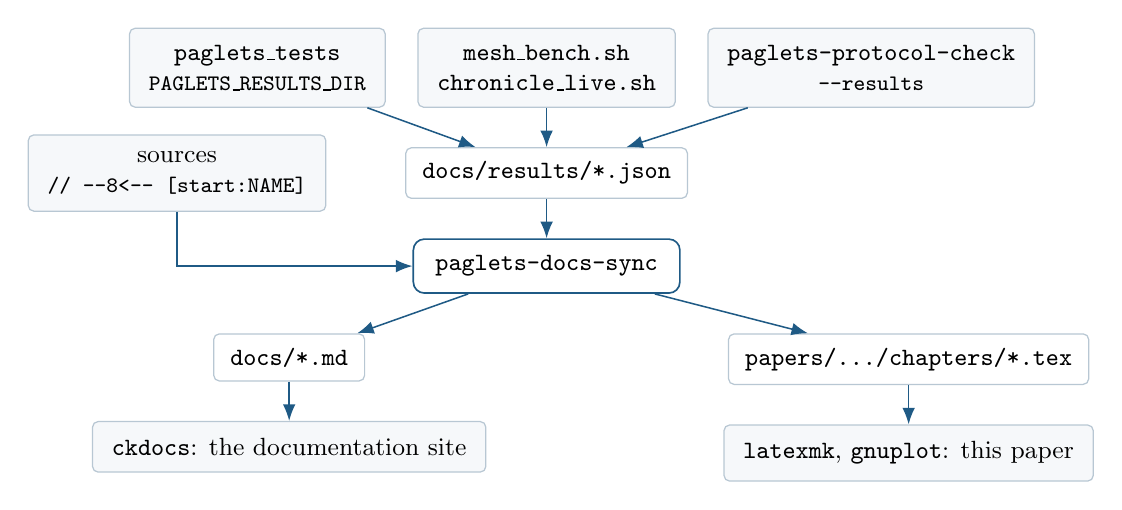
\begin{tikzpicture}[node distance=5mm and 4mm]
  \node[box] (tests) {\code{paglets\_tests}\\\footnotesize\code{PAGLETS\_RESULTS\_DIR}};
  \node[box, right=of tests] (live) {\code{mesh\_bench.sh}\\\code{chronicle\_live.sh}};
  \node[box, right=of live] (check) {\code{paglets-protocol-check}\\\footnotesize\code{-{}-results}};
  \node[plain, below=of live] (json) {\code{docs/results/*.json}};
  \node[box, left=of json, xshift=-6mm] (src) {sources\\\footnotesize\code{// -{}-8<-{}- [start:NAME]}};
  \node[state, below=of json] (sync) {\code{paglets-docs-sync}};
  \node[plain, below left=of sync, xshift=-2mm] (md) {\code{docs/*.md}};
  \node[plain, below right=of sync, xshift=2mm] (tex) {\code{papers/.../chapters/*.tex}};
  \node[box, below=of md] (site) {\code{ckdocs}: the documentation site};
  \node[box, below=of tex] (pdf) {\code{latexmk}, \code{gnuplot}: this paper};
  \draw[arrow] (tests) -- (json);
  \draw[arrow] (live) -- (json);
  \draw[arrow] (check) -- (json);
  \draw[arrow] (json) -- (sync);
  \draw[arrow] (src) |- (sync);
  \draw[arrow] (sync) -- (md);
  \draw[arrow] (sync) -- (tex);
  \draw[arrow] (md) -- (site);
  \draw[arrow] (tex) -- (pdf);
\end{tikzpicture}
\caption{Where the numbers and the excerpts come from. Tests, live scripts
and the protocol checker record results as JSON; \code{paglets-docs-sync}
writes tables from them, and code excerpts from marked regions of the
sources, into the documentation pages and into the chapters of this paper.}
\label{fig:reproduce-pipeline}
\end{figure}

\subsection{Building}
\label{sec:reproduce-building}

The host is C++26 code built with GCC~16 (\code{-std=c++26 -freflection});
reflection generates the wire codecs and the guest schema code. Guest
modules are compiled by clang for \code{wasm32-wasip1} with a WASI sysroot.
The build fetches WAMR and cpp-httplib at pinned releases. On macOS the
toolchain comes from Homebrew, on Linux GCC~16 is combined with the
wasi-sdk in \code{/opt/wasi-sdk} (or \code{WASI\_SDK\_PATH}):

\begin{lstlisting}[style=paglets-bash]
# macOS
brew install gcc@16 llvm lld wasi-libc wasi-runtimes cmake ninja \
    libsodium openssl@3 zstd pkgconf
# Linux
apt install libsodium-dev libssl-dev libzstd-dev pkg-config
\end{lstlisting}

The build and the tests use CMake presets (Table~\ref{tab:reproduce-presets}).
The presets configure \code{RelWithDebInfo} builds; the results recorded in
\code{docs/results/} come from Release builds (configured with
\code{CMAKE\_BUILD\_TYPE} set to \code{Release}), as their \code{build}
field says:

\begin{lstlisting}[style=paglets-bash]
cd cpp
cmake --preset macos-arm64
cmake --build --preset macos-arm64
ctest --preset macos-arm64
build/macos-arm64/host/paglets-host --info
\end{lstlisting}

\code{paglets-host -{}-info} prints what a build contains: version,
platform, compiler, whether reflection is on, the WAMR release with its
interpreter and bound-check mode (for example \code{fast-interp, hardware
bound checks}), the paglet ABI and the mesh protocol. The build directory
is \code{cpp/build/<preset>}; the guest modules end up in its
\code{guests/} directory. Two configure options matter for the
measurements. \code{PAGLETS\_WAMR\_FAST\_INTERP}, on by default, selects
WAMR's fast interpreter. \code{PAGLETS\_WAMR\_HW\_BOUND\_CHECK} must be
off on kernels with a 39-bit address space such as Raspberry Pi OS, where
guard-page bound checks limit a process to about 60 instances. A Linux
host of this kind (a GCC~16 installed next to an older system compiler, as
on Raspberry Pi OS) is built with the recipe in \code{docs/building.md}
(``Build and test''): a Release build of \code{paglets-host} and
\code{paglets-worker} only, guests and tests off, hardware bound checks
off, the C++ library linked statically. Such a host needs no guest modules
of its own; the modules travel from the machine that launches the paglets.
The recorded runs describe the hosts only as
Table~\ref{tab:eval-hosts} shows them; how each host was built is
not recorded.

\begin{table}[htbp]
\centering\small
\caption{The CMake presets (\code{cpp/CMakePresets.json}).}
\label{tab:reproduce-presets}
\begin{tabular}{ll}
\toprule
Preset & Use \\
\midrule
\code{macos-arm64}, \code{linux-gcc16} & the regular builds \\
\code{windows-mingw-gcc16} & the regular build with MinGW-w64 (MSYS2 UCRT64) \\
\code{macos-arm64-asan}, \code{linux-gcc16-asan} & AddressSanitizer, UndefinedBehaviorSanitizer \\
\code{linux-gcc16-tsan} & ThreadSanitizer \\
\code{linux-host-only} & a C++23 compiler without reflection; prebuilt guests \\
\bottomrule
\end{tabular}
\end{table}

\subsection{The test suite and the recorded results}
\label{sec:reproduce-tests}

\code{ctest} runs \code{paglets\_tests} twice, with \paglet{}s inside the
test process (\code{unit}) and in sandboxed worker processes
(\code{unit\_workers}), and a dozen tests of the programs: the sandbox
check, memory images saved and resumed across processes, hosts that serve,
move and find each other, the CLI ledger, and the installed package
(\code{docs/building.md}, ``The test suite''). The \code{unit} test also
explores six small worlds of the zombie protocol exhaustively and runs 200
timed random runs (\code{cpp/tests/test\_protocol\_check.cpp}). A further
test, \code{docs\_sync}, fails while a documentation page or a chapter of
this paper is not current (Section~\ref{sec:reproduce-generated}).

The tests of the example paglets record what they measure. With
\code{PAGLETS\_RESULTS\_DIR} set, a test that reports to a topic is written to
\code{<dir>/<topic>.json} after it ran: its name, mode, outcome, duration,
platform, build type, date and the values it reported
(\code{cpp/tests/test.hpp}). One script runs every recording test, in
process and in worker processes, then the full protocol check, and then
the generator:

\begin{lstlisting}[style=paglets-bash]
cpp/tools/update_results.sh [cpp/build/macos-arm64]   # the build directory (default)
\end{lstlisting}

It runs \code{paglets\_tests} with the filters \code{example:},
\code{gateway:}, \code{exchange:} and \code{pi:}, the hello and ping-pong
samples and the counter snapshot test, each once in the test process and
once in worker processes (\code{PAGLETS\_TEST\_WORKER}). Then it runs the
protocol checker with the full suite and 10\,000 timed runs
(\code{-{}-suite full}, \code{-{}-simulate}, \code{-{}-seeds 10000}) and
records the outcome in \code{zombie\_protocol.json}; the recorded run
(\code{docs/results/zombie\_protocol.json}: Darwin arm64, Release build,
2026-10-13) took 2393\,s in all, about 40 minutes, nearly all of it in the
exhaustive worlds; the 10\,000 timed runs took 28\,s. Finally it runs
\code{paglets-docs-sync}. The results are committed under
\code{docs/results/}, one file per topic.

\subsection{The live measurements}
\label{sec:reproduce-live}

Three scripts run the examples on real machines: the machine that runs the
script (\emph{this machine} below; the Mac in the recorded runs) and remote
Linux hosts reached over SSH. Each builds a fresh mesh for the run (keys,
a ledger with one admin and one owner, every host enrolled), starts
\code{paglets-host serve} on every host with explicit \code{-{}-peer}
addresses and beacons off, waits until \code{remote landscape} shows every
host, and tears everything down at the end (\code{chronicle\_live.sh
-{}-keep} leaves the mesh running for a look). Every host needs
\code{paglets-host} and \code{paglets-worker} built from the same sources;
the modules travel from this machine. Table~\ref{tab:reproduce-scripts}
lists the scripts, their options are in their headers, and
Table~\ref{tab:eval-hosts} shows the machines of the recorded runs as
\code{mesh\_bench.sh} describes them (the Mac launches the paglets; the
Linux hosts run only the host and the worker).

\begin{lstlisting}[style=paglets-bash]
cpp/tools/mesh_bench.sh \
    --remote pi=klukas@rpi4:/home/klukas/paglets-live/cpp/build/linux-gcc16/host \
    --remote uconsole=uconsole:/home/klukas/paglets-live/cpp/build/linux-gcc16/host \
    [--local-name mac] [--build cpp/build/macos-arm64] [--port 7443] \
    [--sizes "16 64 256"] [--pi-digits 100000] \
    [--steps "network transfer latency benchmark pi"]
cpp/tools/chronicle_live.sh --remote pi=... --remote uconsole=... \
    [--lifetime-min 10] [--no-failures] [--keep] [--late NAME]
cpp/tools/web_live.sh --remote pi=... [--check-only]
\end{lstlisting}

\code{mesh\_bench.sh} runs five steps. Four write a results file of their
own (\code{live\_transfer}, \code{live\_latency}, \code{live\_benchmark},
\code{live\_pi}); the network step's numbers go into every transfer entry
as its TCP baseline, and \code{live\_hosts} is written on every run.
\code{-{}-steps} selects steps; the files of the others stay as they are.
\emph{network}: iperf3 over TCP for 5 seconds between every ordered pair
of hosts. \emph{transfer}: a File Courier carries a file of random bytes of
every size in \code{-{}-sizes} (MB) for every ordered pair; the rate is the
size divided by the time the destination took to save it (fetching every
part, checking the SHA-256, writing). \emph{latency}: the Latency Map, 20
round trips between paglets for every ordered pair of hosts.
\emph{benchmark}: the Mesh Benchmark in a compute slot on every host, with a
budget of one second, 4\,MB of memory and 8\,MB of storage. \emph{pi}:
\code{-{}-pi-digits} hex digits of pi in chunks of 500, up to 32 in flight,
streamed in order to a file on this machine and converted to decimal; the
step passes when the computation ends in the state \code{done} and the
first 100 decimal digits are right. The hosts' logs are kept in
\code{\$TMPDIR/paglets-bench-logs} for a look afterwards.

\code{chronicle\_live.sh} needs at least two remote hosts. It starts one
Mesh Chronicle with a lifetime of ten minutes (\code{-{}-lifetime-min})
whose life log goes to this machine, and injects failures at fixed
fractions of the lifetime: the host of the current main is frozen with
\code{SIGSTOP} at 15\,\% and thawed at 30\,\%, so that two mains meet; the
host of the main is killed at 45\,\% and restarted with its state at
60\,\%; another host is killed at 70\,\% and restarted at 85\,\%; the
sink's host shuts down normally at 87.5\,\% and is back at 92.5\,\%. With
\code{-{}-late NAME} that host joins the mesh only at 10\,\%. Afterwards
the script fetches the life log with \code{remote zombies result}, runs
\code{remote zombies check}, which checks the protocol steps every live
host recorded against the specification, and counts the replicas left. It
records the outcome in \code{docs/results/live\_chronicle.json} and the
life log, as delivered, in \code{docs/examples/mesh-chronicle-log.md}.

\code{web\_live.sh} records nothing: it puts a counter on every host, a
\code{hello} and a Mesh Chronicle on the same kind of mesh, checks the API
of \code{paglets-web} against it (every host reports its status; a call
through the UI reaches a \paglet{} on a remote host), and leaves the mesh
running for a look at the page (\code{-{}-check-only} stops after the
checks).

\begin{table}[htbp]
\centering\small
\caption{The live scripts in \code{cpp/tools/}, what they need on this machine beyond the build, and what they record.}
\label{tab:reproduce-scripts}
\begin{tabular}{lll}
\toprule
Script & Needs & Records in \code{docs/results/} \\
\midrule
\code{mesh\_bench.sh} & jq, iperf3 (on every host) & \code{live\_hosts}, \code{live\_transfer}, \code{live\_latency}, \\
 & & \code{live\_benchmark}, \code{live\_pi} \\
\code{chronicle\_live.sh} & jq & \code{live\_chronicle}; the life log in \code{docs/examples/} \\
\code{web\_live.sh} & jq, curl & nothing: a check of the web UI on a real mesh \\
\code{update\_results.sh} & a build with tests & one topic per example, and \code{zombie\_protocol} \\
\bottomrule
\end{tabular}
\end{table}

\subsection{The protocol checker}
\label{sec:reproduce-checker}

\code{paglets-protocol-check} (\code{cpp/tools/protocol\_check}) checks the
zombie protocol of Section~\ref{sec:zombies} in the two ways described
there: every reachable state of a small world, and timed random runs with
virtual clocks. Both run the same transition function that the guest SDK
runs.

\begin{lstlisting}[style=paglets-bash]
C=cpp/build/macos-arm64/tools/protocol_check/paglets-protocol-check
$C --suite full                       # the twelve worlds of the documentation
$C --simulate --seeds 10000           # timed random runs (default: 1000)
$C --trace 42                         # one simulated run: role changes and faults
$C --replicas 2 --crashes 1 --cuts 1  # one world, given by its options;
                                      # options not given keep the model's defaults
\end{lstlisting}

The suite \code{quick} is the set of worlds the \code{unit} test explores:
two replicas with one kind of fault each, and two replicas with a host
joining later and a crash. The suite \code{full} is the set recorded in
the documentation and in Section~\ref{sec:evaluation}: ten two-replica
worlds with two or three faults or owner actions (a cancel, a redirect)
each, explored completely, and two three-replica worlds with at most two
messages in flight per channel, explored to a depth of eleven steps, for
safety only. A world can also be given by its options (the usage line of
the tool lists them: replicas, work items, observations, each kind of
fault, messages in flight per channel, a state limit). Options that are not
given keep the defaults of \code{ModelConfig}
(\code{cpp/common/include/paglets/protocols/zombie/model.hpp}): three
replicas, one crash, cut, loss, duplicate and early timeout each, three
messages in flight; the suites start from no faults instead. A violated
property is reported with the shortest sequence of steps that leads to it.
The exit status is 0 when every property holds, 1 when one is violated
(or, for the full suite, when a role change of the table was reached by no
world), and 2 for a usage error. \code{-{}-results FILE} writes the outcome
in the format of \code{docs/results/}, which is how
\code{update\_results.sh} records it; \code{-{}-quiet} reports a violated
property without printing its steps.

\subsection{Generated documentation and this paper}
\label{sec:reproduce-generated}

The markers that \code{paglets-docs-sync} expands (Section~\ref{sec:tools})
have a LaTeX form in the chapters of this paper: they are LaTeX comments,
\code{\% snippet: PATH\#SECTION} or \code{\% results: TOPIC} followed by
listings options, and the generator writes a \code{lstlisting} (with the
source path appended to the caption, when the options give one), or a
booktabs table. Every listing in this paper whose caption ends in a source
path, and every table of recorded results
(Table~\ref{tab:eval-hosts} is one), was generated this way; the
\code{docs\_sync} test fails while any of them is out of date. The
generator needs only a C++23 compiler; the paper's workflow compiles it
with one \code{g++} command. The documentation site is built with ckdocs
from \code{docs/} and checked with \code{ckdocs check}.

\begin{lstlisting}[style=paglets-bash]
S=cpp/build/macos-arm64/tools/docs_sync/paglets-docs-sync
$S --root .            # rewrite docs/ (and papers/, on cpp-paper)
$S --root . --check    # change nothing; exit 1 if a page or a chapter is stale
cd papers/paglets-cpp  # on the branch cpp-paper
make sync              # the same, with the build in PAGLETS_BUILD
make check
make                   # the PDF: figures/data.sh (jq), gnuplot, latexmk
\end{lstlisting}

gnuplot draws the figures of Section~\ref{sec:evaluation} from TSV files
in \code{build/data/}, which \code{figures/data.sh} extracts from the same
JSON files with jq. The paper is built by a GitHub workflow on every push
to the branch \code{cpp-paper} that changes the paper, the recorded results
or \code{cpp/}: it checks that the excerpts and tables are current, builds
the PDF, publishes it to a release tagged \code{cpp-paper-YYYY-MM-DD}, and
starts the documentation workflow, which places the newest PDF on the
documentation site.

\subsection{Installing with Homebrew}
\label{sec:reproduce-homebrew}

On macOS the tap \code{cklukas/homebrew-paglets} builds the latest release
from source. The formula depends on Homebrew's GCC, because its build turns
reflection on and clang has none (\code{fails\_with :clang}), and on
libsodium, OpenSSL~3 and zstd; it installs \code{paglets-host},
\code{paglets-worker}, \code{paglets-web}, the guest SDK and the CMake
package for \code{find\_package(paglets)}. Building paglets against it
needs the guest toolchain as well.

\begin{lstlisting}[style=paglets-bash]
brew install cklukas/paglets/paglets           # the latest release (tag cpp-vX.Y.Z)
brew install --HEAD cklukas/paglets/paglets    # the current cpp branch
brew install llvm lld wasi-libc wasi-runtimes  # the guest toolchain
\end{lstlisting}

The installed package builds guest modules and runs them with
\code{paglets-host}; it does not export the host runtime as a library.
\par\endgroup

\end{appendices}

\end{document}
